\documentclass[11pt,a4paper]{report}


%%% packages

  \usepackage{a4wide}           % set page size etc
  \usepackage{multido}          % used in chapter 3 to repeat text
  \usepackage{setspace}         % provides \onehalfspacing
  \usepackage{url}              % to set URLs, paths, commands ... in tt
  \usepackage{amstext}          % provides \text, which, unlike \mbox, scales
  \usepackage{amsmath}          % provides align and align*, besides others

  \usepackage{mathtools}
  \DeclarePairedDelimiter{\ceil}{\lceil}{\rceil}  

  \usepackage{amssymb,mathptmx} % provides more math symbols
  \usepackage{amsthm} % for proof environment
  
  \usepackage{doc} %special logo commands
  \usepackage{datetime} % up-to-date, automatically generated times
  \usepackage{amsfonts}
  \usepackage{multirow}
  % For graphic files
  \usepackage{graphics, graphicx}
  \usepackage{epstopdf}
	% For algorithms and code listings
	
  \usepackage{cite} 
  \usepackage[skip=6pt]{caption}	
	
  \usepackage[boxed,ruled,vlined]{packages/algorithm2e}
  \usepackage{listings}
  \usepackage{courier}
  \usepackage{color}
  \lstset{basicstyle=\footnotesize\ttfamily,
    breaklines=true,
    numbers=left, 
    numberstyle=\small,
    numbersep=8pt, 
    frame = single, 
    language=C++, 
    framexleftmargin=15pt,
    directivestyle={\color{black}}
    emph={int,char,double,float,unsigned},
    emphstyle={\color{blue}},
    captionpos=b
  }
  % For manipulating figures and images
  \usepackage{pdflscape}
  \usepackage{rotating}
  \usepackage{wrapfig}
  \usepackage{subfig}
  \usepackage[percent]{overpic}
  \newcommand{\sans}{\sffamily\selectfont}
  
  % For making lists have less spacing
  \usepackage{enumitem}
  \setlist{noitemsep}
    
  \usepackage{booktabs}  % nice looking tables
  \newcommand{\centrespecialcell}[2][c]{ \begin{tabular}[#1]{@{}c@{}}#2\end{tabular} }
  \newcommand{\leftspecialcell}[2][c]{ \begin{tabular}[#1]{@{}l@{}}#2\end{tabular} }  
  \newcommand{\rightspecialcell}[2][c]{ \begin{tabular}[#1]{@{}r@{}}#2\end{tabular} }  

  \usepackage{fancyhdr}
  \chead{Donald Whyte}
  \lhead{}
  \rhead{}

  \pagestyle{fancy} % so header appears on each page  
  

%%% new commands
  
  \newcommand{\PD}[2]{\frac{\partial #1}{\partial #2}} % partial derivation
  \newcommand{\dd}{\,\mathrm{d}} % to be used in differentials
  \DeclarePairedDelimiter\floor{\lfloor}{\rfloor}

%%% One and a half line spacing

% \renewcommand{\baselinestretch}{1.5}
  \onehalfspacing % better than \renewcommand{\baselinestretch}{1.5}


%%% other styles

  \setcounter{secnumdepth}{3}
  \setcounter{tocdepth}{2}



\begin{document}

\thispagestyle{empty}

\vspace*{73.5mm}
\begin{center}
  \setlength{\unitlength}{1mm}
  \begin{picture}(110,60)
    \put(-1,0){\makebox(110,60){% 1mm off the centre to match the hole
        \begin{minipage}{110mm}%% in the lime green card board cover
          \begin{center} \Large
            \textbf{Accelerating Multi-dimensional Search} \\
            {Donald Whyte} \\
            {BSc Computer Science (Industry)} \\
            {2013/2014}             
          \end{center}
        \end{minipage}
      }}
    \put(54,30){\oval(110,60)}% 1mm off the centre too
  \end{picture}
\end{center}
\vspace*{\fill}

\noindent 
The candidate confirms that the work submitted is their own and the
appropriate credit has been given where reference has been made to the
work of others.

\quad

\noindent 
I understand that failure to attribute material which is obtained from 
another source may be considered as plagiarism.

\quad

\begin{flushright}
  (Signature of student)\underline{\hspace*{2in}}
\end{flushright}

          % This is the front page

\pagestyle{fancy} % so headers are put on pages
\pagenumbering{roman}    % Set up page numbering
\setcounter{page}{1}

\begin{center}
    {\LARGE\bf Summary}
\end{center}

Many problems require or benefit from multi-dimensional search, including database querying, computer vision and visualisation. In multi-dimensional search, individual data items are represented as points, vectors or regions in $n$-dimensional space. These are arranged in an indexing structure so relevant data can be retrieved quickly, even when the volume of data is huge.

Different index structures are suited to different kinds of data. This report documents the findings of a project which explores the efficiency of several index structures at processing dynamic, high-dimensional data resulting from scientific, physical simulations. An initial hypothesis is made regarding the expected performance of the structures, which is shown to be incorrect through successive performance evaluations.

An in-depth analysis on the properties of one of the test datasets and scientific data as a whole is performed, concluding the project with a conjecture and multiple hypotheses related to the performance of different classes of index structures when processing scientific data.        % Summary
\begin{center}
    {\LARGE\bf Acknowledgements}
\end{center}

First of all, I would like to thank my supervisor David Duke for his invaluable insights during our weekly meetings. His considerable experience in research helped me shape the project's overall evaluation. I would also like thank the project's assessor, Hamish Carr, for stepping in as supervisor while David was unavailable and equally providing useful insight on the project. Karim Djemame has been a fantastic personal tutor throughout the four years of my degree, and I would like to give him thanks for his continuous support.

Further acknowledgements go to Zhao Geng for his initial implementation an index structure used in the project and fruitful discussion, as well as Elaine Duffin for her useful feedback on the mid-project and final report. I am grateful to my fellow students in the School of Computing for many useful discussions throughout the project, with special thanks to Pavol Kla\u{c}ansk\'{y}.

Finally, I would like to thank my family and friends. All of these people provided a contribution at some point, whether they patiently listened when I started rambling about the project, or just helped me relax and forget about the project for much needed rest.    % Acknowledgements
\tableofcontents
\newpage

\pagenumbering{arabic}   % Set up page numbering
\setcounter{page}{1}

\chapter{Introduction}
\label{chap:introduction}
\centerline{\rule{149mm}{.02in}}
\vspace{2cm}

\section{Problem Definition}

TODO

\section{Aims}

TODO

\section{Objectives}

TODO

\section{Minimum Requirements}

TODO

\section{Extended Requirements}

TODO

\section{Deliverables}

TODO

\section{Evaluation Criteria}

TODO
       % include the chapters
\chapter{Methodology}
\label{chap:methodology}
\centerline{\rule{149mm}{.02in}}
\vspace{2cm}

\section{TODO}

TODO

\chapter{Background Research}
\label{chap:background_research}
\centerline{\rule{149mm}{.02in}}
\vspace{2cm}

This chapter contains a literature review on multi-dimensional search. First, the problem will be formally defined. Then, the field's core challenges and their implications will be summarised. Existing solutions (index structures) which perform multi-dimensional search will be described, highlighting their limitations with respect to the core challenges. Finally, a discussion on how to choose a structure to a given problem and existing work on parallelising search will be given.

\section{Formal Problem Definition}
\label{sec:definition}

We define \textbf{data space} as the space containing all possible data items for some domain. Let $d$ be the number of dimensions in this data space. The universe of the space is defined as $[min,max]^d$, where $min$ is the minimum possible value and $max$ is the maximum possible value, such that $min \leq max$. All values are real numbers. Every data item is typically represented as a point $p \in [min,max]^d$. Figure \ref{fig:data-space} shows an example of a 2D space ($d = 2$), where $min = 0$ and $max = 1$. This means all possible data items within the data space are represented as a point in the universe $[0, 1]^2$.

A \textbf{multi-dimensional search structure}, often referred to as an \textbf{index structure}\footnote{this will be used to refer to such structures throughout the rest of this document} \cite{r-tree-variants}, is a data structure which stores data items in a way which allows operations and queries to be performed quickly \cite{dynamic-data-structures}. These structures can be \textbf{static} or \textbf{dynamic}. Static index structures are built for a specific set of points which never change. Dynamic index structures support changing data, and provide mechanisms for adding, deleting or updating (i.e. moving) a point. These structures typically have some form of balancing procedure \cite{dynamic-data-structures} that maintains certain properties which allow for fast queries. The three core operations supported by dynamic index structures are:
\begin{itemize}
	\item \texttt{insert} -- insert a new point into the structure
	\item \texttt{delete} -- delete a point already contained within the structure
	\item \texttt{update} -- change location (i.e. one or more attributes) of an existing data item
\end{itemize}
Some dynamic structures have a \textbf{build stage} when then structure is initially created, which provide fast ways of pre-loading data \cite{pyramid-tree}. Otherwise, an index structure can be incrementally created by repeatedly using the \texttt{insert} operation for each item in the set.

\begin{wrapfigure}[12]{r}{0.4\textwidth}
	\vspace{-40pt}
	\begin{center}
		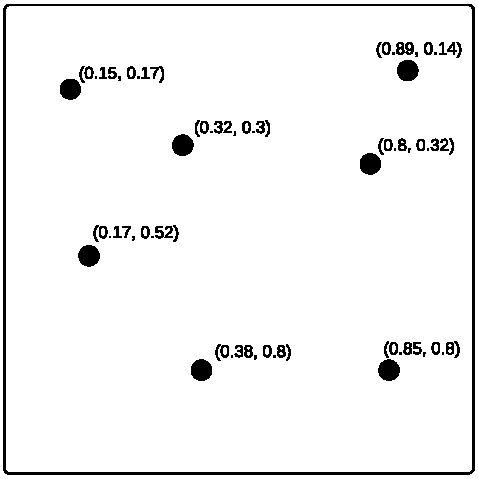
\includegraphics[scale=0.6]{figures/2D_data_space.pdf}
	\end{center}
	\vspace{-40pt}
	\caption{Data items represented as 2D points in the space $[0, 1]^d$ (not to scale)}
	\label{fig:data-space}
\end{wrapfigure}

The purpose of an index structure is to perform queries on the data. Common types of query include:
\begin{itemize}
	\item \textbf{Point Query} -- checks if a point $p$ exists in the structure \cite{rplus-tree}
	\item \textbf{Region/Range Query} -- return all points contained within a spatial region $r$ \cite{rplus-tree}, which is often a $d$-dimensional box \cite{r-tree, pk-tree, pyramid-tree}
	\item \textbf{\textit{k}-Nearest Neighbour Search} -- return the $k$ nearest points to a point $p$ \cite{pk-tree}
	\item \textbf{Approximate Nearest Neighbour Search} -- return an approximation of a $k$-nearest neighbour search \cite{knn-curse-of-dimensionality} (less accuracy, faster queries)
\end{itemize}

An index structure provides a mechanism for accessing multi-dimensional data, but it may not actually store the data itself. In a database for example, a point query comes in two parts: \textbf{searching} for a data point in the structure and \textbf{reading} the data from the data file represented by point (or index) \cite{rsr-tree}.

\section{Challenges in Multi-dimensional Search}
\label{sec:challenges}

A significant number of index structures were developed in the 1970s and 1980s, which were shown to provide good performance through empirical usage. Despite the efficiencies gained from these foundational structures, there are still numerous challenges to overcome. As such, work on developing new index structures has continued throughout the past twenty years \cite{md-structures-samet}. With the size and dimensionality of data increasing, some of these existing structures start to perform extremely poorly.

Four core challenges repeatedly discussed in the literature have been identified. Many attempts have been made to mitigate the effects of these challenges through new or modified index structures. This section will discuss these challenges, the impact they have on multi-dimensional search efficiency and \textit{why} they have these impacts.

\subsection{Curse of Dimensionality}
\label{sec:curse-of-dimensionality}

The curse of dimensionality is a term used to refer to the issues that occur when data with large numbers of dimensions is processed \cite{curse-of-dimensionality}. Spatial partitioning of high-dimensional points becomes difficult because large regions of the data space are empty. High-dimensional space is sparse because the number of data points that must be sampled to fill the space increases exponentially with $d$.

Sparsity causes many index structures to contain many empty or near-empty regions, resulting in a large amount of memory overhead (e.g. many regions in octrees with high $d$ are completely empty but exist anyway to due to uniformly sized regions). This is especially problematic when many of the dimensions might not tell you anything relevant about the data \cite{irrelevant-dimension}, causing large amounts of memory and computation to be wasted. Relating this back to multi-dimensional search specifically, Indyk and Motwani in \cite{knn-curse-of-dimensionality} discuss how efficient nearest neighbour queries with a small number of dimensions is ``well-solved", but with a high number of dimensions the problem is more challenging.

The majority of index structures discussed in the literature are hierarchical. Due to data sparseness caused by a higher number of dimensions, these structures often become very large and have many empty or near-empty nodes. Additionally, balanced splits and overlapping node regions cause most of the nodes to pass boundary intersection tests when a higher number of dimensions are used. This means the execution time of queries and dynamic operations tend to $O(n)$. In other words, the structures are no faster than a brute force sequential scan through a list, just with more memory overhead.

Weber, Schek and Blott in \cite{va-file} show how hierarchical index structures which perform data space partitioning tend to perform poorly when 10 or more dimensions is used. They even show that there is no index structure ``based on clustering or partitioning which does not degenerate to a sequential scan if the dimensionality exceeds a certain threshold" \cite{va-file}.

Therefore, for high $d$, sequential scan or methods based on linear data structures (e.g. lists) often provide better performance than methods which recursively decompose space into tree structures \cite{md-structures-samet}. This leads to the conclusion that the curse of dimensionality removes many of the benefits gained from using traditional index structures when high dimensional data is used.

\subsection{Variation in Data}

When developing an index structure, one does not know the nature of the input data in advance. Therefore, it is unwise to make too many assumptions when evaluating the efficiency of your structure with test data. Some datasets may be uniform, some may have noticeable skew and others may have a large number of clusters with complex shapes in data space. Different index structures are more efficient with different kinds of data. For example, octrees become inefficient with skewed data and $kd$-tree variants often have poor utilisation of nodes \cite{bkd-tree} (i.e. nodes store very few data points).

For some applications, where the input data's structure may be known in advance, this is not an issue, since an index structure known to perform well with that type of data can be chosen. If the nature of the data is not known in advance however, developing a generic index structure that provides efficient queries for \textit{all} kinds of data is challenging.

Wang et al. evaluated the PK-tree using uniformly distributed and clustered synthetic data, in addition to large real data sets \cite{pk-tree}. Berchtold et al. also used a combination of carefully generated synthetic data and real data sets when evaluating the performance of Pyramid Tree \cite{pyramid-tree}. Doing so allows for a comprehensive evaluation on how well a structure performs on different kinds of data.  Comprehensively evaluating an index structure's performance requires a varied collection of data, which includes:
\begin{itemize}
	\item Uniformly distributed data
	\item Non-uniform data (skewed and clustered)
	\item Large real world data sets
\end{itemize}	
Generating or finding these types of data \textit{and} ensuring an index structure performs well on most inputs have been found to be significant challenges.

\subsection{Dynamically Constructing Structures}

To maintain performance, it is common to impose invariants that maintain a balanced structure. An invariant is a condition or property of the index structure that \textit{must hold} to ensure good performance of queries. This is easier for static index structure because the structure is built once and never changes. When inserting, deleting or updating points with dynamic index structures, maintaining invariants can be non-trivial. An example of a dynamic index structure is the red-black tree, which repeatedly rotates components of the tree to fix broken invariants when a point is inserted or deleted \cite{introduction-to-algorithms}.

These invariants can result in \texttt{insert}, \texttt{update} and \texttt{delete} operations being slow. Creating index structures that provide fast queries without requiring invariants that are expensive to maintain is difficult. The balance between dynamic construction performance and query performance depends on the application. If the index structure must be updated often, then prioritising fast construction over fast queries may be appropriate.

\subsection{Memory Access and Paging}
\label{sec:paging}

Different index structures have different storage requirements. It is important to consider this when choosing/developing an index structure. Structures whose size in memory grows quickly as the amount of data increases may not be able to fit entirely in main memory, meaning some of it will have to be \textit{paged} in secondary memory (e.g. hard disk). This drastically affects performance, as it is much slower to access the hard disk than accessing main memory. This issue is amplified for high-dimensional data, as more memory is consumed per data item.

Some structures require little additional data to maintain the structure, such as splay trees and pyramid trees \cite{splay-tree, pyramid-tree}. These have \textit{low memory overhead}, meaning they scale well to large data sets. Other structures, such as PK-trees, require more data because more complex book-keeping is required to enable fast dynamic operations and queries \cite{pk-tree}. If a problem deals with massive amounts of data points, it may be worth using slower index structures with less overhead, in order to minimise the amount of memory used by the index structure. If the structure grows so large that it cannot fit in main memory, then \textit{any} index structure's performance will take a drastic hit because data has to be retrieved from secondary memory frequently.

For large datasets (terabytes in size, say), it is inevitable that some of the index structure will be stored in secondary memory. This core bottleneck has been identified and researchers have constructed index structures, called bucket methods, that store data items in ways that minimise I/O operations \cite{md-structures-samet}. Some structures have parameters that can be tweaked to find optimal paging with the target hardware or dataset, such as the PK-tree and pyramid tree \cite{pyramid-tree, pk-tree}.

To conclude, if the index structure is used with large, complex data items then some of it may have to be stored in secondary storage, especially if there are many data points. Designing an index structure to facilitate quick access to secondary memory and reduce query times has been the focus of many researchers in the field  \cite{rsr-tree, rs-tree}.

\section{Existing Index Structures}
\label{sec:structures}

Many index structures have been developed throughout the past forty years, such as quadtrees in the early 1970s \cite{quadtree} and splay quadtrees in 2012 \cite{splay-quadtree}. New structures are often based on older index structures, either by modifying an existing structure or combining two different structures in some way. Figure \ref{fig:structure-taxonomy} in Appendix \ref{chap:supp-material} shows a \textit{taxonomy} of index structures. This section describes some of the widely used index structures, their limitations (with respect to the challenges discussed in Section \ref{sec:challenges}) and why this led onto the development of new structures.

\subsection{Basic Structures}
\label{sec:basic-structures}

\textbf{Sequential scan} refers to the brute-force approach of searching a data set. You simply store the dataset in a linear data structure (e.g. a list) and iterate through each data item until the desired point is found. This means searching is an $O(n)$ operation. Using a standard array, insertion is $O(1)$ if new points are inserted at the end of the array and deletion is $O(n)$. There is little memory overhead for this approach, but search times will be very long if there are large number of points. Nevertheless, if the number of data items is small, a more complex index structure may not be needed.

\textbf{Search trees} are often used to order data items in a hierarchical fashion to make search faster \cite{introduction-to-algorithms}. The binary search tree, for one-dimensional data, is one of the first of these trees and is the basis of many index structures \cite{introduction-to-algorithms}. Each node stores a \textit{key}, which is a total orderable element. Each non-leaf node has at most two children, where the left child's key is less than its parent's and the right child's key is greater than or equal to its parent's. This property is referred to as \textit{key order} \cite{rst}. When inserting or deleting new points, the key order invariant must be maintained. Maintaining this invariant can be done in $O(n)$ time \cite{introduction-to-algorithms}, making insertion and deletion $O(n)$.

A point query is equivalent to checking if a certain key is stored in the tree. In the best case, we get running time $O(\log_2 n)$ for the query, as the height of the tree is $\log_2 n$. However, this performance is not guaranteed. Skewed or sorted data may result in taller trees, where there are many nodes with only left or only right children. This makes the binary tree \textit{unbalanced} (height greater than $\log_2 n$). If balance is not guaranteed, the running time of a point query is $O(n)$ in the worst case, which is no better than a sequential search.

\textbf{Balanced search trees} re-order the nodes to maintain balance (logarithmic height) when a node is inserted, updated or deleted, regardless of data skew. These operations cause dynamic index structure operations to become slower, but allow for faster queries. Examples of balanced search trees include red-black trees, AVL trees, splay trees and treaps \cite{introduction-to-algorithms}.

\subsection{Recursive Partitioning of Data Space}
\label{sec:recursive-partition-structures}

Index structures which decompose the data space into sub-spaces recursively are popular \cite{md-structures-samet}. The decomposed space is represented as a search tree. If $R$ is some $d$-dimensional data space, then $R_1,...,R_x$ are the decomposed sub-spaces (often disjoint) of $R$ . $R$ becomes the root node and $R_1,...,R_x$ become the children of $R$ in the tree representation. Each of those sub-spaces may then be decomposed in a similar way, increasing the depth of the tree.

This is useful because it allows large amounts of the data space to be discarded from consideration at once. Consider a point query with a point $p$. $p \in R$ since R is the entire data space. Assuming a disjoint decomposition was used, if $p \in R_1$ then $p \not\in R_2,...,R_x$. Since it is known that $p$ is only in $R_1$, only $R_1$'s children need to be checked -- the rest of the tree can be \textit{ignored}.

\subsubsection{Quadtrees}

A quadtree is one of the earliest index structures based on disjoint recursive decomposition of space, specifically created for two-dimensional space \cite{original-quadtree}. \textbf{Octrees} are a generalisation of quadtrees to $d \geq 2$ dimensions. Throughout the past forty years, many variations of the quadtree have been produced. Hanan Samet produced a survey describing many uses and variants of this data structure in  \cite{quadtree} and twenty years later, there are even more variants. Several variants are discussed in this review, but it is beyond the scope of this report to list all of them.

PR quadtrees are a commonly used quadtree which partition the data space into four uniformly sized sub-spaces. This process can be repeated recursively to produce a grid with increasingly smaller cells. Figure \ref{fig:quadtree-clustered} shows an example of a PR quadtree decomposition of some data. Notice how the underlying data space is decomposed in the same way, regardless of where the points in the dataset are in the space.

An advantage of PR quadtrees is that there is no overlap between the spatial regions represented by two sibling nodes. This greatly simplifies \texttt{insert}, \texttt{update} and \texttt{delete} operations. However, they do not perform well with \textbf{non-uniform} data. So if there are clusters or skews of data, then there will be many empty (or near empty) quadtree nodes/regions (see Figure \ref{fig:quadtree-clustered}). These unnecessary nodes in sparse regions of the data space may be searched during a query, reducing performance.

\begin{figure}
	\begin{center}
		\begin{subfloat}[PR Quadtree\label{fig:quadtree-clustered}]{%
			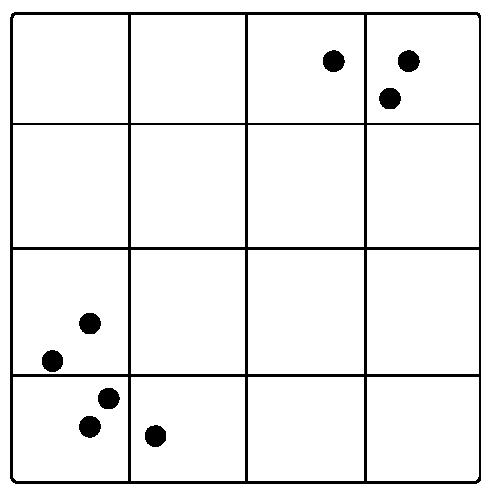
\includegraphics[scale=0.4]{figures/quadtree_clustered.pdf}
		}
		\end{subfloat}~~~~~
		\begin{subfloat}[Point $kd$-Tree\label{fig:kdtree-clustered}]{%
			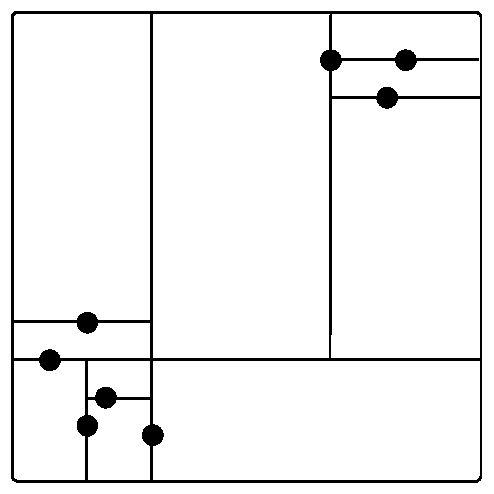
\includegraphics[scale=0.4]{figures/kdtree_clustered.pdf}
		}
		\end{subfloat}~~~~~
		\begin{subfloat}[Binary Space Partition\label{fig:bsp}]{%
			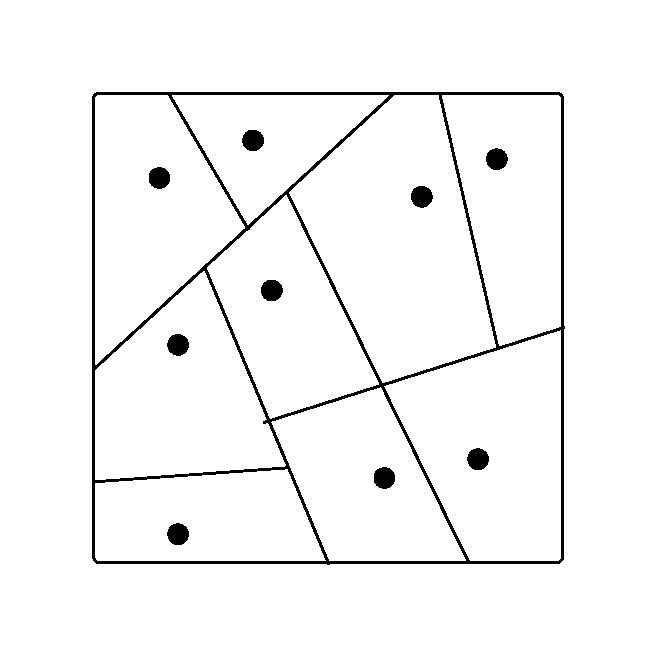
\includegraphics[scale=0.4]{figures/bsp_tree.pdf}
		}
		\end{subfloat}
	\end{center}

	\caption{Spatial Decompositions Created With Various Tree-Based Index Structures}
	\label{fig:tree-based-decomposition}
\end{figure}

\subsubsection{$kd$-trees}

$kd$-trees are similar to quadtrees in that the data space is partitioned into disjoint regions \cite{kd-tree}. Unlike quadtrees, nodes have at most two children regardless of dimensionality. Each node in the tree splits the current region of data space into two sub-regions along a single dimension $d_i$. These sub-regions are represented as two nodes, whose parent is the node representing the original region. A \textit{pivot} value $p$ is chosen for $d_i$. The left and right children contain all the data items whose $d_i$th value is less than $p$ and greater than or equal to $p$ respectively. How a $kd$-tree is built depends on how $d_i$ and $p$ are chosen, so there are many variations of this structure. There are two major types of $kd$-tree -- point and bucket (PR) \cite{md-structures-samet}. Point $kd$-trees store a single point in each node of the tree, meaning there are always $n$ nodes. Bucket $kd$-trees only store points in the leaves, which can contain multiple points.

Unlike the PR quadtree, $kd$-trees can produce non-uniform partitions, making the structure better suited to skewed or clustered data. Figures \ref{fig:quadtree-clustered} and \ref{fig:kdtree-clustered} show a PR quadtree and point $kd$-tree partition of some clustered data. Notice how there are more empty regions in the quadtree than the $kd$-tree, thus having a less efficient partition of the data.

Like binary search trees, it is ideal to maintain a \textit{balanced} tree to minimise height and ensure queries can be performed quickly. Dynamically inserting or deleting points can unbalance the tree. Variants of bucket $kd$-trees have been developed to maintain a balanced tree and fast query times. Examples of such variants include the BD-tree \cite{kdtree-v-bdtree} and KDB-tree \cite{kdb-tree}.

\subsubsection{Binary Space Partitioning}

BSP (binary space partitioning) trees are a generalisation of kd-trees that use hyperplanes (lines in 2D, planes in 3D) to recursively partition the data space \cite{bsp-tree}. That is, it partitions data space $S$ into two disjoint sub-spaces $S_1$ and $S_2$. This process is repeated recursively using different hyperplanes for each split. A BSP tree decomposition is illustrated in Figure \ref{fig:bsp}.

Optimal BSP trees allow efficient point queries to be performed by discarding as many points as possible at each level of the tree (i.e. the tree has low height). Finding optimal BSP trees for a given set of data points is an $\mathbb{NP}$-complete problem \cite{bsp-np-hard}. When inserting, updating or deleting points a new optimal partitioning must be computed to minimise tree height, making dynamic operations very slow. Therefore, BSP trees are better suited for static data because an optimal tree can be \textit{pre-computed} and loaded into main memory during program initialisation.

\subsubsection{Skip Quadtree}

Despite the original quadtree structure being developed approximately forty years ago, researchers are still enhancing the index structure's performance in new ways. A relatively new data structure, the skip quadtree, is ``simple" to implement and benefits from low memory overhead \cite{skip-quadtree}. \textbf{Skip quadtrees} were developed with range queries in mind and are based on the concept of compressed quadtrees. \textbf{Compressed quadtrees} compress paths of nodes which only have a single non-empty child into a \textit{single node} \cite{compressed-quadtree}, which combats the effects of skewed data.

Skip quadtrees combine one-dimensional skip lists \cite{skip-quadtree} and compressed quadtrees to create an index structure with $O(\log n)$ point queries and $O(\epsilon^{1 - d} \log n + k)$ \textit{approximate} range queries, where $k$ is the size of the range and $\epsilon$ is the approximation factor that controls the accuracy of the range query \cite{skip-quadtree}. However, skip quadtrees may not be efficient for very datasets because they were not constructed with paging in mind.

\subsection{Bucket Methods}
\label{sec:bucket-methods}

\textbf{Bucket methods} were developed to increase I/O efficiency for large datasets that are paged in secondary memory. Such structures were designed to minimise the number of I/O operations (secondary memory accesses) required to perform queries (see Section \ref{sec:paging}). These methods group points into contiguous memory called \textbf{buckets}, which are the same size as a page in secondary memory. To reduce the number of I/O operations required to perform a query, bucket methods aim to fill each bucket with as many nodes as possible \cite{md-structures-samet}.

There are two types of bucket methods \cite{md-structures-samet}:
\begin{itemize}
	\item \textbf{Overlapping Decomposition} -- these ensure that each bucket has a \textit{minimum} number of data items it must contain, which increases fanout and thus, search times. However, in the process of ensuring each bucket has a minimum amount of used capacity, the bounding regions of buckets in data space may begin overlapping. Overlapping regions means more nodes must be checked when performing a query, increasing search times.
	\item \textbf{Disjoint Decomposition} -- these ensure that there is \textit{no overlap} between buckets. This means less nodes need to be checked in a query, but there is no guarantee on how much each bucket is filled, potentially increasing the number of I/O operations performed
\end{itemize}

\textbf{Fanout} refers to the amount of children each node have on average. Higher fanout results in a search tree with lower height, which means less nodes are accessed on average when searching for a point. Node access is particularly expensive when the tree has been paged into secondary memory, so some bucket methods aim to increase fanout (e.g. TV-tree \cite{tv-tree} and A-tree \cite{a-tree}).

\subsubsection{B-Trees and B${}^{+}$-Trees}

The B-Tree was developed by Rudolf Bayer in 1972 and is often used for databases or file-systems \cite{ubiquitous-btree}. It is a one-dimensional search tree which allows for point queries, insertions and deletions to be performed in $O(\log n)$ time \cite{btree}. B-trees maintain key order, but allow nodes to have more than two children, making them a generalisation of binary search trees.

B${}^{+}$-trees are B-trees where only the \textit{leaves} contain the actual values of the data \cite{ubiquitous-btree}. This means all non-leaves simply contain pointers to, or the keys of, their children. B${}^{+}$-trees ensure that each bucket is at least 50\% full \cite{md-structures-samet, ubiquitous-btree}, which leads to less I/O operations. This is a very attractive property, as it can greatly speed up query times for large data sets. There have been many attempts to generalise the B-tree to a multi-dimensional setting while retaining this property. The k-d-B tree \cite{kdb-tree} and BV-tree \cite{bv-tree} are two examples of such attempts. Freeston in \cite{bv-tree} discusses how this ``apparently simple" objective has proved extremely difficult to achieve.

\subsubsection{R-Tree Family}

An R-tree can be thought of as a B${}^{+}$-tree that can handle multi-dimensional data, supporting data items that have non-zero size in data space (i.e. regions) \cite{r-tree}. This means nodes are represented using \textit{hyper-rectangles} that define the region of the data space all of the node's children are contained in. The running time for queries is $O(n)$ in the worst case, but expected performance is much higher. There are many variations of R-trees that have improved performance, such as R*-trees \cite{rstar-tree}, R+-trees \cite{rplus-tree}, SS-trees \cite{ss-tree}, RS-trees \cite{rs-tree} and Hilbert R-Trees \cite{hilbert-rtree}. Combinations of these variations also exist, such as SR-trees \cite{md-structures-samet} and RSR-trees \cite{rsr-tree}.

R-tree based structures use overlapping decomposition, which is a key performance issue \cite{pyramid-tree}. If you have a point contained in $m$ nodes' regions, all $m$ nodes could be searched. This severely limits the performance of R-tree based index structures with data spaces that have a \textbf{large} number of dimensions (see Section \ref{sec:curse-of-dimensionality} for more details).

\subsubsection{PK-Tree}

PK-trees (Pyramid K-instantiable trees) are a family of structures based on kd-trees that were created specifically to handle high-dimensional data \cite{pk-tree}. They are similar to bucket methods, but instead of imposing a minimum number of points per bucket, they impose a maximum. Imposing this maximum (called the $k$-instantiation value) results in a reduced amount of I/O operations \cite{md-structures-samet}. PK-trees bound the height of the tree to $O(\log n)$ for some data. Through tests on synthetic and real data, the PK-tree has been shown in greatly outperform the SR-tree and X-tree \cite{pk-tree}, especially for higher dimensions.

However, there are some caveats. In order for the PK-tree to have $O(\log n)$ height, certain constraints must be applied to the distribution of the data. Furthermore, the pagination of the index structure which minimises I/O operations depends on the value of $K$ (the number of children a node can have) and the size of the actual hard disk pages used by the operating system \cite{pk-tree}. The amount to split each dimension at each level is also configurable, so there are many parameters to tweak to achieve the proposed performance. Additionally, as discussed in Section \ref{sec:curse-of-dimensionality}, the PK tree's performance on very high dimensional data will be still be poor, because most index structures that decompose the underlying data space perform poorly when $d$ is high.

PK-trees are also complicated to implement. This problem is exacerbated by having to tweak many different parameters and be careful about what kind of data is stored in the tree. Therefore, due to their complexity and poor performance on very high dimensional spaces, PK-trees have not been widely adopted \cite{md-structures-samet}.

\subsection{Structures Tailored to High-Dimensional Data}
\label{sec:high-dimensional-structures}

Section \ref{sec:curse-of-dimensionality} discusses how higher dimensional data spaces cause index structures which perform well on low dimensional data to degenerate and provide poor performance. There have been efforts to develop index structures which still perform well in these data spaces. Many different approaches have been used, such as tree-based spatial decompositions, distance-based methods, dimension reduction and non-hierarchical, sequential methods. Some of the more influential data structures from the literature have been identified and are described here.

\subsubsection{X-Tree}

R-tree based index structures often struggle to provide efficient queries in high-dimensional space, because the hyper-rectangles or spheres tend to overlap more \cite{pyramid-tree}. X-trees \cite{x-tree} try to reduce overlap by extending the capacity of nodes/buckets if creating a new node would result in an overlap (these are called supernodes). X-trees outperform most R-tree variants \cite{x-tree}. However, Berchtold et al. show in  \cite{pyramid-tree} show the structure still degenerates at higher dimensions ($d \geq 10$) \cite{pyramid-tree}.

\subsubsection{Distance-Based Methods}

When there are a large number of dimensions, determining which dimensions are actually relevant for searching can be difficult. In these cases, \textbf{distance-based methods} may be useful. They use the similarity (distance in data space) between each pair of points to deduce more information about the relationships in the data and provide faster search \cite{md-structures-samet}. There are two major types: \textbf{pivot-based}, which choose a subset of all points in the dataset to base distance measurements on, and \textbf{cluster-based}, which partition the dataset's points into spatial regions called clusters that are used to compute distances \cite{md-structures-samet}. A notable distance-based index structure is the M-tree, which combines R-trees with distance-based techniques to perform high dimensional search with dynamic datasets \cite{m-tree}.

\subsubsection{Dimension Reduction}

One method of mitigating the effects of the curse of dimensionality is reducing the dimensionality of the dataset and then using an existing structure which is known to have good performance with low dimensional data. One example of this is principal component analysis (PCA) \cite{pca}, which transforms a data space into one with less dimensions, using correlations in the data to deduce with dimensions are the most useful for discrimination \cite{pca}. However, by reducing the dimensions using PCA some information is lost and the results of queries will not be exact. Note that PCA is an equivalent technique to SVD (Singular Value Decomposition) \cite{md-structures-samet}.

PCA struggles with dynamic data; if the data changes then the computed transformation will go out of sync and queries will be even less accurate. The transformation could be re-computed whenever a point is added, removed or changed but doing so takes a very long time, making dynamic operations really slow. Therefore, these dimension reducing techniques are suitable to static datasets where full accuracy is not required.

\subsubsection{Pyramid Tree}
\label{sec:pyramid-tree}

The pyramid tree is specifically targeted towards high-dimensional data \cite{pyramid-tree}. It partitions the data space into $2d$ pyramids and map $d$-dimensional data items to \textbf{one-dimensional space}, storing the mapped 1D points in a B${}^{+}$-tree. This one-dimensional representation is achieved by describing a data point in terms of \textit{which} pyramid it is contained in and \textit{where} in the specified pyramid it is. Queries are given as $d$-dimensional points which are reduced to one dimension before they're applied, reducing the effects of the curse of dimensionality. Even though data points are stored in a one-dimensional B${}^{+}$-tree, the original data is maintained since the original $d$-dimensional point is stored alongside its 1D representation. Hence, pyramid trees reduce the dimensionality of the data but retain all of the original information, unlike PCA.

B${}^{+}$-trees provide efficient \texttt{insert}, \texttt{update} and \texttt{delete} operations \cite{ubiquitous-btree}, meaning the corresponding operations are also efficient with pyramid trees. The pyramid tree's range query performance, \textit{relative} to other index structures such as X-trees, increases as $d$ does \cite{pyramid-tree}. This structure has low memory overhead because, in addition to B${}^{+}$-tree overhead, one extra value is stored per point.

Since the pyramid tree mitigates the curse of dimensionality, provides dynamic operations, uses a bucket method to store the 1D points and handles skewed data (using the Extended Pyramid Technique \cite{pyramid-tree}), the structure considers all four challenges discussed in Section \ref{sec:challenges}. Tests performed by Berchtold et al. show that the Pyramid Tree is successful at tackling these challenges \cite{pyramid-tree}.

\subsubsection{Embedding Methods}

Embedding methods are combinations of dimension reduction and distance-based methods \cite{md-structures-samet}. They use \textit{approximated} distances between points in reduced space to perform \textit{exact} queries. An example of an embedding method is FastMap \cite{fast-map}.

\subsubsection{Non-Hierarchical Methods}

Focus is turning towards sequential scan and linear data structures for faster search with high-dimensional data \cite{md-structures-samet, va-file}. This is because hierarchical index structures based on data space partitioning perform poorly on a higher number of dimensions (see Section \ref{sec:curse-of-dimensionality}). Furthermore, for large datasets that must be stored in secondary memory, sequential scan may also outperform hierarchical methods, because data items are stored contiguously and read sequentially, thus requiring less I/O operations. The VA-file is a method based on sequential scan, which is shown to consistently outperform sequential scan and the X-tree as the number of dimensions increase on real datasets \cite{va-file}.

Another non-hierarchical index structure that has been used are hash maps \cite{md-structures-samet}. One approach is to define one primary bucket in the hash map for each grid cell (region of data space), which can hold $x$ points. If a primary bucket has more than $x$ points, then an overflow bucket is constructed. This bucket is linked to the primary bucket it spawned from, similar to the chaining conflict resolution mechanism for 1D hash tables \cite{introduction-to-algorithms}. Notable hashing techniques for multi-dimensional search include MDEH (multi-dimensional extended hashing) and PLOP (piecewise linear order preserving) hashing \cite{md-structures-samet}.


\subsection{History-sensitive Structures}
\label{sec:history-sensitive-structures}

Given the same data twice, most structures will behave exactly the same. That is, how the structure builds itself and access times have little, if any, variation. There are some structures which are \textbf{history-sensitive}, meaning that their behaviour is either non-deterministic, involving some element of randomness that affects how the structure performs over time, or self-adjusting, changing itself based on how the stored data is accessed. These can allow structures to be much more dynamic and adjust themselves to perform optimal search based on the application it is being used in. Two of these structures, the quadtreap and splay quadtree, are described here.

\subsubsection{Quadtreap}

A treap is a randomised search tree used to store one-dimensional keys, which combines a binary search tree with a heap by maintaining both \textit{key-order} and \textit{heap-order} (nodes ordered by the randomly assigned probabilities) \cite{quadtreap}. The main advantage of the quadtreap is that $\log n$ height can be maintained, even when dynamically inserting and removing points, with ``high probability" \cite{quadtreap}.

A quadtreap is a combination of a compressed quadtree and a treap. Tree rotations are used to maintain a balanced height when the tree is modified. Let $h$ be the height of the tree. Running times for \texttt{insert} and point queries are $O(h)$, and \texttt{delete} is performed in $O(h^2)$. This means the \textit{expected} times for \texttt{insert} and \texttt{delete} are $O(\log n)$ and $O(\log^2 n)$ respectively.

\subsubsection{Splay Quadtree}
\label{sec:splay-quadtree}

Splay trees are one-dimensional index structures which make use of a splaying operation to achieve fast dynamic operations \cite{introduction-to-algorithms}. A splay tree is \textit{self-adjusting}, which means it is ``a data structure that reorganises itself to fit the pattern of access." \cite{splay-quadtree} This is achieved with the splaying operation, which performs a series of $O(1)$ tree rotations to maintain a balanced tree with low height.

Park and Mount, the creators of the quadtreap \cite{quadtreap}, stated ``there is no comparable self-adjusting data structure for storing multi-dimensional point sets" with regard to splay trees \cite{splay-quadtree}. Hence, they developed the splay quadtree, which combines BBD-trees (balanced box decomposition trees) with quadtrees by making use of an equivalent splaying operation on BBD-trees. Park and Mount proved good bounds on the running time of dynamic operations and queries.

The structure is complicated to implement and no papers evaluating its performance empirically have been published. Currently, the splay quadtree remains a purely theoretical structure.
\section{Evaluating and Choosing an Index Structure}
\label{sec:comparison}

\subsection{Measuring Efficiency}
\label{sec:measuring-efficiency}

One can measure the efficiency of an index structure by simply measuring the amount of time it takes perform dynamic operations and queries \cite{dynamic-data-structures}. In addition to execution time, one must also consider how much memory overhead is produced by the index structure. Such overhead may not be an issue for small data sets, but when your index structure becomes very large, it must be considered due to the issues discussed in Section \ref{sec:paging}. Measurements of index structure efficiency include:
\begin{itemize}
	\item \textbf{Structure Size} -- memory required to store the structure, relative to dataset size
	\item \textbf{Construction Time} -- how long it takes to construct a structure storing $n$ points
	\item \textbf{Dynamic Operation Execution Time} -- execution times of \texttt{insert} and \texttt{delete} operations
	\item \textbf{Query Execution Time} -- execution times of point, range or nearest neighbour queries
\end{itemize}
Big-Oh notation \cite{design-analysis-algorithms} refers to the worse case execution time of an algorithm, often with respect to the size of the input. This is used to bound the worst, average or expected execution time of an algorithm. This can be used to construct theoretical performance measurements for an index structure and if often used to guide the development and evaluation of index structures structures (e.g. in  \cite{splay-quadtree}).

The focus of bucket methods is to minimise I/O operations while still retaining well-balanced search trees. Therefore, in addition to the runtime of each operation, the number of I/O operations, or \textbf{page accesses}, is often measured (e.g. \cite{pk-tree, pyramid-tree, x-tree}). In conjunction with CPU processing time, page access count can give good insight into how efficient an index structure is for large datasets.

\subsection{Deciding on an Index Structure}
\label{sec:structure-decision}

While some structures are generally less efficient than others, such as the R-tree when compared to X-tree, the behaviour of index structures typically depends on the input data. In other words, there is no ``best" structure. Choosing the best index structure is \textit{task-dependent}. There are many factors to consider when choosing an index structure, some of which are listed below.
\begin{itemize}
	\item how many points will the structure contain?
	\item how many dimensions does the data have?
	\item how frequently will the data be modified, if at all?
	\item do queries have to be performed near real-time or is it acceptable to wait a few minutes?
	\item what distributions will the input data have? will they be uniform or highly skewed?
\end{itemize}

Note that this is by no means an exhaustive list. Table \ref{tab:comparison} in Appendix \ref{chap:supp-material} lists some of the index structures discussed in this review and their strengths and weaknesses.

The strengths and weaknesses of the structures discussed in the review will now be summarised. B${}^{+}$-trees are very popular for one-dimensional data because they are fast, simple and have low memory overhead \cite{ubiquitous-btree}. Quadtrees, kd-trees and R-tree variants have good performance on multi-dimensional data (e.g. for geometric optimisation of a 3D scene \cite{kd-tree-gpu}) and are simple to implement (no complex invariants to maintain). However, performance starts to decrease as you increase the number of dimensions. There is a need for structures which can perform efficient queries in high-dimensional space, so structures such as the pyramid tree and PK-tree were developed \cite{pk-tree, pyramid-tree}. For even higher dimensions (e.g. $d \geq 10$), it has been shown that non-hierarchical methods, such has hash-based structures or sequential scan variants, may provide better performance.
\section{Parallel Search}

When it is desired to increase the efficiency of some computational task, it is common to consider parallelisation. In the context of multi-dimensional search, this means we want to determine whether or not it's possible to perform the dynamic operations and queries of an index structure in parallel, so that we reduce runtime by solving multiple parts of the problem at once.

\textbf{Multi-core parallelisation} runs tasks in parallel on different CPU cores, which can be achieved by executing a program on multiple processes or threads on the host operating system. While it is possible to parallelise index structures on multi-core processors, prior research appears to focus on many-core (see  \cite{btree-gpu1, btree-gpu2, btree-gpu3, traversing-spatial-indexes-gpu, rtree-gpu1, rtree-gpu2}) and distributed (see \cite{fat-btree, distributed-kd-tree, distributed-md-search}) parallelisation. \textbf{Many-core} parallelisation involve a much larger number of cores than multi-core processors and thus, higher parallelisation. GPUs (graphics processing units) are examples of many-core processors, which can have thousands of cores. Despite GPUs initially being created for real-time graphics, they are increasingly being used for general-purpose computing (GPGPU) \cite{performance-tuning-gpgpu}. \textbf{Distributed computing} achieves parallelisation by having multiple physical machines performing the work, communicating with each other over a network \cite{distributed-systems}.

\textbf{Embarrassingly parallel} is a term used to describe problems which can be easily split up into independent tasks that can be parallelised \cite{designing-parallel-programs}. Queries using sequential scan can be considered embarrassingly parallel, as the linear structure can be partitioned and allocated to multiple processors which each search their own sub-structure \cite{gpu-gems-3}. Many index structures are non-linear, hierarchical structures that use some form of tree. This can make them difficult to parallelise, especially if queries require backtracking (traversing back \textit{up} the tree to take another path). This makes the parallelisation of many search structures incredibly difficult and for some, the level of communication that would be required between each parallel process is so high it dominates the time savings achieved by parallelisation, making it less efficient than a serial implementation.

A good amount of research has been performed on parallelising one-dimensional search structures, especially the B-tree, \cite{btree-gpu1, btree-gpu2, btree-gpu3, fat-btree, multidisk-btree, parallel-btree}. There has also been research into parallel multi-dimensional structures, such as the KDB-tree \cite{traversing-spatial-indexes-gpu} and R-trees \cite{master-client-rtree, parallel-rtree, rtree-gpu1, rtree-gpu2}. Recent years have seen much focus on running search on the GPU. Both the B-tree and R-tree have been successfully parallelised on the GPU and have achieved increased performance \cite{btree-gpu2, rtree-gpu1}. However, these techniques are complex and difficult to implement. It appears that parallelising multi-dimensional, even for small gains in efficiency, requires significant effort.

Furthermore, most of the multi-dimensional index structures which have currently been parallelised in the literature (e.g. R-tree) are known to degenerate when given high dimensional data (see Section \ref{sec:curse-of-dimensionality}). Since this project's focus is high-dimensional data and many of the existing parallel techniques are difficult to implement, especially for a developer with little experience with parallel or GPGPU programming, it has been decided that parallelisation will not be the focus of the project initially. For the first iteration, a serial index structure will be implemented. Depending on future research findings, later iterations may implement parallel index structures (either multi-core or many-core), but for the moment this is not the case.

\subsection{Conclusion}

In this review, the multi-dimensional search problem has been defined. Problems from many different areas of computer science, such as database querying, computer vision and visualisation, benefit from multi-dimensional search, meaning there is much benefit to gain from accelerating this process. A large array of index structures have been developed throughout the past forty years to solve this problem. Sequential scan was deemed an inefficient, na\"{i}ve solution to the problem and more sophisticated index structures were developed.

Each index structure has its own advantages and disadvantages because they were developed to tackle specific challenges. While some structures generally outperform others, there is often no ``best" structure. When considering which to use for a given application, it is important consider some key aspects about the data and the application it is being used in (see Section \ref{sec:structure-decision}). The answers to these questions can help guide the decision on which index structure to use.

The one-dimensional search problem is generally well solved and fast, dynamic index structures capable of storing huge amounts of data exist. For a low number of dimensions (e.g. 2 or 3), research has focused more on developing simple index structures with lightweight memory requirements. For high-dimensional data, focus appears to be shifting away from tree-based structures that recursively decompose space and towards linear structures. This is because tree-based approaches have been shown to have limited, if no, performance gain over sequential-based approaches when dealing with large numbers of dimensions \cite{md-structures-samet}. There has been research into parallising search, but it appears to remain a difficult problem, with little focus being given to parallelising high-dimensional search.

\chapter{Chosen Index Structures}
\label{chap:chosen-structures-hypothesis}
\vspace{-0.75cm}
\centerline{\rule{149mm}{.02in}}
\vspace{0.75cm}

This section defines the index structures implemented in this project. The reasons for choosing these structures and initial hypotheses on their performance with high dimensional data will be given.

\section{Pyramid Tree}
\label{sec:pyramid-tree-detail}

As described in Section \ref{sec:high-dimensional-structures}, the pyramid tree reduces multi-dimensional points to one dimension, which can then be used in a one-dimensional index structure. The reason this structure has been chosen is because dimension reduction techniques have been found to perform well for high-dimensional data, compared to tree-based approaches \cite{md-structures-samet}. The original Pyramid-Tree paper showed good performance on uniformly distributed data and a real dataset (with the Extended Pyramid-Technique), when compared to Sequential Scan and the competitive X-tree \cite{pyramid-tree}. There are two fundamental differences between the focus of the paper's analysis and what this project is trying to achieve:
\begin{enumerate}
	\item the paper's analysis is for \textit{range} queries, whereas this project is assessing point queries
	\item the real dataset, ``a large text database extracted from WWW-pages" \cite{pyramid-tree}, contains discrete values, whereas the real datasets considered in this project are continuous, scientific datasets
\end{enumerate}
While the database is mapped to a spatial domain when stored in an index structure, the data may have different properties or distributions than continuous, spatial-based data such as the astrophysics turbulence simulation. Therefore, it was decided that the Pyramid Tree will be implemented to explore if the structure can provide equally good performance with point queries on dynamic scientific datasets.

The reduction technique will now be explained in further detail. The Pyramid tree partitions the data space into $2d$ Pyramids where each pyramid uses a $(d - 1)$ hyperplane for its base and the centre of the data space as its tip. Figure \ref{fig:pyramid-tree-pyramids} shows how the $2d$ pyramids extend from the centre point to the data space's boundaries. Each pyramid is segmented by splitting them along $(d-1)$ hyperplanes parallel to the base of the pyramid. The one-dimensional value of a point, called the \textit{pyramid value}, defines which pyramid it is in and its height in said pyramid. The spatial partition is shown in Figure \ref{fig:pyramid-tree-buckets}, where each pyramid segment has a bucket that stores the points inside that segment.

\begin{figure}
		\begin{center}
			\begin{subfloat}[$2d$ Pyramids in 2D Data Space\label{fig:pyramid-tree-pyramids}]{%
				
\includegraphics[scale=0.7]{figures/pyramid_tree_partition.pdf}
			}
			\end{subfloat}~~~~
			\begin{subfloat}[Segmented $2d$ Pyramids, Each Associated with a Bucket\label{fig:pyramid-tree-buckets}] {%
				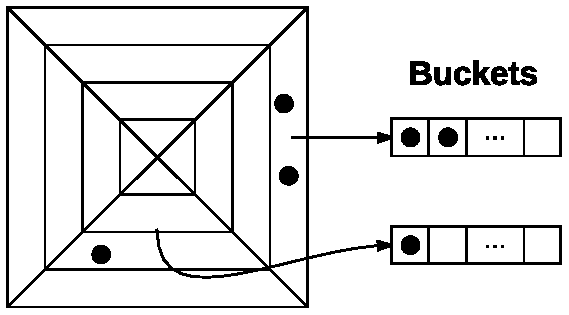
\includegraphics[scale=0.7]{figures/pyramid_tree_buckets.pdf}
			}
			\end{subfloat}
		\end{center}

		\caption{Pyramid Tree's Decomposition of Underlying Data Space}
		\label{fig:pyramid-tree-partition}
\end{figure}

More formally, the pyramid value $pv_v$ of a point $v$ is given by $pv_v = (i + h_v)$, where $i$ represents the pyramid $v$ is contained in, and $h_v$ is height of $v$ in pyramid $i$. $i$ and $h_v$ are given in Equations \ref{eq:pyramid-value-index} and \ref{eq:pyramid-value-height} respectively, where $MOD$ refers to the modulo operator.
\begin{align}
	i &= \begin{cases}
		j_{max},         & \text{if }v_{j_{max}} < 0.5\\
		j_{max} + d,   & \text{if }v_{j_{max}} \geq 0.5\\
	\end{cases}
	\label{eq:pyramid-value-index}
	\\
	j_{max} &= \left( j \;|\; \forall k \; 0 \leq j,k \leq d, j \neq k: \;\; \lvert 0.5 - v_j \rvert \geq \lvert 0.5 - v_k \rvert \right) \nonumber
\end{align}
\begin{equation}
	h_v = \lvert 0.5 - v_{i \; MOD \; d} \rvert
	\label{eq:pyramid-value-height}
\end{equation}

The following lemma shows that two distinct points can be mapped to the same pyramid value. It follows that multiple points may be stored in the same bucket. As such, bucket size will be a key performance factor for the structure and will be measured alongside execution time.

\begin{proof}[\textbf{Lemma: } For $d \geq 2$, there exist two points $x$ and $y$, such that $x \neq y$, with the same pyramid value]\mbox{}\\*
Let $d$ be the number of dimensions and $x = (x_0, x_1, \dots, x_{d -1})$, $y = (y_0, y_1, \dots, y_{d - 1})$ be two $d$-dimensional points. Without loss of generality, assume $0 \leq x_i \leq 1$ and $0 \leq y_i \leq 1$ for all $i = 1, 2, \dots, d$. Suppose $x_0 = y_0 = 0$, $x_{d - 1} = 0.1$, $y_{d - 1} = 0.2$ and $x_i = y_i = 0.1$ for all $i = 1, \dots, {d - 2}$. This means $x \neq y$. The following holds:
\begin{enumerate}
	\item $\forall k \; 0 \leq k \leq d, k \neq 0: \;\; \lvert 0.5 - x_0 \rvert \geq \lvert 0.5 - x_k \rvert$,
	\item $\forall k \; 0 \leq k \leq d, k \neq 0: \;\; \lvert 0.5 - y_0 \rvert \geq \lvert 0.5 - y_k \rvert$.
\end{enumerate}
Since $x_0 \leq 0.5$ and $y_0 \leq 0.5$, both $x$ and $y$ are mapped to pyramid 0 ($i = 0$). It follows that $h_x = h_y = \lvert 0.5 - v_{0 \; MOD \; d} \rvert = \lvert 0.5 - v_{0} \rvert = \lvert 0.5 - 0 \rvert = 0.5$. $pv_x = pv_y = 0 + 0.5 = 0.5$ and $x \neq y$, meaning two distinct points can have the same Pyramid value.

\end{proof}

\section{Pseudo-Pyramid Tree}

\begin{figure}
	\centering
	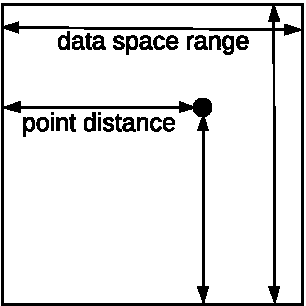
\includegraphics[scale=0.85]{figures/pseudo-pyramid_tree_point_boundary_distances.pdf}
	\caption{Computing Distance of Point Along Pseudo-Pyramid Tree Boundary for Each Dimension}
	\label{fig:point-boundary-distance}
\end{figure}

The School of Computing have an implementation of an index structure which is similar to the Pyramid Tree. Like the Pyramid Tree, it reduces $d$-dimensional points to a single dimension, which is used to search for the original point in a one-dimensional search structure. Each 1D key has its own bucket that contains references to the original points which are mapped to it. This index structure will be called the \textbf{Pseudo-Pyramid Tree}, because the reduction technique used is \textit{inspired} by the Pyramid tree, but is not the same.  To gain more insight into the performance of dimension reduction techniques in general, the Pseudo-Pyramid Tree will be implemented.

The Pseudo-Pyramid Tree reduction will now be given. To reduce a point $p$, how far along the boundary the point is in each dimension is determined (Figure \ref{fig:point-boundary-distance} gives an illustration of this). These distances are computed using Equation \ref{eq:point-boundary-distance}, where  $min_i$ and $max_i$ define the minimum and maximum bounds for dimension $i$.

\begin{equation}
	h_i(p) = \frac{p_i - min_i}{max_i - min_i}
	\label{eq:point-boundary-distance}
\end{equation}

Let $B$ be a parameter which controls how likely points will be in the same bucket and let $M = \ceil{B^{\frac{1}{d}}}$. The hashed value $h(p)$ of a point $p$ is then given by Equation \ref{eq:pseudo-pyramid-hash}. The function takes $O(d)$ time to compute because of the summation.

\begin{equation}
	h(p) = \sum_{i = 0}^{d} { \lfloor h_i(p) \times M^{i} \rfloor }
	\label{eq:pseudo-pyramid-hash}
\end{equation}

The coefficient $M$ is used to increase the magnitude of $h_i(p)$ before it is truncated with the floor function. This spaces out the mappings of points, decreasing the likelihood two distinct points will be reduced to the same value (and be stored in the same bucket). Increasing $B$ will increase $M$ because $M$ is a power of $B$. Therefore, $B$ can be used to increase or decrease discrimination between points.

\section{Bit Hash}
\label{sec:bit-hash}

% http://stackoverflow.com/questions/7403210/hashing-floating-point-values
% https://svn.boost.org/trac/boost/ticket/4038
% http://programmers.stackexchange.com/questions/63595/0x9e3779b9-golden-number
% http://stackoverflow.com/questions/4948780/magic-number-in-boosthash-combine
% http://burtleburtle.net/bob/hash/doobs.html

Bit Hash is another structure which reduces the dimensionality of points to one dimension. Instead of using a point's spatial properties, Bit Hash accumulates a hash value by hashing each individual coordinate. Each coordinate is hashed using a  32-bit floating point hashing function. The algorithms used for hashing a point and 32-bit floating point numbers is given in Algorithm \ref{alg:point-hashing} in Appendix \ref{chap:algs-and-code}.

The structure is susceptible to floating point inaccuracy because it uses the \textit{bits} of the point. On the controlled performance tests executed in this project, a point is queried using the exact same floating point values for the coordinates as when it was inserted. This means the two points have the same identical bit patterns and these errors will not occur.

Suppose the point being queried was the output of some other computation, where rounding errors may come into play. Even if the point is \textit{mathematically} identical to a point stored in the structure, rounding errors can cause the two points to have different bit patterns and thus, have different hashed values.  Despite the point being stored in the structure, it will appear as if it is not. 

This makes Bit Hash unreliable for certain applications, especially ones where the input points are the result of computations involving many arithmetic operations. Nevertheless, For the small subset of applications where all the points are pre-loaded into memory and not computed again, this can be a useful structure. Initial experiments have also shown this structure has very point query performance, so it will be explored further in this project.

\section{$kd$-tree}
\label{sec:kd-tree-detail}

The $kd$-tree is a widely used structure for both low and high dimensional data. In the literature, there is a lot of discussion as to how and why this structure performs poorly in a high-dimensional setting \cite{highd-nn, search-highd-analysis}. $kd$-trees are typically used for \textit{approximate} queries in higher-dimensional space, because they degenerate to Sequential Scan for exact range and nearest neighbour queries \cite{similarity-searching}. 

Similar to the Pyramid Tree, the focus of the literature on $kd$-trees is typically for range and nearest neighbour queries, and not point queries. Unlike the Pyramid Tree however, dynamic variants of $kd$-trees have been explored much more (e.g. in \cite{bkd-tree, kdb-tree}), with the original paper proposing operations for incremental insertion and removal \cite{kd-tree}. Assessing the suitability of multiple classes of structures provides a more comprehensive evaluation. The $kd$-tree has been chosen because it belongs to a different class of index structure than the other chosen structures, which use dimension reduction.

The structure is a multi-dimensional binary tree, meaning the number of nodes does not increase exponentially with $d$ like the octree. Instead of splitting by all dimensions at each level, $kd$-trees split the data space along a single dimension, called the \textit{cutting dimension}.

The variant of the tree implemented for this project is the point $kd$-tree (Section \ref{sec:recursive-partition-structures}). The cutting dimension at each level is chosen by cycling through the dimensions. If $n$ is a $kd$-tree node, $i$ is the cutting dimension on that node's level and $p$ is the point stored in this node, then:
\begin{enumerate}
	\item Let $q$ be any point in the left subtree rooted at $n$: $p_i > q_i$ holds
	\item Let $q$ be any point in the right subtree rooted at $n$: $p_i \leq q_i$ holds
\end{enumerate}
When inserting or querying a point $p$, the tree is traversed top-down in a similar fashion to a standard binary tree, by comparing $p_i$ to $q_i$, where $q$ is the point stored in the current node and $i$ is the cutting dimension of the current level.

The \texttt{delete} operation used is described in \cite{kdtree-remove}. Relative to \texttt{insert} and point queries, this operation requires more computation because it has to maintain the $kd$-tree invariant. To remove a point $p$, first the node containing $p$ is found using the aforementioned top-down traversal approach. Let $n$ be this node and $i$ be the current level's cutting dimension. If $n$ is a leaf, then the node can simply be deleted. Otherwise, let $n_L$ and $n_R$ be the left and right children of $n$ respectively. 

If $n_R$ exists, a node $m$ containing a point with the \textit{minimum} value for dimension $i$ is found in the sub-tree rooted at $n_R$. The points stored in nodes $n$ and $m$ are swapped and \texttt{delete($p$)} is called recursively on the sub-tree rooted at $n_R$.

If $n_R$ does not exist, node $m$ is found in the sub-tree rooted at $n_L$ instead. In this case, after \texttt{delete($p$)} has been recursively called on the sub-tree rooted at $n_L$, the $i$th value of all points stored in this sub-tree are greater than or equal to the $i$th value of the new point in $n$. Therefore, $n_L$ then becomes the \textit{right} child of $n$ to maintain the $kd$-tree invariant. 

Figure \ref{fig:kd-tree} illustrates the \texttt{insert} and \texttt{delete} operations.

\begin{figure}
	\begin{center}
		\makebox[\textwidth][c]{
		\begin{subfloat}[Inserting Point $(3, 1)$\label{fig:kdtree-insert}]{%
			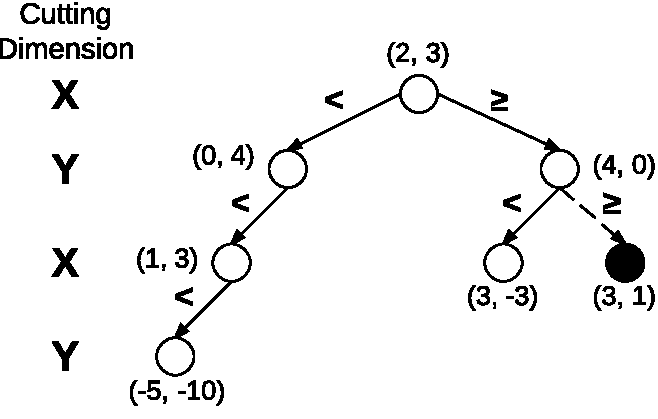
\includegraphics[scale=0.5]{figures/kdtree_insert.pdf}
		}
		\end{subfloat}~~~~
		\begin{subfloat}[Deleting Point $(0, 4)$\label{fig:kdtree-delete}]{%
			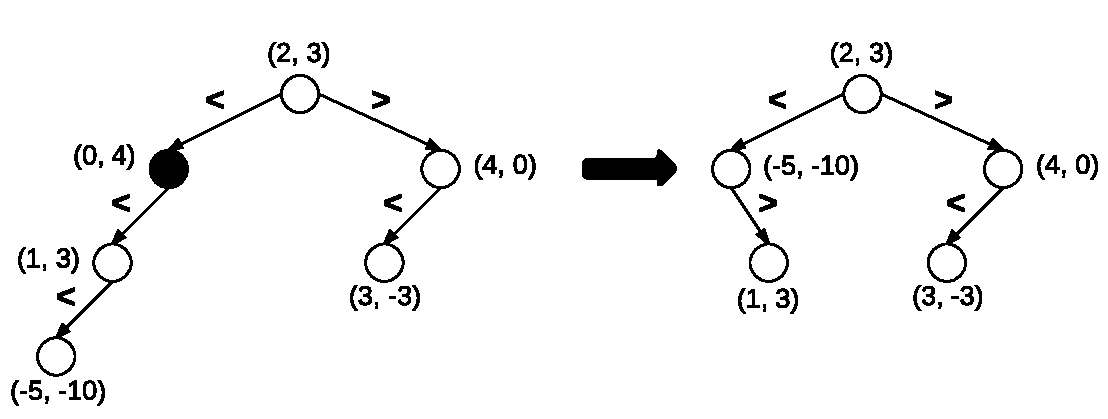
\includegraphics[scale=0.5]{figures/kdtree_delete.pdf}
		}
		\end{subfloat}	  
		}%
	\end{center}

	\caption{$kd$-tree Operations for 2D Dataset (Cutting Dimension Alternates Between X and Y)}
	\label{fig:kd-tree}
\end{figure}

\section{Main Hypothesis}
\label{sec:main-hypothesis}

Since there has been no published evaluations of the Pseudo-Pyramid Tree, no hypotheses will be made regarding the performance of the structure. It is suspected that the Pseudo-Pyramid Tree will perform well on high-dimensional data, because it is a hash-based method, but little is currently known about how well the structure's hashing function performs, so there is a little basis for such suspicion. Before starting implementation, the following hypothesis regarding the Pyramid Tree and $kd$-tree was devised:

\paragraph{\textbf{HYPOTHESIS:}} Pyramid Tree will be faster than the baselines and $kd$-trees on all evaluation datasets containing high-dimensional data ($\geq 10$ dimensions).

\paragraph{}

This hypothesis was based on the reported performance of the Pyramid Tree and $kd$-tree in a high-dimensional setting in the literature, as discussed in the previous sections. After the implementation phase, the hypothesis will be revisited to determine if it still holds, and \textit{why} it does or does not hold will be explored.
\chapter{Outline to Evaluation Approach}
\label{chap:evaluation-outline}
\centerline{\rule{149mm}{.02in}}
\vspace{2cm}

One of the project's deliverables is an evaluation of the implemented index structure(s). Multiple evaluations will be performed to guide what needs to be achieved in each iteration of development and determine how efficient the final implementations at the end of the project are. As such, evaluation forms a large part of the project. This section details what measurements will be used to evaluate implementation performance, what the baselines are (i.e. what the implementations will be compared to) and what data will be used for the evaluation.

\section{Performance Measures}

A variety of measurements have been used to evaluate the performance of index structures. Which measurements to use depend on the focus of the research and what problem the specific structure is trying to solve. Section \ref{sec:measuring-efficiency} discusses the ways index structures are commonly evaluated in the literature. This project is aimed towards accelerating index structures both algorithmically and by optimising the implementation itself. The performance analysis tools discussed in Section \ref{sec:development-tools} will be used to produce some of the chosen evaluation measures, which are:

\begin{itemize}
	\item \textbf{Total Execution Time} -- total time it took an operation to execute
	\item \textbf{Cache Hit Rate} -- rate of cache hits to misses ($\frac{\text{\# cache hits}}{\text{\# cache misses}}$)
	\item \textbf{Peak Heap Memory} -- maximum amount of heap memory used at once by the simulation 
	\item \textbf{Total Memory} -- total amount of stack and heap memory used over the entire simulation
	\item \textbf{\# Heap Allocations} -- the amount of system calls made to allocate memory on the heap
	\item \textbf{Speedup Factor} -- increase in speed when compared to another index structure (e.g. evaluation baselines). This is given by $\frac{t_1}{t_2}$, where $t_1$ and $t_2$ are the running times of the two index structures being compared.
\end{itemize}

One assumption being made about the target data is that it is dynamic, meaning points may be inserted or deleted at any time. For query performance, the evaluation will focus on the performance of point queries. Therefore, index structures will be evaluated using the performance of their \textbf{insert}, \textbf{delete} and \textbf{point query} operations.

\section{Timing Operations}
\label{sec:timing-operations}

\textbf{Amortised analysis}, introduced by Tarjan in 1985, is used to analyse the performance of algorithms over a sequence of operations, rather than an individual one \cite{amortised-analysis}. This type of analysis is typically used for algorithms where some operations take longer than others, with the goal of making operations later quicker. The amortised time complexity of an algorithm. Some index structures, particularly self-adjusting ones, have used this to bound the running time of their operations, such as the Splay Tree, Quadtreap and Splay Quadtree \cite{splay-tree, quadtreap, splay-quadtree}.

This project will use a similar concept for measuring the execution time of the structures. Instead of measuring the time of a single operartion, the times of many thousands of operations will be measured. This is to get an idea on what the runtime of an operation is on average, over a sequence of operations. This prevents single, slow operations from causing the execution time to appear worse, or short operations making the performance appear better. A typical performance test therefore has the following steps:
\begin{enumerate}
	\item \textbf{Initial Build} -- incrementally build structure by adding each point in test dataset one-by-one
	\item \textbf{Query Points} -- query each point in the dataset, which should not be in the structure
	\item \textbf{Delete Points} -- delete each point in the dataset from the structure until it is empty
\end{enumerate}
Using this process allows the runtime of large numbers of \texttt{insert}, \texttt{delete} and point query operations to be measured. Any performance tests of sequences of operations will be performed twice, and the recorded time will be the \textit{average} of the two times.

By interleaving \texttt{insert} and \texttt{delete} operations with a number of point queries, more insight can be gained into how well the implementations perform in real applications that use dynamic data structures, where the pattern of operations is less straightforward. The performance of the implementations on interleaved operations may be different from the test process described previously due to cache coherency. The contents of the cache may change frequently due to different operations being performed consecutively, potentially causing a greater number of cache misses.

The term \textbf{operation list} will be used to refer to a sequence of operations. Each operation will either be an \texttt{insert}, \texttt{delete} or point query, and will be paired with a $d$-dimensional point. These points will be pulled from the datasets described in the next section. Two main operation lists will be used for testing with a given dataset. The first, called \textbf{Insert-Query-Delete}, inserts each point in the dataset, then queries each point and finally deletes each point. The total execution time of each operation type will be measured. The second operation list, \textbf{Random Operations}, contains randomly generated interleaved operations using points taken from the target dataset and points \textit{not present} in the dataset. This is being used to measure how well the structures perform in scenarios that may occur if the structure was used in a real application, as it contains interleaved operations and queries with non-existent points.

% TODO: mention trace of Joint Contour Net behaviour that will be used to see how the index structures perform with a real application -- AND TO SEE HOW INTERLEAVED OPERATIONS

\section{Datasets}
\label{sec:datasets}

Both synthetic, artificially generated data and a real dataset will be used for the evaluation. Three types of random \textbf{synthetic} datasets will be generated, which are uniformly distributed, skewed and clustered. All generated points are in $[0,1]^d$. Multiple instances of these datasets will be used, with varying numbers of dimensions.. Using such datasets was inspired by Wang et al. and Berchtold et al., who used similar datasets to evaluate the performance of the PK-tree and pyramid tree respectively \cite{pk-tree, pyramid-tree}. The reason for testing the index structures with these datasets is that the variety of point distributions and number of dimensions should tease out which data the implementations struggle with and which they work well at.

The synthetic data was generating randomly using the \texttt{boost::random} library and the Mersenne twister pseudorandom number generator (PRNG) \cite{mersenne-twister}.  The Mersenne twister passes ``stringent statistical tests" of randomness, including diehard \cite{mersenne-twister}. \texttt{boost::random} was chosen over using the C standard library function \texttt{rand()} because the latter is platform-dependant, so it is know as to what underlying PRNG will be used and if it passes these stastical tests.

Figure \ref{fig:synthetic-data} shows 2D randomly generated points using uniform, skewed and clustered distributions. Skewed data was generated by applying a power to the number. Let $p$ be a generated point. Since $0 \leq p_i \leq 1$ for all $i \in \lbrace 1, ..., d \rbrace$, this means $p_i^e \leq p_i$ for all $e \geq 1$. This makes smaller values more likely, generating a skewed distribution of points. $e = 1.5$ was used for all skewed datasets generated. The clustered datasets contain two clusters of points, each contained within the hypercubes $[0,0.5]^d$ and $[0.7,0.8]^d$.

\begin{figure}
		\begin{center}
			\begin{subfloat}[Uniform Distribution\label{fig:uniform-distribution}]{%
				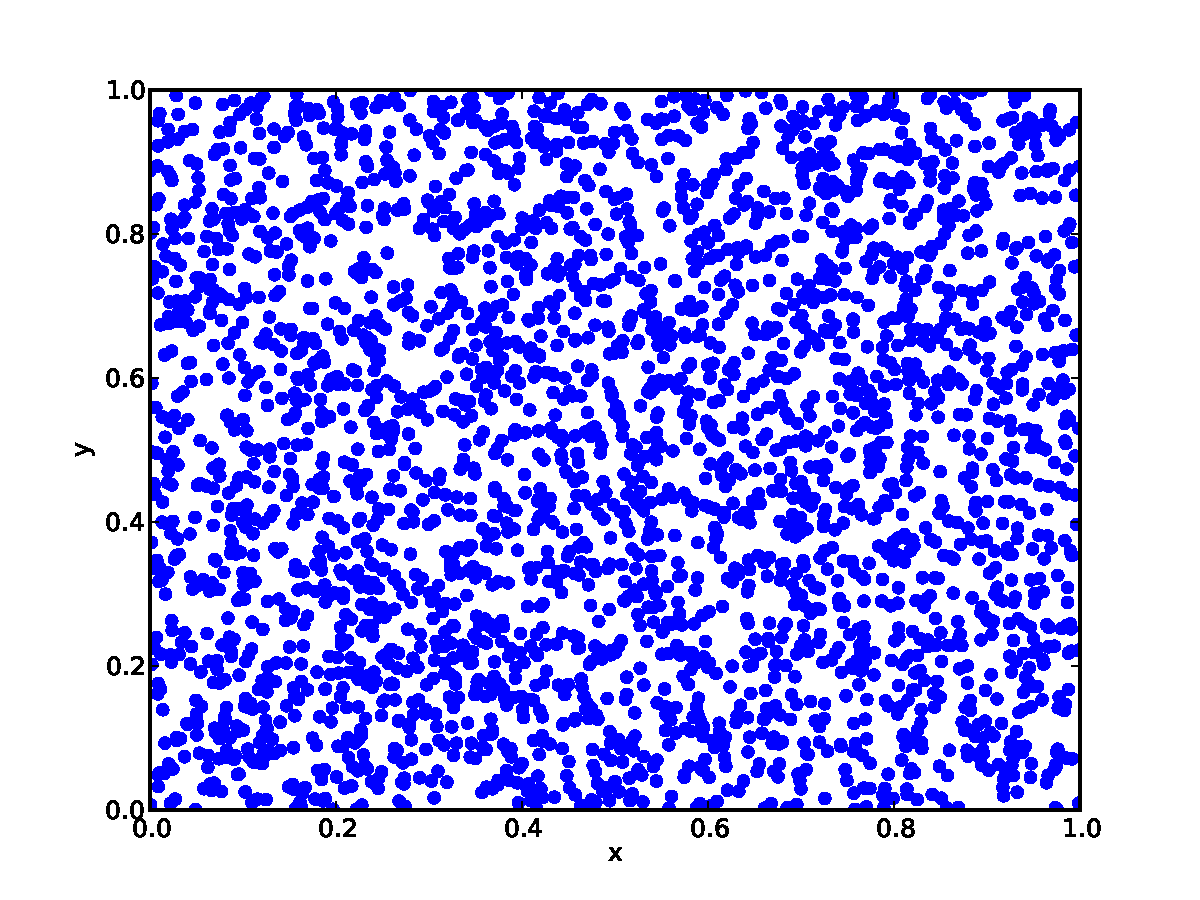
\includegraphics[scale=0.25]{figures/uniform_distribution.pdf}
			}
			\end{subfloat}~
			\begin{subfloat}[Skewed Distribution\label{fig:skewed-distribution}]{%
				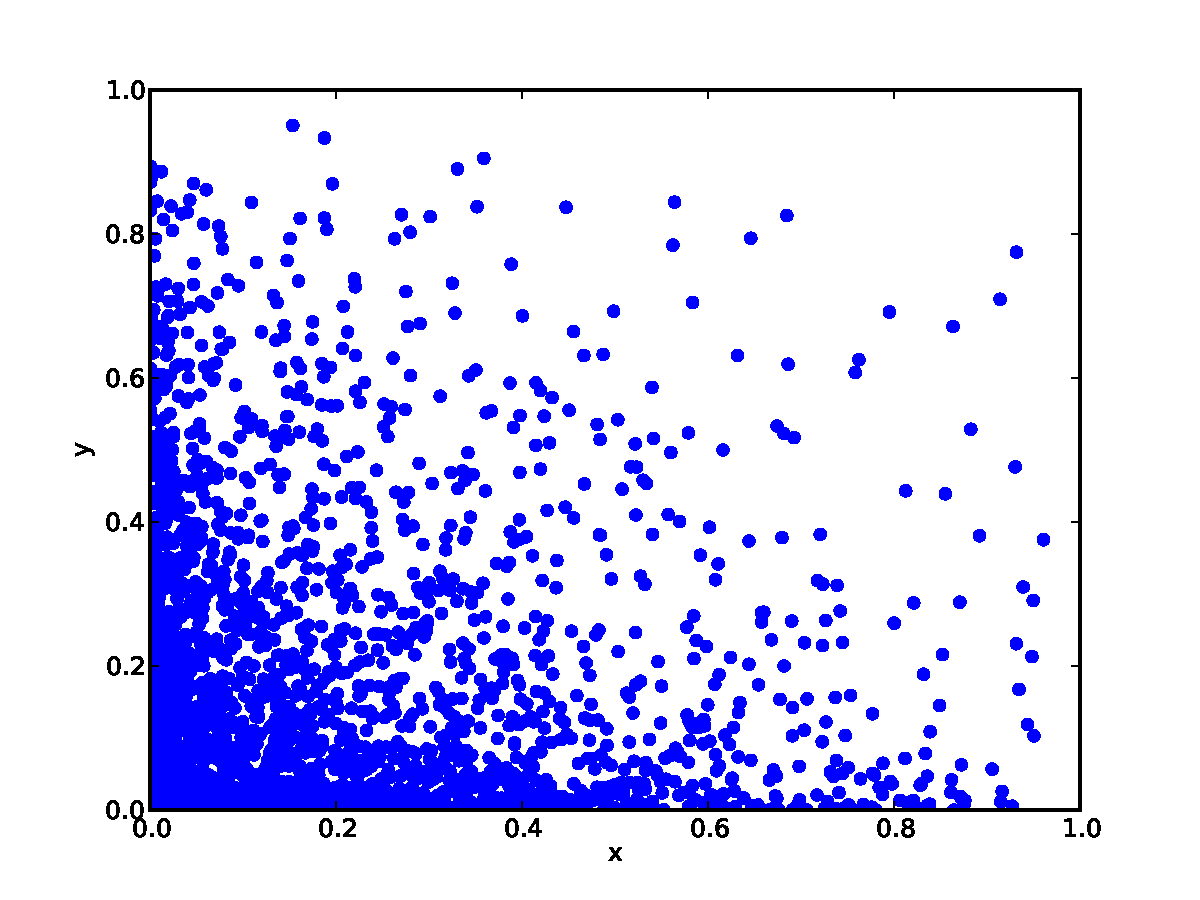
\includegraphics[scale=0.25]{figures/skewed_distribution.pdf}
			}
			\end{subfloat}~
			\begin{subfloat}[Clustered Distribution\label{fig:clustered-distribution}] {%
				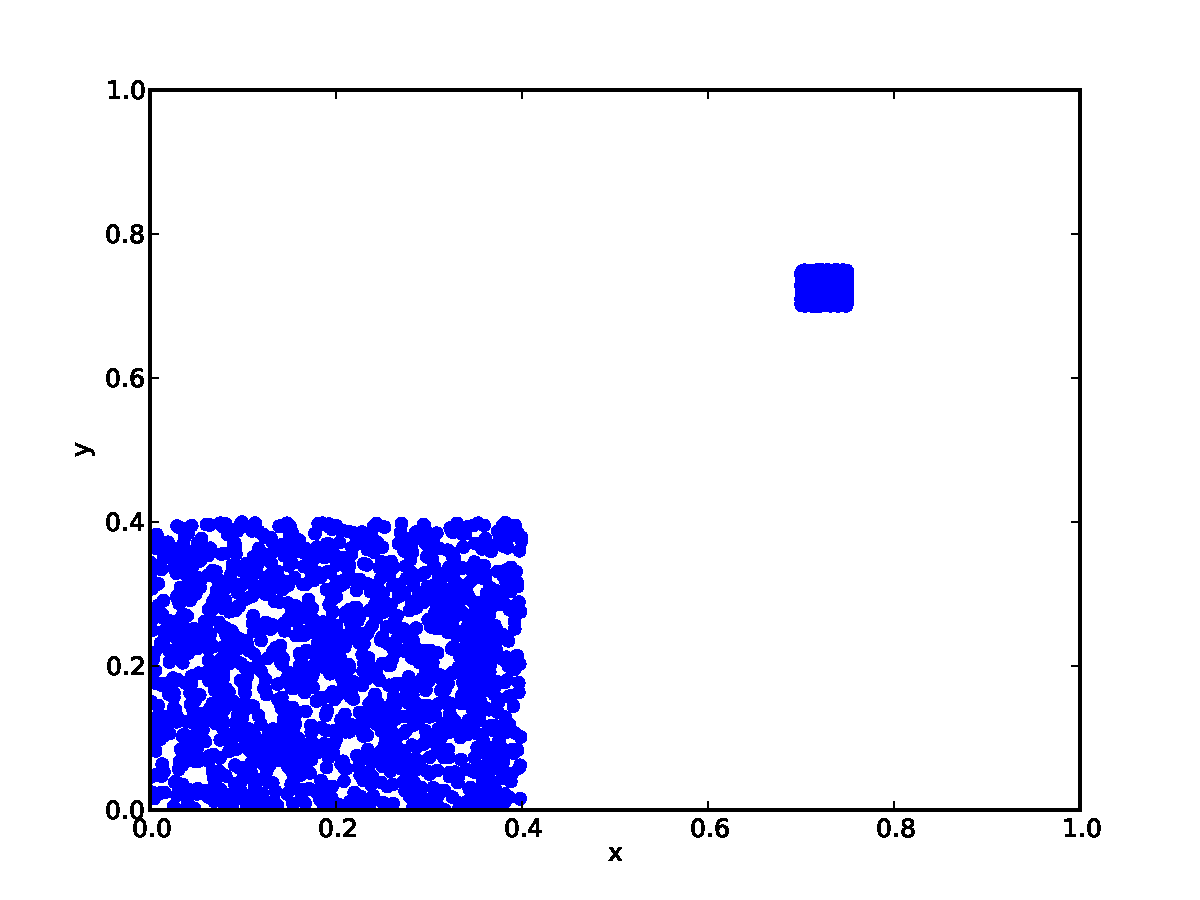
\includegraphics[scale=0.25]{figures/clustered_distribution.pdf}
			}
			\end{subfloat}			  
		\end{center}

		\caption{Three Types of Synthetic Dataset Used For Evaluation}
		\label{fig:synthetic-data}
\end{figure}

The real dataset being used for the evaluation is the result of an \textbf{astrophysics turbulence simulation}, where a $600 \times 248 \times 248$ regular mesh was used to simulate ``three-dimensional radiation hydrodynamical calculations of ionization front instabilities" \cite{astrophysics-dataset}. Figure \ref{fig:ionisation-front-instabilities} shows an example of a visualisation generated using a 2D slice of the data. Each point of the mesh has ten scalar fields, which include particle density, temperature and eight chemical species. 200 timesteps were recorded, each being approximately 126 to 128 years apart \cite{astrophysics-dataset}. For each evaluation, only \textbf{one timestep} of the simulation will be used at a time. Since some of the timesteps have different distributions, multiple tests with different timesteps may be performed.

\begin{wrapfigure}[12]{r}{0.4\textwidth}
	\vspace{-20pt}
	\begin{center}
		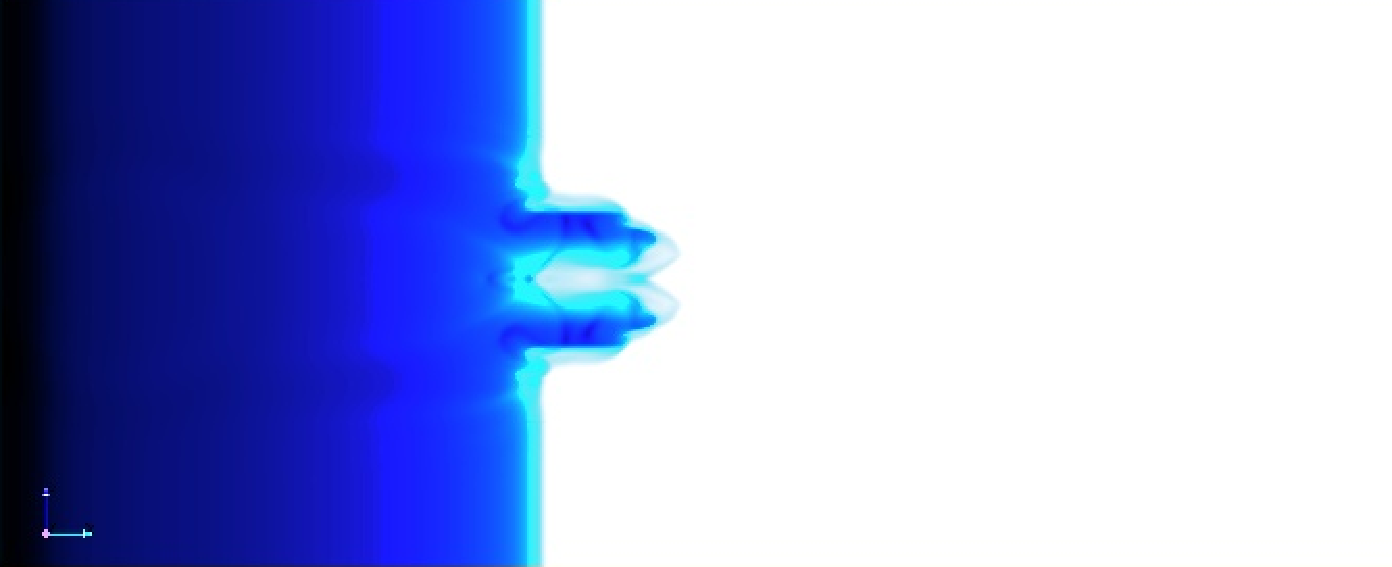
\includegraphics[scale=0.2]{figures/ionisation_front_instabilities.pdf}
	\end{center}
	\vspace{-20pt}
	\caption{Shadow Instability Forming in One 2D Slice Through the Astrophysics Dataset Over Time \cite{astrophysics-dataset}}
	\label{fig:ionisation-front-instabilities}
\end{wrapfigure}

The astrophysics was chosen because it is large (almost 37 million points) and has a high number of dimensions (10). The core focus of the project is high-dimensional data, so this data will provide a true test of how well the implementations perform with real instances of such data. The original dataset has a large number of points. For intermediate evaluations, it was decided to use smaller instances of this dataset for performance tests. Sampling a sub-region of the grid or uniformly sampling to create a dataset with a smaller resolution may introduce \textit{bias} in the data, which affects the evaluation. Therefore, smaller instances of the dataset are generated by randomly picking $n$ points from the original dataset, discarding and picking other points whenever a point that has already been sampled was chosen. By the law of large numbers\footnote{\url{http://en.wikipedia.org/wiki/Law_of_large_numbers}}, as $n$ is increased, the smaller dataset tends to being more representative of whole dataset, making this method statistically fairer.

% TODO: why choose 16?
% TODO: why 100??
% TODO: mentino skew in average runtime and say why it's a problem?
Multiple synthetic datasets with 10,000 points have been generated for each distribution, with varying numbers of dimensions. Tests using these datasets will measure the \textit{total} runtime of the operations, as the number of operations is fixed, meaning a fair comparison can be made. The structures will also be measured against data of varying size. 500,000 randomly generated points with a uniform probability distribution has been generated, which will be sampled to construct each dataset. The large dataset has 16 dimensions, which was chosen to match the tests performed by Berchtold et. al for their Pyramid Tree in \cite{pyramid-tree}. Since the number of operations is dependant on the number of points in the dataset, which varies, the \textit{average} runtime of an operation will be measured. This allows a more fair comparison between operation times of each structure to be made as the dataset size increases. The Insert-Query-Delete operation list will be used for all of these datasets. 

Timestep 100 of the astrophysics turbulence simulation will be used with a varying number of points, with both the Insert-Query-Delete and Random Operations lists. Again, the average runtime of operations will be measured Table \ref{tab:operation-lists} shows the operation lists that will be used for evaluation, which datasets the points will be pulled from, the different values the varying parameter (dimension or dataset size) will have and what performance measure will be used for an operation.

\begin{table}
	\centering
	\makebox[\textwidth][c]{%
	\begin{tabular}{|p{3.5cm}|p{3cm}|p{3.5cm}|p{4cm}|p{4cm}|}
		\hline
		\textbf{Operation List} & \textbf{Distribution(s)} & \textbf{Varying Parameter} & \textbf{Parameter Values} & \textbf{Performance Measure} \\
		\hline
		Insert-Query-Delete & Uniform, Skewed, Clustered & Dimension & 1, 2, 3, 5, 8, 10, 30, 50, 100, 200 & Total Runtime \\
		Insert-Query-Delete & Uniform & Input Size & 10, 100, 1,000, 5,000, 10,000, 50,000, 100,000, 500,000 & \parbox[t]{3in}{Average Operation\par Runtime \strut} \\
		Insert-Query-Delete & \parbox[t]{3in}{Astrophysics\par($t = 100$)\strut} & Input Size & 10, 100, 1,000, 5,000, 10,000, 50,000, 100,000, 500,000 & \parbox[t]{3in}{Average Operation\par Runtime \strut} \\
		Random Operations & \parbox[t]{3in}{Astrophysics\par($t = 100$)\strut} & Input Size & 10,000, 100,000, 500,000 & \parbox[t]{3in}{Average Operation\par Runtime \strut} \\
		\hline
	\end{tabular}}%
	\caption{Operation Lists Used for Main Evaluation}
	\label{tab:operation-lists}
\end{table}

\section{Baselines}

There is little use in measuring the performance of the implemented index structures for the purposes of evaluation if there is nothing to compare the results to. As such, two baseline index structure implementations will be developed -- \textbf{sequential scan} and the \textbf{PR octree} (see Section \ref{sec:recursive-partition-structures}). The reason for choosing sequential scan as a baseline is that it's the na\"{i}ve brute-force approach to performing search. The PR octree is the basis of many index structures, both old and new. Thus, the structure is well-known in the field and makes a suitable baseline.

These baselines have been developed in C++ to match the technology used to develop the initially implemented index structure.

\section{Environment}

The machines in the University of Leeds' School of Computing laboratory have been used to develop the index structures and measure their performance. Table \ref{tab:system-specifications} lists the hardware, operating system and tool versions these machines use.

\begin{table}[H]
	\centering
	\begin{tabular}{|r|l|}
		\hline
		\textbf{CPU} & Intel(R) Xeon(R) CPU E3-1225 V2 @ 3.20 GHz (four cores) \\
		\hline
		\textbf{Main Memory (RAM)} & 15.5 GB \\
		\hline
		\textbf{Operating System} & Linux CentOS 6.5 (Final) \\
		\hline
		\textbf{Linux Kernel Version} & 2.6.32-431.3.1.el6.x86\_64 \\
		\hline
		\textbf{C++ Compiler} & GCC 4.4.7 (Released 13/03/2013) \\
		\hline
		\textbf{Boost Library Version} & 1.41.0 \\
		\hline
	\end{tabular}
	\caption{Hardware, Operaring System and Tool Versions used for Development and Performance Testing}
	\label{tab:system-specifications}
\end{table}

\subsection{Measuring Execution Time of Code}

There are various ways of measuring the execution time of an application. Individual index structure operations are typically much lower than a second, sometimes even less than a millisecond. A high level of precision and accuracy is required because even millisecond savings are important when optimising index structure operations are required.

C/C++ come with two standard timing mechanisms. \texttt{time()}\footnote{Online documentation for \texttt{time()}: \url{http://www.cplusplus.com/reference/ctime/time/}} returns the number of seconds since the Unix epoch (00:00, 01/01/1970 UTC). Since it returns seconds, it is not precise enough for this project. \texttt{clock()}\footnote{Online documentation for \texttt{clock()}: \url{http://www.cplusplus.com/reference/ctime/clock/}}  measures the number of CPU ticks since some epoch (typically the launch of the application). The amount of real time (i.e. milliseconds, seconds, etc.) a CPU tick takes is constant, but depends on the hardware.

\texttt{clock\_gettime()}\footnote{Online documentation for \texttt{clock\_gettime()}: \url{http://linux.die.net/man/3/clock_gettime}} returns a time with nanosecond precision, but is only available on specific systems (e.g. Linux). Since the operating system used for the evaluation framework is Linux and this level of precision is desired, \texttt{clock\_gettime()} has been used for timing all operations.
\chapter{Design and Implementation}
\label{chap:design-and-implementation}
\centerline{\rule{149mm}{.02in}}
\vspace{2cm}

\section{Iteration \#1 -- Pseudo-Pyramid Tree}

This iteration deals with the low-level implementation details of the Pseudo-Pyramid Tree index structure. Different optimisation techniques are applied to the structure and multiple implementations of the Pseudo-Pyramid Tree are analysed to determine which is the fastest.

\subsection{Initial Pseudo-Pyramid Tree Implementations}

The Pseudo-Pyramid tree's reduction from $d$ dimensions to one can be seen as a hashing function, where the one-dimensional value acts as the hash to use when searching a hash table. The Initial implementation of the structure stores all the points in a single array, which hashes each point to an integer representation that acts as the key to a bucket stored in a hash map (specifically \texttt{boost::unordered\_map}, part of the Boost\footnote{\url{http://www.boost.org/}} library). A bucket is an array that contains indices to points in the single point array. Another array is used to store the sums of all stored points. This is used to speed up point queries, by comparing the sums (one comparison) of the input point to the points in a bucket. A full point comparison ($d$ comparisons) only needs to be performed if the sums match up.

No \texttt{delete} operation was provided in the original implementation of the Pseudo-Pyramid Tree, so a \texttt{delete} procedure had to be added. To delete a point $p$, the point is first hashed and the bucket containing the point is found. The index pointing to $p$ in the bucket is removed from the bucket, but the actual point itself is not removed the point array. In other words, the memory is never released until the whole structure is deleted. This makes the structure useful for batch computation because it can be discarded straight after a task, releasing all allocated memory then. However, if the structure is used as part of a long-running process then this is not suitable because there is the potential to run out of memory. This implementation shall be referred to as the \textbf{Batch Pseudo-Pyramid Tree}.

Two variants of this structure were implemented to provide a \texttt{delete} operation which releases memory. The first is the \textbf{Defragmented Pseudo-Pyramid Tree}. When a point's index is deleted from a bucket, the element at the index is marked for deletion from the array at a later time. If the number of marked elements exceeds a certain number $R$, then the $R + 1$ marked elements are erased from the vector (i.e. memory is released). The indices in each bucket are then updated to point to the correct element in the modified array. This defragmentation procedure causes \texttt{delete} operation's complexity to become $O(n^2)$.

The \textbf{Rebuild Pseudo-Pyramid Tree} uses a different strategy for releasing memory for unused points. Instead of defragmenting the array by performing a sequence of array deletions when $R + 1$ elements are marked for deletion, the entire structure is rebuilt. This new cleanup procedure starts by clearing the structure and incrementally building the new structure by only adding points \textit{not} marked for deletion. $n - R$ points will be re-inserted and insertion in the worst case is $O(n)$, meaning the worst case complexity of \texttt{delete} is $O((n - R)n)$. The larger $R$ is, the less time it takes to perform this procedure but a larger amount of allocated memory goes unused at a time.

TODO: say not using defragmented!!

\subsection{Accelerating Hash Function}

The existing Pseudo-Pyramid tree hash function is an $O(d^2)$ operation because of the inner loop that computes $\prod_{j=0}^{i}{\lbrack m_j \rbrack}$. If $m$ is changed during the structure's lifetime, the structure must be rebuilt. Otherwise the one-dimensional value of a point could change and stored points can become inaccessible. Therefore, $m$ is constant in the Pseudo-Pyramid Tree. This allows the hash function to be executed in $O(d)$ time by \textit{pre-computing} $\prod_{j=0}^{i}{\lbrack m_j \rbrack}$. This pre-computation happens when the Pseudo-Pyramid Tree is initialised. The new hash function is given in Equation \ref{eq:new-pseudo-pyramid-hash}.

\begin{multline}\\
	h(p) = \sum_{i = 0}^{d} { \lbrack \texttt{toInt}( h_i(p) \times m_i ) \times M_i \rbrack } \\
	\text{where } M_i = \prod_{j=0}^{i}{\lbrack m_j \rbrack} \;\;\; \text{for} \; 0 \leq i \leq d \\
	\label{eq:new-pseudo-pyramid-hash}
\end{multline}

Table \ref{tab:new-pseudo-pyramid-hash} shows operation execution time of the Batch Pyramid Tree using the original $O(d^2)$ hashing function and the new $O(d)$ function on a 200D dataset. Figure \ref{fig:new-pseudo-pyramid-hash} plots the performance of the Pseudo-Pyramid Tree with both hash functions alongside Sequential Scan, showing execution time against dimensionality. From the plot, it is clear that the new hashing function is superior. The old hash function caused the Pseudo-Pyramid Tree to be slower than Sequential Scan when the dimensionality exceeded a certain number ($\approx 57$). The new hash function makes the structure significantly faster than Sequential Scan, even for dimensions as high as 200.

\begin{table}
	\centering
	\begin{tabular}{|l|l|l|}
		\hline
		\textbf{Operation} & \textbf{$O(d^2)$ Function} & \textbf{$O(d)$ Function} \\
		\hline
		Insert & 1.46412 & 0.0112199 \\
		Delete & 0.730777 & 0.00625336 \\
		Point Query & 0.731469 & 0.0076015 \\
		\hline
	\end{tabular}
	\caption{Total Execution Time (in seconds) of Batch Pseudo-Pyramid Tree Using $O(d^2)$ and $O(d)$ Hash Function (200D Randomly Uniform Dataset, 10,000 operations each)}
	\label{tab:new-pseudo-pyramid-hash}
\end{table}

\begin{figure}
	\centering
	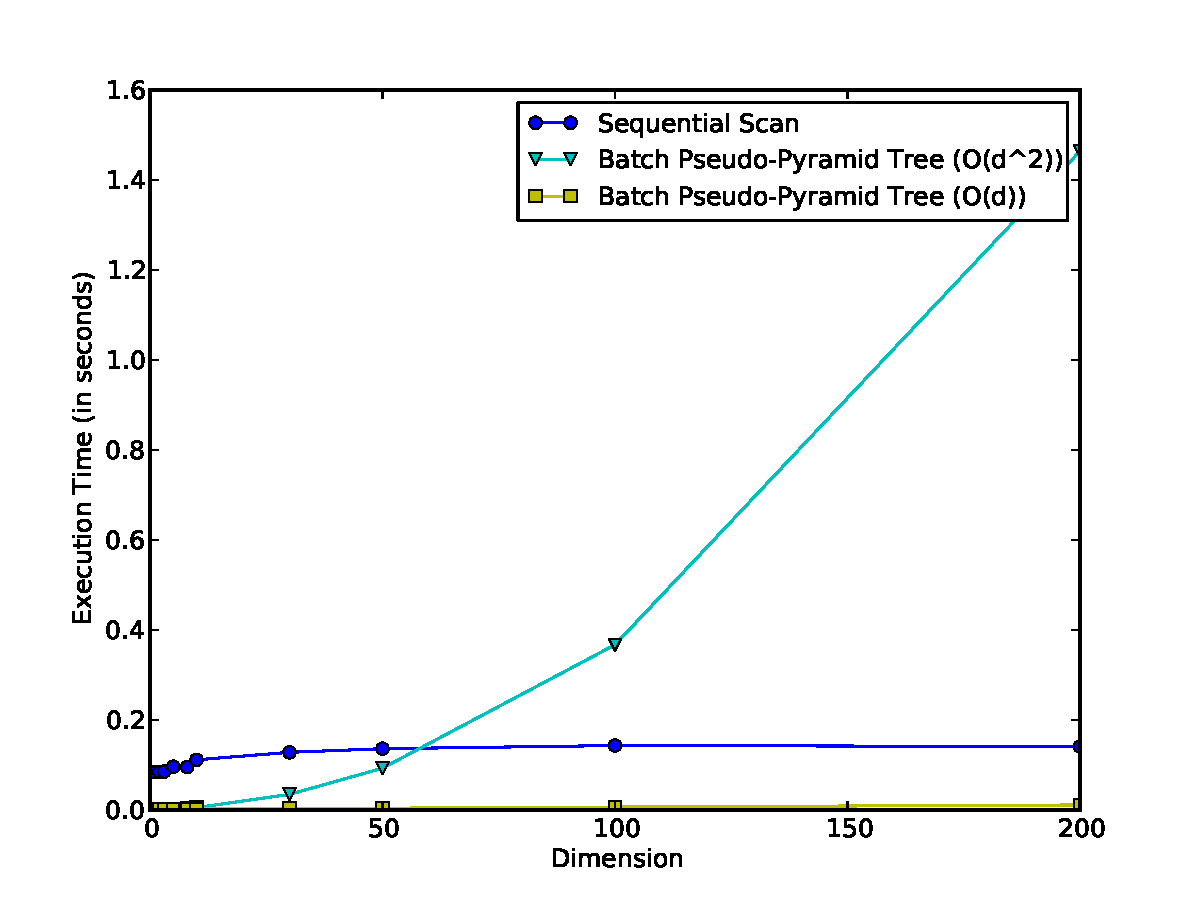
\includegraphics[scale=0.5]{figures/performance_analysis/iteration_1/new_pseudo-pyramid_hash_performance.pdf}
	\caption{\texttt{insert} Performance on Random Uniformly Distributed Datasets of Varying Dimensions}
	\label{fig:new-pseudo-pyramid-hash}
\end{figure}

\subsection{SSE Optimisation}

Since optimising the hashing function resulted in a massive speed increase, it was decided that the function would be parallelised using SSE. Considering point equality is used throughout all the index structures and will be executed many times if there are large buckets in the Pseudo-Pyramid Tree, it is worth optimising to see if there is any major speed-up. Point equality, like the hashing function, is an $O(d)$ operation. In both operations, there is loop which iterates once for each dimension, where each iteration is independent of the others. If 32-bit floating point numbers are used, then four dimensions can be processed at once using 128 bit SSE registers. Since each operation does not spend their entire time hashing or comparing points, it is not expected that a speedup of four can be achieved.

Table \ref{tab:pseudo-pyramid-sse} shows the execution times of the Pseudo-Pyramid Tree with and without SSE optimisation for the hash function and point equality. Across all three operations, the speedup averages to approximately $1.97$ when there are 200 dimensions. Note that if the number of dimensions is less than four, there is little benefit using the 128-bit SSE registers, so the structure uses the sequential hashing function and point equality check.

\begin{table}
	\centering
	\begin{tabular}{|l|l|l|}
		\hline
		\textbf{Operation} & \textbf{Without SSE} & \textbf{With SSE} \\
		\hline
		Insert & 0.0112199 & 0.00674333 \\
		Delete & 0.00625336 & 0.00313489 \\
		Point Query & 0.0076015 & 0.00298432 \\
		\hline
	\end{tabular}
	\caption{Total Execution Time (in seconds) of Batch Pseudo-Pyramid Tree With and Without SSE Optimisation (200D Randomly Uniform Dataset, 10,000 operations each)}
	\label{tab:pseudo-pyramid-sse}
\end{table}

\subsection{Bucket Pseudo-Pyramid Tree}

The index-based variants require the CPU has to fetch two elements from main memory for each point in a bucket -- the index of a point and the point itself. This also results in more random accesses in the single point array, potentially causing more cache misses, because a bucket's indices may point to distant parts of the large point array. Furthermore, having a large point array makes \texttt{delete} operations difficult to perform cheaply.

The Bucket Pseudo-Pyramid Tree implementation does not use a single array to store the points. Instead of buckets containing an array of point indices, it has an array of actual points. The goal of this variant is to increase \textbf{cache coherency} when searching a bucket, since the point array can be searched sequentially and only one memory read is required. No cleanup procedure is necessary because the memory for a point is released immediately after it's removed, by simply erasing it from the corresponding bucket's array (which is much smaller than an array containing \textit{all} the points). However, \texttt{delete} is still an $O(n)$ operation since the worst case is when a single bucket stores all $n$ points.

The order the points are stored in a bucket do not matter, the C++ \textit{erase-remove} idiom has been used to delete elements from the bucket arrays. This idiom swaps the element to delete with the last element in the array, removing the desired element when it's at the end of the array. This means there is no need to move any elements in the array to fill the gap created by removing an element, since the element removed is always at the end of the array.

\subsection{Splay Pseudo-Pyramid Tree}

Unlike the other implementations, the Splay Pseudo-Pyramid Tree does not use a hash map as the underlying one-dimensional index structure, but a splay tree. The splay tree is a self-adjusting variant of the binary search tree that uses a \textit{splaying} operation (a heuristic) to allow faster access to recently accessed elements. \cite{splay-tree}. The splaying operation achieves this by performing a series of tree rotations that move a given node up to the root of the tree. Through amortised analysis and empirical experiments, it has been shown splay trees can be more efficient than standard binary trees for a series of non-random operations \cite{splay-tree}, despite the asymptotic worst case bound being worse than binary search trees.

Nodes in the Splay Pseudo-Pyramid Tree correspond to individual buckets in the Bucket Pseudo-Pyramid Tree, meaning each node can store multiple points. Since the splay tree is implemented as a collection of heap-allocated nodes with pointers to link them, deletions are cheap as a low amount of memory needs to be de-allocated per \texttt{delete} operation. The aim is that this, combined with the self-adjusting nature of the splay tree, will produce a Pseudo-Pyramid Tree implementation that is more efficient for non-random operations used in real applications.

\subsection{Performance Timings}

All variants of the Pseudo-Pyramid Tree hash $d$-dimensional points to a one-dimensional value, which is used as a key to search for a given point in a one-dimensional structure. What varies is how points are deleted and which underlying one-dimensional structure is used. The Batch Pseudo-Pyramid Tree never releases memory after points are removed. For dynamic data which changes frequently, this may cause the machine to run out of memory, so this variant will not be explored any further.

The remaining variants of the Pseudo-Pyramid and the two baselines, Sequential Scan and Octree, were timed with the full collection of synthetic and real datasets. $B = 300000$ and $R=3000$ was used as parameters for the Pseudo-Pyramid Trees. This means the Defragmented and Rebuild Pseudo-Pyramid Tree defragment and rebuild respectively when 3001 elements have been marked for deletion.

Table \ref{tab:perf1-dimensionality} contains the \textit{total} runtime of \texttt{insert}, \texttt{delete} and point query for uniformly randomly generated points for the analysed structures. When ``-" is shown instead of the number of seconds, it means that the performance test could not finish due to the machine running out of memory. Plots with dimension against execution time are shown for \texttt{insert} and \texttt{remove} in Figure \ref{fig:perf1-dimensionality}. The execution times for skewed and clustered data was almost identical to the uniformly random datasets; for the sake of brevity, the tables and plots for these datasets have been placed in Appendix \ref{chap:supp-material}.

\begin{figure}
	\makebox[\textwidth][c]{%
		\begin{subfloat}[\texttt{insert}\label{fig:perf1-dimensionality-insert}]{%
			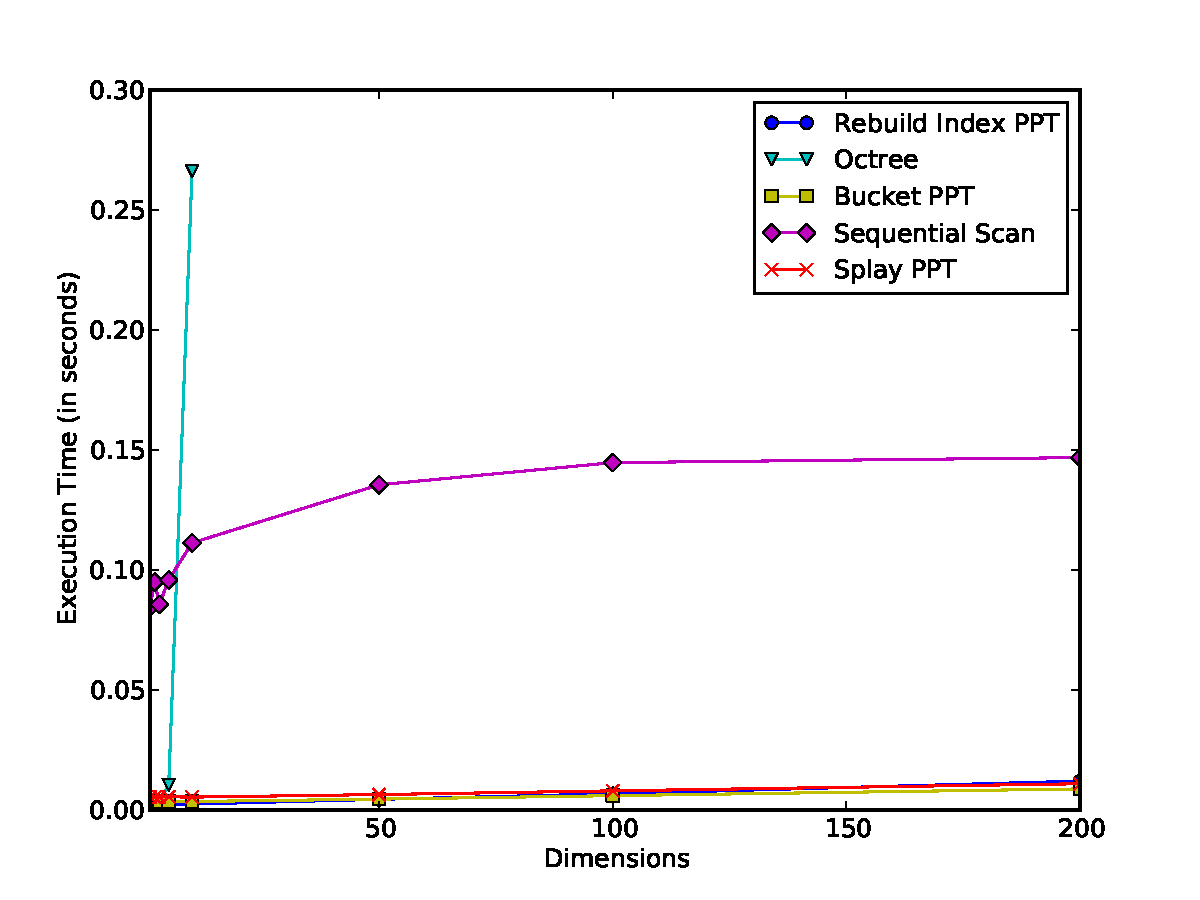
\includegraphics[scale=0.5]{figures/performance_analysis/iteration_1/randuniform_insert.pdf}
		}
		\end{subfloat}
		\begin{subfloat}[\texttt{delete}\label{fig:perf1-dimensionality-remove}]{%
			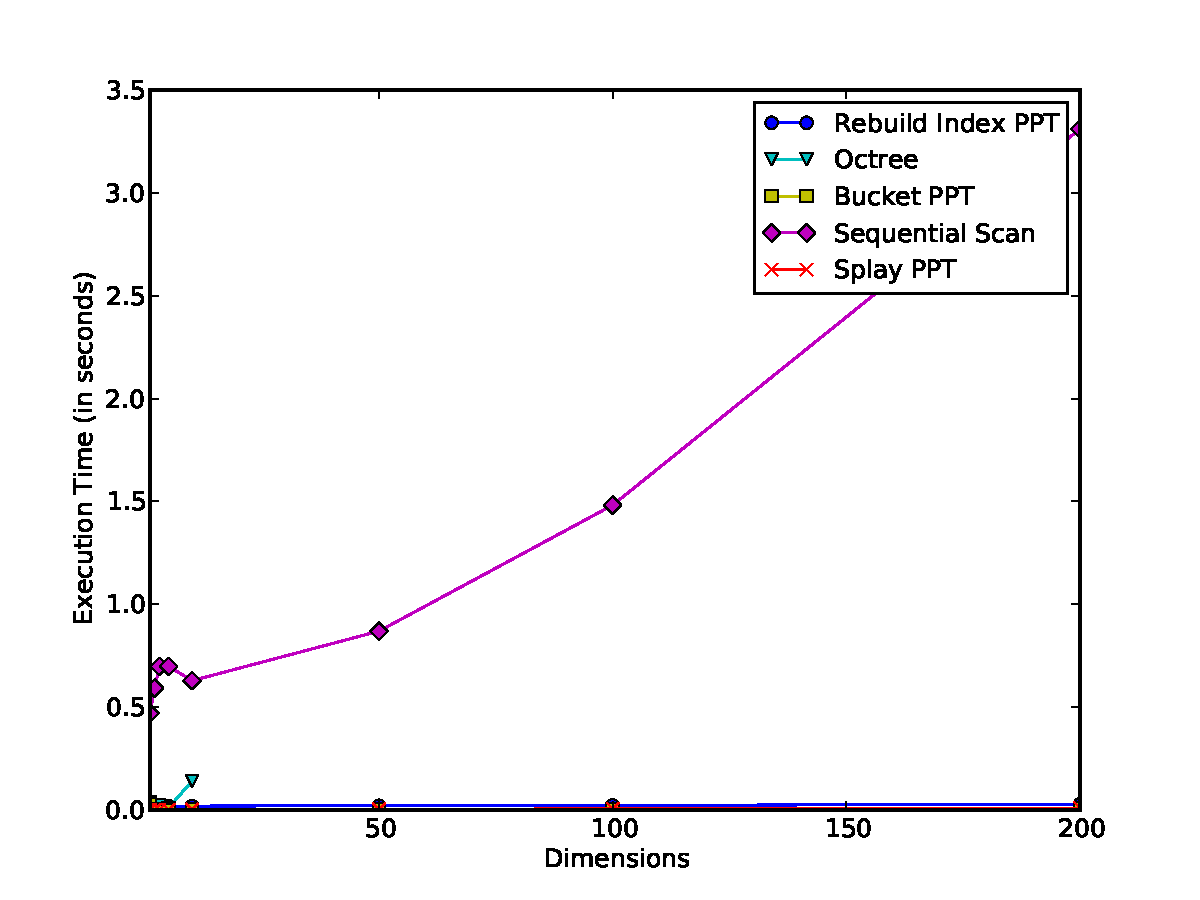
\includegraphics[scale=0.5]{figures/performance_analysis/iteration_1/randuniform_delete.pdf}
		}
		\end{subfloat}
	}%

	\caption{Index Structure Performance With Respect To Dimensionality (10,000 Points from Uniform Distribution Synthetic Dataset)}
	\label{fig:perf1-dimensionality}
\end{figure}

The three plots show that dimensionality has little effect on \textit{insert} and point queries for Sequential Scan. \texttt{delete}'s execution time increases as $d$ does, most likely because higher $d$ means more data has to be moved when a point is deleted from the underlying array. As expected, the Octree takes exponentially longer as $d$ increases, due to the exponential increase in nodes at each level ($2^d$ children per node). After 10 the number of excessive nodes was so high that the performance tests crashed due to there being no more memory to allocate.

All Pseudo-Pyramid Tree variants have similar speeds for \texttt{insert} and point queries, which significant outperforms Sequential Scan and Octree. However, the performance of the trees decreases as $d$ increases. The $O(n^2)$ defragmentation procedure used by the Defragmented Pseudo-Pyramid Tree causes it to be the slowest structure for deleting points, taking almost twice as long as Sequential Scan. Rebuild Pseudo-Pyramid tree is better, but still much slower than the Bucket or Splay Pseudo-Pyramid Tree variants, which have the fastest deletion speed. This is because TODO.

\begin{figure}
	\makebox[\textwidth][c]{%
		\begin{subfloat}[\texttt{insert}\label{fig:perf1-size-insert}]{%
			\begin{overpic}[scale=0.5]{figures/performance_analysis/iteration_1/sizevary_insert.pdf}
				\put(13,33){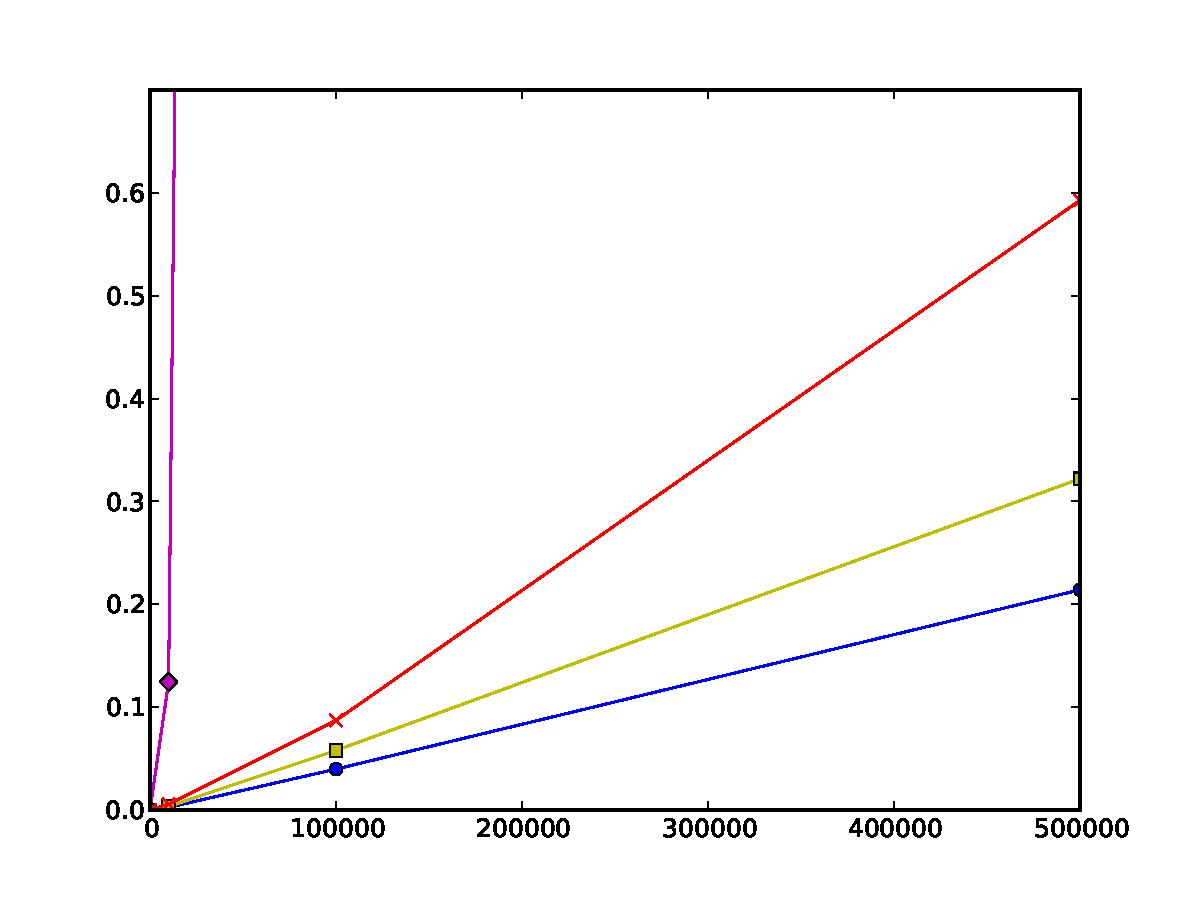
\includegraphics[scale=0.22]{figures/performance_analysis/iteration_1/sizevary_insert_zoomed.pdf}}
				\put(24,31){\textbf{\sans{Zoomed View}}}
			\end{overpic}
		}
		\end{subfloat}
		\begin{subfloat}[\texttt{delete}\label{fig:perf1-size-remove}]{%
			\begin{overpic}[scale=0.5]{figures/performance_analysis/iteration_1/sizevary_delete.pdf}
				\put(13,35){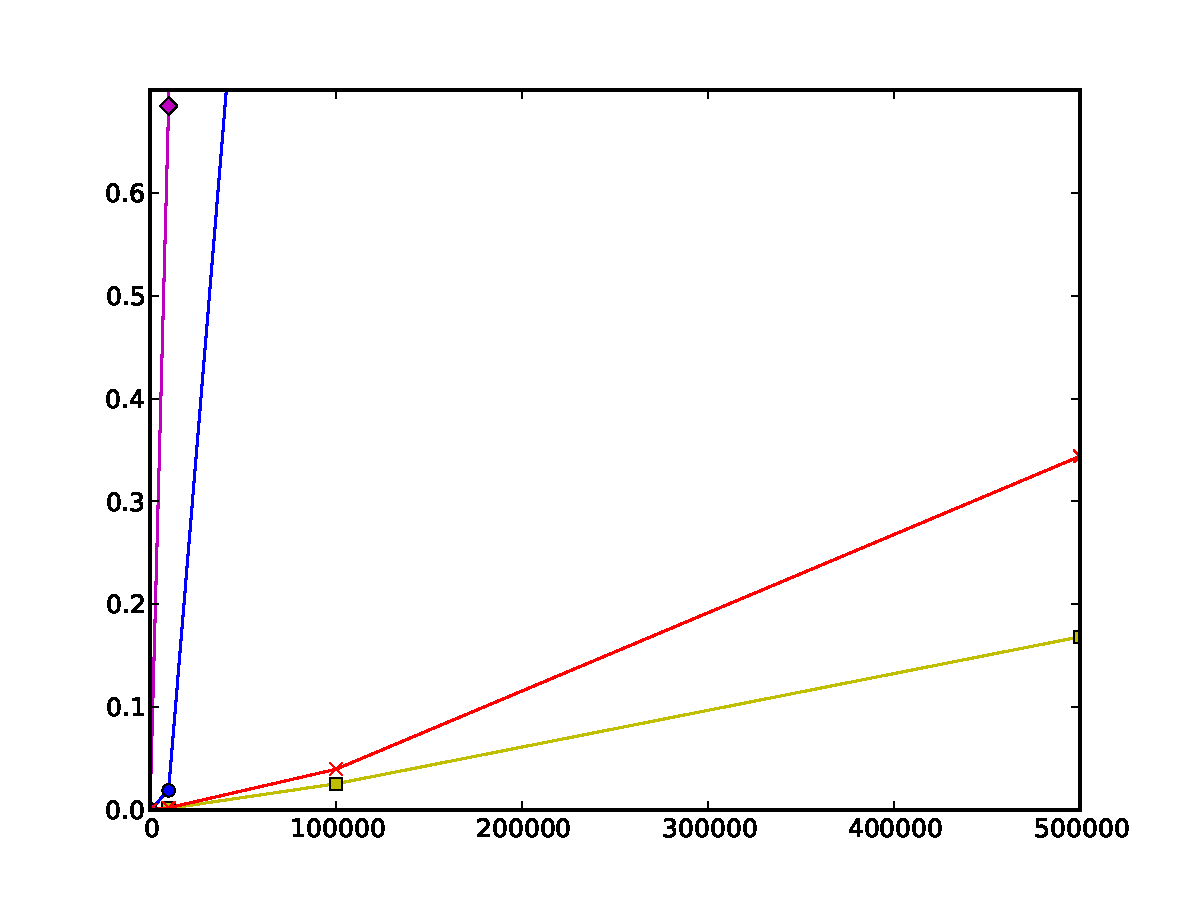
\includegraphics[scale=0.21]{figures/performance_analysis/iteration_1/sizevary_delete_zoomed.pdf}}
				\put(23,33){\textbf{\sans{Zoomed View}}}
			\end{overpic}
		}

		\end{subfloat}
	}%

	\caption{Index Structure Performance With Respect To Dataset Size (10,000 Points from Uniform Distribution Synthetic Dataset)}
	\label{fig:perf1-size}
\end{figure}

Execution times for the 16 dimension dataset of varying size are displayed in Table \ref{tab:perf1-size} and Figure \ref{fig:perf1-size}. From the plots, it appears the average time it takes to perform a point query and the other operations for Sequential Scan roughly grows linearly with $n$. This is to be expected, due to the complexity of its operations being $O(n)$. The average time for both operations with the Pseudo-Pyramid Tree variants grow very slowly as $n$ increases. This is likely because an operation's average complexity is $O(d)$ and dataset size only affects the performance of these operations if the tree's buckets become crowded with many points (as the buckets have to be searched to find the point).

\texttt{delete} in the Defragmented and Rebuild Pseudo-Pyramid Trees grow rapidly as $n$ is increased. Despite the defragmentation procedure being $O(n^2)$, the operation's execution appears to have linear growth (albeit with a higher constant factor than Sequential Scan). Perhaps this worst case bound was simply not reached in the tests, or there is some compiler optimisation at work which reduces this complexity.

Storing separate point arrays for each bucket, instead of using one large array to store all the points, can increase performance. This is shown by the bucket and splay variants providing faster \texttt{insert} and point query operations than the index-based variants. As expected, this is due to an increased cache hit rate. Table \ref{tab:perf1-cache-hit-rate} displays the cache miss rate (rounded to 2 decimal places) for each Pseudo-Pyramid Tree implementation. Notice how the two implementations which store indices in buckets have a greater cache miss rate. 

\begin{table}
	\centering
	\begin{tabular}{|l|l|}
		\hline
		\textbf{Structure} & \textbf{Cache Miss Rate (\%)} \\
		\hline
		Rebuild Pseudo-Pyramid Tree & 4.65 \\
		Bucket Pseudo-Pyramid Tree & 0.13 \\
		Splay Pseudo-Pyramid Tree & 0.29 \\
		\hline
	\end{tabular}
	\caption{Cache Hit Rate for \texttt{insert} Operations with Pseudo-Pyramid Variants (200D Randomly Uniform Dataset, 10,000 operations each)}
	\label{tab:perf1-cache-hit-rate}
\end{table}

The differences in speed between the bucket and splay variants is small, but the Bucket Pseudo-Pyramid Tree outperforms the Splay Tree with most datasets. Again, this may be due to having a lower cache miss rate. With severely skewed synthetic data, the splay variant is \textit{slightly} faster, but the speed increase is negligible. This could be an indication that self-adjusting structures are useful for heavily skewed data however, highlighting an area for further study. TODO: refer to table

TODO: sort out delete being so much faster???

\begin{table}
	\centering
	\makebox[\textwidth][c]{%
		\begin{tabular}{|r|r|l|l|l|}
			\hline
			\multicolumn{2}{|c}{} & \multicolumn{3}{|c|}{\textbf{Dataset}} \\
			\hline
			\textbf{Structure} & \textbf{Operation} & \textbf{Astrophysics} & \textbf{Hurricane Isabel} & \textbf{Armadillo Mesh} \\
			\hline
			\multirow{4}{*}{Sequential Scan} & Delete & 1315.81 & 1920.73 & TODO \\
				& Insert & 436.385 & 691.833 & TODO \\
				& Point Query & 435.88 & 651.428 & TODO \\
			\hline
			\multirow{4}{*}{Rebuild Index PPT} & Delete & 1856.11 & 2121.9 & TODO \\
				& Insert & 139.346 & 117.441 & TODO \\
				& Point Query & 139.048 & 117.292 & TODO \\
			\hline
			\multirow{4}{*}{Bucket PPT} & Delete & 41.8115 & 34.8281 & TODO \\
				& Insert & 81.231 & 69.401 & TODO \\
				& Point Query & 70.4391 & 69.3368 & TODO \\
			\hline
			\multirow{4}{*}{Splay PPT} & Delete & 44.0876 & 34.8037 & TODO \\
				& Insert & 84.0908 & 69.5318 & TODO \\
				& Point Query & 70.3729 & 69.3996 & TODO \\
			\hline
		\end{tabular}
	}%

	\caption{Total Execution Time (in seconds) of Each Operation on Sampled Real Datasets}
	\label{tab:perf1-real}
\end{table}

Table \ref{tab:perf1-real} shows the runtime of each operation on the real evaluation datasets, measured using the Insert-Query-Delete operation list.TODO: remarks on it

\subsection{Profiling Results}

CPU and heap profiling was performed on each structure to determine where the performance bottlenecks are and how much memory each structure uses. Table \ref{fig:perf1-profiling} shows which functions took the majority of the execution time for each structure, as well as how much heap memory the structure consumed when storing all of the input dataset's points. The dataset used contained 10,000 10D uniformly random points and the CPU profiling was performed over the Insert-Query-Delete operation list.

\begin{table}
	\centering
	\makebox[\textwidth][c]{%
		\begin{tabular}{|l|l|l|}
			\hline
			\textbf{Structure} & \textbf{Peak Heap Memory (MB)} & \textbf{Dominant Function (\% Total Time Spent)} \\
			\hline
			Sequential Scan & 4.1 & \texttt{pointExists()} (34.4\%) \\
			Defragmented PPT & 10.9 & \texttt{defragment()} (76.6\%)\\
			Rebuild PPT & 16.8 & \texttt{rebuild()} (60.7\%)\\
			Bucket PPT & 11.2 & \texttt{remove()} (19.2\%) \\
			Splay PPT & 11.8 & \texttt{insert()} (47.2\%) \\
			\hline
		\end{tabular}
	}%
	\caption{CPU and Heap Profiling Statistics for Insert-Query Delete Operation List with 500,000 Points from 16D Synthetic Dataset}
	\label{tab:perf1-profiling}
\end{table}

TODO: analysis

\subsection{Impact of Bucket Size}

Work gone into increasing the speed of the Pseudo-Pyramid Tree by exploring different variants of the structure's implementation. This has worked to greatly accelerate the structure for most of the evaluation datasets. However, when testing on the astrophysics dataset, the speedup when compared to Sequential Scan seemed to be quite low. For example, $500,000$ insertion operations with the astrophysics dataset takes TODO seconds with Sequential Scan and TODO seconds with the Bucket Pseudo-Pyramid Tree, meaning a speedup of $\frac{TODO}{TODO} \approx TODO$ has been achieved. Considering there exist algorithms which can perform search in $O(log_2 n)$ time, this raised the question of why the speedup is so low for the astrophysics dataset.

Despite hashing a point taking $O(d)$ time, point queries will take much longer if there are large numbers of points in buckets. If each bucket contains exactly one point, then the complexity approaches $O(d)$. On the other extreme, where a single bucket contains all points, the complexity becomes $O(n)$. The number of points in a bucket, or \textit{bucket size}, is one of the most important factors to consider when analysing the performance of hash-based index structures. A ``good" hashing function tries to achieve an amortised running time of $O(1)$ by ensuring only one or two points are mapped to the same hash value.

The mean, standard deviation, minimum and maximum bucket size has been used to determine if bucket size is the reason the Pseudo-Pyramid Tree is so slow for the astrophysics dataset. Table \ref{tab:perf1-bucket-stats} shows these statistics when the Pseudo-Pyramid Tree is storing points from one synthetic dataset and all the real datasets.

\begin{table}
	\centering
	\begin{tabular}{|l|l|l|l|l|l|}
		\hline
		& & \multicolumn{4}{c|}{\textbf{Bucket Size Statistics}} \\
		\hline
		\textbf{Dataset} & \textbf{Time to Insert (sec)} & \textbf{Average} & \textbf{St. Dev} & \textbf{Min} & \textbf{Max} \\
		\hline
		500,000 16D Random Points & TODO & 1.0312 & 0.115177 & 1 & 4 \\
		500,000 Astrophysics Points & TODO & 3586.57 & 24,528 & 1 & 235,260 \\
		500,000 Hurricane Isabel Points & TODO & 17,323.66 & 83,533 & 1 & 293,949 \\
		435,544 3D Armadillo Mesh Points & TODO & 19.1465 & 14.9386 & 1 & 187 \\
		\hline
	\end{tabular}
	\caption{Statistics on Bucket Size with Pseudo-Pyramid Tree Based on Dataset}
	\label{tab:perf1-bucket-stats}
\end{table}

TODO: remarks on stats in above table

TODO: why is bucket size so high????????????

\subsection{Summary}

All Pseudo-Pyramid tree invariants greatly outperform the two baselines, with the Octree failing to store large numbers of points or points with more than 10 dimensions due to exponential memory requirements. The defragmented and rebuild variants of the Pseudo-Pyramid are clearly inferior to batch and splay, being slower for all three operations. While the Splay Pseudo-Pyramid Tree performs the fastest for some datasets, the Bucket Pseudo-Pyramid Tree performs the fastest on the majority of the datasets. Therefore, the Bucket Pseudo-Pyramid Tree will be used for any future evaluations.

With both scientific datasets, all Pseudo-Pyramid Tree variants degenerated to semi-sequential scan because of the dataset's point distribution. To determine whether or not hash-based index structures can provide fast point queries for scientific datasets such as the astrophysics and hurricane Isabel simulations, more research into decreasing bucket size by using different hashing functions should be performed, which is the focus of the next iteration.
\section{Iteration \#2 -- Pyramid Tree and Other Hash-Based Approaches}

This iteration explores other hashing functions to find a hash-based index structure which performs well on the two scientific datasets.

\subsection{Pyramid Tree}

TODO: using same underlying implementation w/ optimisations as Pseudo-Pyramid Tree -- just hashing function that's changed!

\subsection{B${}^+$-Tree as Underlying Structure}

Berchtold et al. originally used a B${}^{+}$-tree when developing the Pyramid Tree \cite{pyramid-tree}. It was decided that using the same underlying search structure would allow for a more fair comparison of the Pyramid tree data structure. Two B${}^{+}$-tree implementations, cpp-btree\cite{cpp-btree} and bpt\cite{bpt}, were plugged and tested into the Pyramid Tree. The first is a C++ implementation while the second is a pure C implementation.

Table \ref{tab:hashtable-bplus-time-comparison} provides timings for a single synthetic dataset. There is a substantial difference between the speed of the hash table Pyramid tree and the B${}^{+}$-tree implementations. After profiling, it was discovered the main cause of the decrease in speed was simply the additional overhead incurred by splitting and merging nodes in the B${}^{+}$-tree. This matches the theoretical performance analyses of the two structures, where it is shown that hash tables and B${}^{+}$-trees have amortised $O(1)$ and $O(\log n)$ operations respectively (the former being dependant on the hashing function used).

Based on these results, it has been decided to continue using the hash table and the underlying search structure, and not the B${}^{+}$-tree.

\begin{table}
	\centering
	\begin{tabular}{|l|l|l|l|}
		\hline
		\textbf{Operation} & \texttt{boost::unordered\_map} & cpp-btree & bpt \\
		\hline
		\textbf{Insert} & TODO & TODO & TODO \\
		\textbf{Delete} & TODO & TODO & TODO \\
		\textbf{Point Query} & TODO & TODO & TODO \\
		\hline
	\end{tabular}
	\caption{Total Execution Time (in Seconds) of Batch Pseudo-Pyramid Tree With Different Underlying 1D Index Structures (200D Randomly Uniform Dataset, 10,000 operations each)}
	\label{tab:hashtable-bplus-time-comparison}
\end{table}

\subsection{Bucket Hash Table}

% http://stackoverflow.com/questions/7403210/hashing-floating-point-values
% https://svn.boost.org/trac/boost/ticket/4038
% http://programmers.stackexchange.com/questions/63595/0x9e3779b9-golden-number
% http://stackoverflow.com/questions/4948780/magic-number-in-boosthash-combine
% http://burtleburtle.net/bob/hash/doobs.html

If larger bucket sizes mean more point comparisons are performed on average, then it is not unreasonable to expect an average bucket size of 1 to provide very good performance. After all, if the hashing function is an $O(d)$ operation, then it follows that \texttt{insert}, \texttt{delete} and point query operations take $O(d)$ time. 

The Bucket Hash Table also uses a \texttt{boost::unordered\_map} in the back-end, but instead of trying to exploit the spatial properties of points directly to provide good bucket size, a different, more general-purpose hashing function provided in the Boost library is used. Like the other hash-based structures discussed in this section, it is possible for two points to be hashed to the same value. However, from empirical performance tests, it has been shown that the average bucket size is almost always near one (bucket size measurements are provided in the next section), meaning most operations are performed in $O(d)$ time.

A high-level algorithm describing the hashing function is given in Algorithm \ref{alg:point-hashing} in Appendix \ref{chap:supp-material}. This function hashes each individual coordinate (floating point value) and combines them using exclusive-or ($\oplus$) and bitshifting operations. A magic number representing the reciprocal of the golden ratio, $\phi = \frac{1 + \sqrt{5}}{2}$, is used when combining the hash values of individual coordinates. The choice to use the golden ratio was inspired by Jenkins' hash function\cite{hash-combine}, where it is used to ensure consecutive floating point values will be mapped to integers with large distances between them. This increases the likelihood of having points distributed more uniformly across buckets when points are clustered within a small numerical range (like they are in the astrophysics dataset).

One major issue with this approach is the potential for floating-point inaccuracy to give incorrect results. On the controlled performance tests executed in this project, a point is queried using the exact same floating point values for the coordinates as when it was inserted. This means the two points have the same identical bit patterns. 

Suppose the point to query was the output of a more complex computation, where rounding errors may come into play. Even if an equal point conceptually is being stored in the structure, rounding errors may cause the two points to have different bit patterns, potentially resulting in different hashed values. The output point, while being stored in the structure, will appear as if it is not. This is a common issue when using floating point values in hashing functions.

Therefore, the Bucket Hash Table may be unreliable for certain applications, especially ones where the input points are the result of computations involving many arithmetic operations.

\subsection{Bucket Statistics}

The same underlying implementation is used for the Pseudo-Pyramid Tree, Pyramid Tree and Bucket Hash Table; only the hashing function varies. Pyramid Tree's and Bucket Hash Table's hash functions have also been parallelised using SSE, which has made the difference between execution times between the hash functions of the three structures very small. The core factor which determines the performance of each structure is still bucket size. Therefore, statistics on the bucket size will be used to determine which structure is superior. As in iteration one, one synthetic dataset and all three real datasets will be used for bucket size measurement.

\begin{table}
	\centering
	\begin{tabular}{|l|l|l|l|l|}
		\hline
		\textbf{} & \multicolumn{4}{c|}{\textbf{Bucket Size Statistics}} \\
		\hline
		\textbf{Dataset} & \textbf{Average} & \textbf{St. Dev} & \textbf{Min} & \textbf{Max} \\
		\hline
		\textbf{Pseudo-Pyramid Tree} & & & & \\
		500,000 16D Random Points & TODO & TODO & TODO & TODO \\
		500,000 Astrophysics Points & TODO & TODO & TODO & TODO \\
		500,000 Hurricane Isabel Points & TODO & TODO & TODO & TODO \\
		435,544 3D Armadillo Mesh Points & TODO & TODO & TODO & TODO \\
		\hline
		\textbf{Pyramid Tree} & & & & \\
		500,000 16D Random Points & TODO & TODO & TODO & TODO \\
		500,000 Astrophysics Points & TODO & TODO & TODO & TODO \\
		500,000 Hurricane Isabel Points & TODO & TODO & TODO & TODO \\
		435,544 3D Armadillo Mesh Points & TODO & TODO & TODO & TODO \\
		\hline
		\textbf{Bucket Hash Table} & & & & \\
		500,000 16D Random Points & TODO & TODO & TODO & TODO \\
		500,000 Astrophysics Points & TODO & TODO & TODO & TODO \\
		500,000 Hurricane Isabel Points & TODO & TODO & TODO & TODO \\
		435,544 3D Armadillo Mesh Points & TODO & TODO & TODO & TODO \\
		\hline
	\end{tabular}
	\caption{Statistics on Bucket Size, Based on Dataset, of All Hash-Based Structures}
	\label{tab:perf2-bucket-stats}
\end{table}

Table \ref{tab:perf2-bucket-stats} contains statistics on bucket size for all three hashing functions. TODO: discussion of results and implications

\subsection{Summary}

TODO


\chapter{Technical Evaluation}
\label{chap:technical-evaluation}
\centerline{\rule{149mm}{.02in}}
\vspace{2cm}

We have shown that the point $kd$-tree greatly outperforms the Pyramid tree for the two scientific datasets. For all synthetic data and the 3D point cloud dataset, the Pyramid tree is faster, especially with point deletion. This chapter will explore the reasons for this, determining what properties the astrophysics dataset has which cause the performance of the structures to degenerate. The chapter will conclude by discussing the types of data suitable for the Pyramid Tree and $kd$-tree, along with some further discussion on the implications of the results from this evaluation.

\section{Characteristics of Astrophysics Dataset}
\label{sec:data-characteristics}

A dataset can be considered \textit{skewed} if there are more points in some regions of the data space than other regions. In other words, the underlying frequency or probability distribution of point locations is non-uniform. Intuitively, the skewness of a dataset increases as the \textit{difference} between the frequency, or probability, of points in different spatial regions increases.

Histograms are used to visualise the frequency distributions of one-dimensional data. Since this project deals with multi-dimensional data, multiple histograms, one for each dimension, can be produced to gain insight into point distribution. The astrophysics dataset was computed using a 3D sampling lattice, computing ten fields at each point. The original simulation uses interpolation to compute the ten fields at each point on the lattice \cite{astrophysics-dataset}. Carr et al. discusses how this interpolation ``implicitly applies the spatial relation between sample points" and shows that histograms are equivalent to nearest-neighbour interpolation \cite{histograms-and-isosurfaces}. This means histograms poorly represent datasets that use higher-order interpolants, such as the astrophysics dataset, because they ``over-emphasizes densely-sampled regions and under-emphasizes sparsely-sampled regions" \cite{histograms-and-isosurfaces}. 

Isosurface statistics have been proposed as a superior representation of such datasets \cite{histograms-and-isosurfaces}. They are conceptually and computationally more complex to compute however. Due to the project's time constraints, isosurface statistics will not be used. While histograms are poorer representation of the data, the aim of this evaluation is to get an approximation of the magnitude of the astrophysics dataset's skew. Histograms still allow for this even if they are not as accurate as other techniques. As such, histograms will be used to visualise the distribution of the astrophysics dataset.

\begin{figure}
	\begin{center}
		\begin{subfloat}[Dimension 1 (total particle density)]{%
			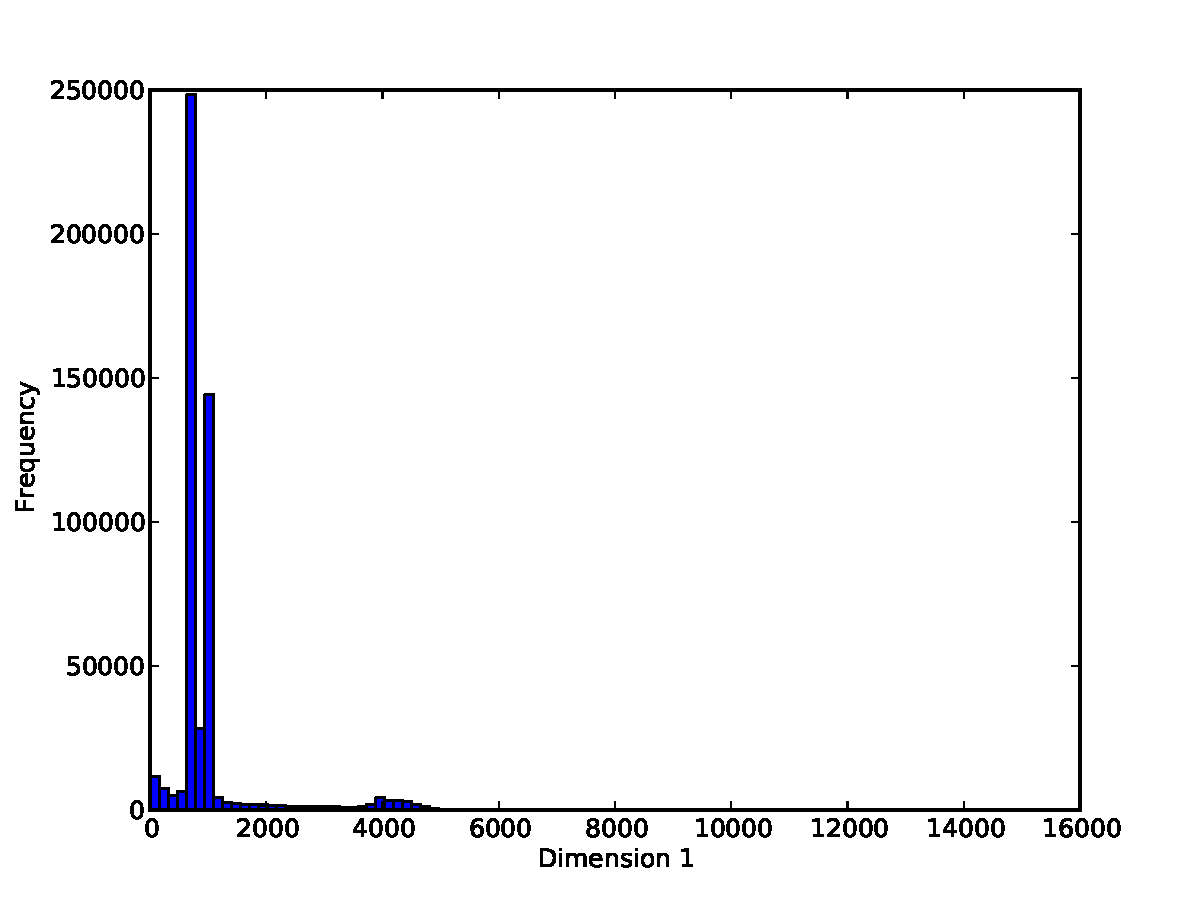
\includegraphics[scale=0.36]{figures/histograms/astrophysics_500000_0.pdf}
		}
		\end{subfloat}~
		\begin{subfloat}[Dimension 2 (gas temperature)]{%
			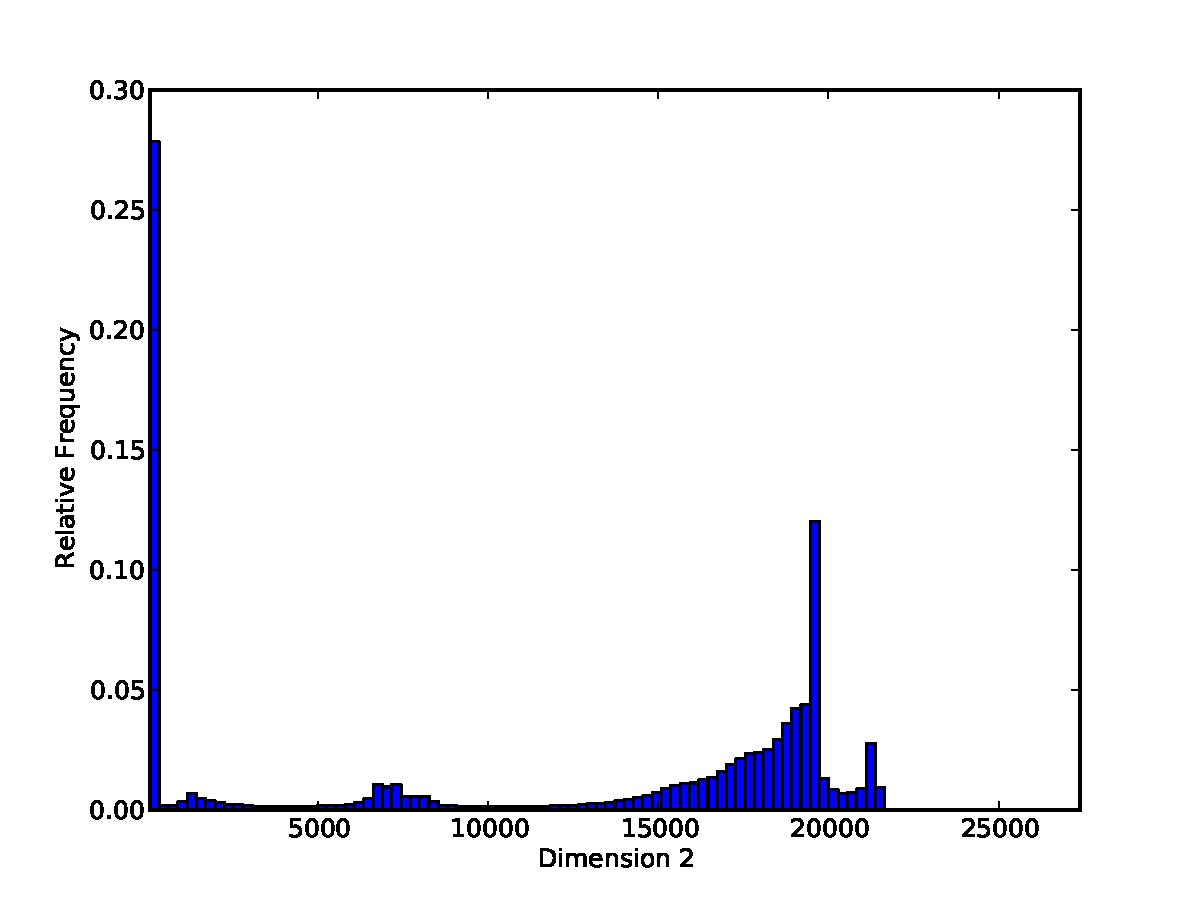
\includegraphics[scale=0.36]{figures/histograms/astrophysics_500000_1.pdf}
		}
		\end{subfloat}
	\end{center}

	\caption{Frequency Distributions of Dimensions 1 and 2 of Astrophysics Dataset}
	\label{fig:astrophysics-histograms1}
\end{figure}

\begin{figure}
	\begin{center}
		\begin{subfloat}[Dimension 3 (H mass abundance)]{%
			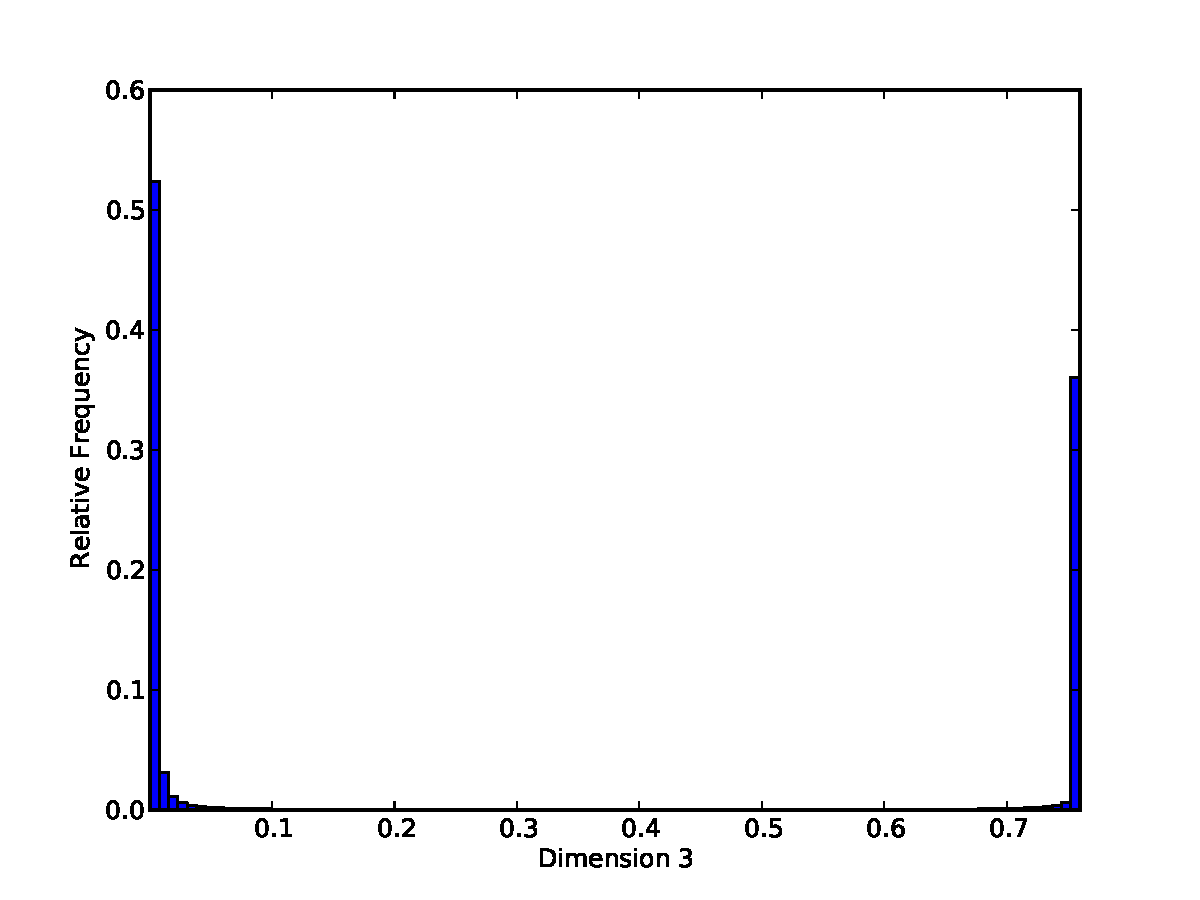
\includegraphics[scale=0.36]{figures/histograms/astrophysics_500000_2.pdf}
		}
		\end{subfloat}~
		\begin{subfloat}[Dimension 7 (He${}^{++}$ mass abundance)]{%
			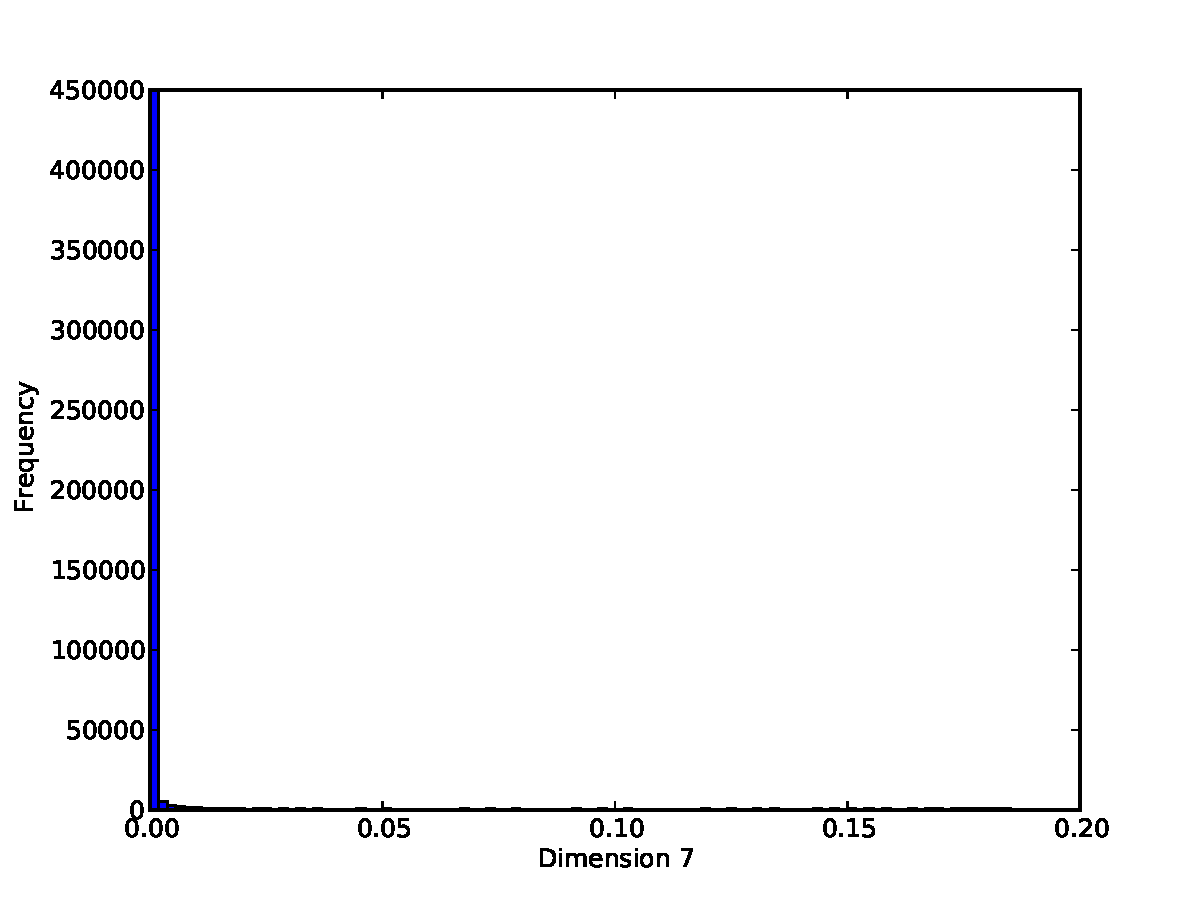
\includegraphics[scale=0.36]{figures/histograms/astrophysics_500000_6.pdf}
		}
		\end{subfloat}
	\end{center}

	\caption{Frequency Distributions of Dimensions 3 and 7 of Astrophysics Dataset}
	\label{fig:astrophysics-histograms2}
\end{figure}

Using the same sampled astrophysics dataset used for performance analysis in Chapter \ref{chap:design-and-implementation}, a histogram has been generated for each of the ten dimensions. Figures \ref{fig:astrophysics-histograms1} and \ref{fig:astrophysics-histograms2} show histograms of dimensions 1, 2, 3 and 7. The remaining dimensions have distributions similar to the dimensions shown here, so they add little value to the discussion. They can be found in Appendix \ref{sec:app-histograms} for completeness. Using these histograms, the following observations can be made:
\begin{enumerate}
	\item the first two dimensions, total particle density and gas temperature, appear to have the greatest variance, although there are still very large peaks
	\item most points are clustered on the lower or upper boundaries of dimensions 3, 4, 5 and 6. The respective histograms have massive peaks at either end of the distribution and much smaller peaks in between
	\item most points are clustered on the lower boundary of dimensions 7, 8, 9 and 10, with a single large peak on the histograms
\end{enumerate}
The astrophysics dataset is therefore highly skewed, since most points are clustered at the boundaries of each dimension. It follows that the vast majority of the data space has little to no points, making the data space \textit{sparse}.

\section{Effect of Distribution on Pyramid Tree}

We now explore the effect of the highly skewed distribution on the Pyramid Tree. Recall that the Pyramid Tree maps a point $v$ to a single scalar named the Pyramid value $pv_v$. Points with the same Pyramid value are stored in the same bucket. Table \ref{tab:final-bucket-size} shows bucket size statistics and how long it takes to query all the points for the sampled astrophysics dataset with different subsets of dimensions. When only dimensions 1 and 2, the dimensions with the greatest variance, are used, average bucket size decreases substantially. Dimensions 3 and 7 have larger clusters of points close together, so they cause the average bucket size to increase.

The histograms from Section \ref{sec:data-characteristics} illustrate how most points lie on, or close to, the boundaries of the dataset. This is a significant problem for the Pyramid Tree because it always chooses the dimension whose distance from the centre point of the data is the highest. If a large number of points are on a dimensional boundary, then its likely the same dimension will be chosen. Each point will the same coordinate value for the chosen dimension because they are on the same boundary, meaning will have the same pyramid value and will be mapped to the same bucket.

\begin{table}
	\centering
	\makebox[\textwidth][c]{%
		\begin{tabular}{|l|l|l|l|l|}
			\hline
			\textbf{Dimensions} & \textbf{Time to Query (sec)} & \textbf{Average} & \textbf{Max} & \textbf{\#Buckets} \\
			\hline
			All & 60.0216 & 3586.57 & 235260 & 120 \\
			1 and 2 & 0.0713558 & 6.52433 & 102 & 25232 \\
			3 and 7 & 8.30587 & 89.2853 & 141235 & 3056 \\
			\hline
			No Boundary Coordinates & 27.6034 & 25.3722 & 45031 & 16963 \\
			\hline
		\end{tabular}
	}%
	\caption{Pyramid Tree Bucket Size Statistics with Different Dimensions of Astrophysics Dataset}
	\label{tab:final-bucket-size}
\end{table}

Histograms are equivalent to nearest-neighbour interpolation, so they do not show if the points inside the bins at the boundary of the graphs are \textit{actually} boundary values or just close to the boundary. To determine if clusters of points at boundaries is truly the main cause of large buckets, a heuristic called \textbf{No Boundary Coordinates} was developed. Let $v$ be a point and $min_i$ and $max_i$ be the minimum and maximum boundary values for dimension $i \in \lbrace 0, 1, ..., d - 1 \rbrace$. Let $j$ be the dimension $v$ is furthest away from the centre point with. If $v_j = min_j$ or $v_j = max_j$, then a new dimension $k$ is chosen, such that $v_k$ is the \textit{second} furthest coordinate from the centre point. If $v_k$ is at the boundary, then the next furthest is chosen. This process is repeated until a coordinate which is not on a boundary is found. If all coordinates are on a boundary, then the first dimension is chosen.

Table \ref{tab:final-bucket-size} shows how this simple heuristic decreases average bucket size. However, it is still significantly slower than the $kd$-tree, so other kinds of skew are still causing problems. One could apply further heuristics in an attempt to improve Pyramid Tree performance on the astrophysics dataset, but it is likely that the structure will start overfitting the dataset and performing worse on other datasets. Creating heurstics like this requires pre-existing knowledge of the dataset's distribution, which may not be available, especially when the data dynamic (i.e. it is not \textit{possible} to know all the data in advance).

\section{Effect of Distribution on $kd$-tree}

For completeness, different dimensions of the astrophysics dataset were also tested on the point $kd$-tree. Table \ref{tab:final-balance-factor} shows the query time, balance factor and maximum path length of the tree with these different dimensions. It can be observed that the point $kd$-tree, like the Pyramid Tree, performs worse because of the skew present in the astrophysics dataset as well. Using dimensions 1 and 2 gives a lower balance factor than the more skewed dimensions 3 and 7. The difference in performance between the chosen dimensions is much smaller than the Pyramid tree, however, again showing the point $kd$-tree is more resilient to skew.

\begin{table}
	\centering
	\makebox[\textwidth][c]{%
		\begin{tabular}{|l|l|l|l|l|}
			\hline
			\textbf{Dimensions} & \textbf{Time to Query (sec)}  & \textbf{Balance Factor} & \textbf{Max Path Length}  \\
			\hline
			All & 0.639265 & 32.405 & 120 \\
			1 and 2 & 0.18445 & 26.5923 & 73 \\
			3 and 7 & 0.257211 & 28.6481 & 69 \\
			\hline
		\end{tabular}
	}%
	\caption{Point $kd$-tree Statistics with Different Dimensions of Astrophysics Dataset}
	\label{tab:final-balance-factor}
\end{table}

\section{Conjecture on Scientific Datasets}

While an analysis of the hurricane Isabel dataset is not in this report, generating histograms of each dimension reveals distributions similar to the astrophysics dataset. Some dimensions have smoother distributions, whereas others contain large clusters of points at the boundaries. This raises an important question: do datasets resulting from scientific simulations generally have these properties, or are these properties just specific to these datasets? If the former is true, more general hypotheses can be made regarding the index structures that are suitable for scientific computation and visualisation.

Exploring the properties of scientific multi-dimensional datasets is a project in itself, so an in-depth analysis of such properties will not be performed. Instead, existing literature will be used as the basis for the following conjecture.

\paragraph{\textbf{CONJECTURE:}} Dense clusters of points and sparse regions of data space is a property present in the majority of scientific datasets computed using sampling lattices.
\paragraph{}

Scientific datasets are often computed using $m$-dimensional sampling lattices, where each point on the lattice represents a point in physical space \cite{TODO}. This means $m$ is usually 2 or 3. $d$ continuous fields are measured at each point, which are typically physical properties such as temperature, wind velocity, chemical masses and so on. Interpolation is applied in some way to model the spatial relationships between the properties of the sampling points in physical space.

It is common for $d$ to be larger than $n$, as is the case in the astrophysics and hurricane datasets. Such physical simulations can be described as a mapping $\mathbb{R}^n \rightarrow \mathbb{R}^d$, where $d > n$. A data space's volume increases exponentially as $d$ increases, resulting in sparsity, as discussed in Section \ref{sec:curse-of-dimensionality}). To fill the data space, an exponentially increasing number of data points must be sampled, which is not viable for high $d$.

Data sparsity becomes an even greater issue when mapping continuous domains to higher dimensional space because the resulting $d$-dimensional dataset becomes a sampled $m$-dimensional manifold in $d$-dimensional space \cite{TODO}. Figure \ref{fig:manifolds} illustrates examples of manifolds for $\mathbb{R}^1 \rightarrow \mathbb{R}^2$ and $\mathbb{R}^2 \rightarrow \mathbb{R}^3$. Notice how the majority of the data spaces in both examples are empty. Only thin strips of the data spaces are filled by the lower-dimensional manifolds. The astrophysics dataset was the result of a $\mathbb{R}^3 \rightarrow \mathbb{R}^{10}$ simulation, so a 3 dimensional manifold will be embedded in 10 dimensional space. This results in a highly sparse space, which may be one of the reasons there are so many large clusters of points in the astrophysics dataset.

\begin{figure}
	\begin{center}
		\begin{subfloat}[$\mathbb{R}^1 \rightarrow \mathbb{R}^2$]{%
			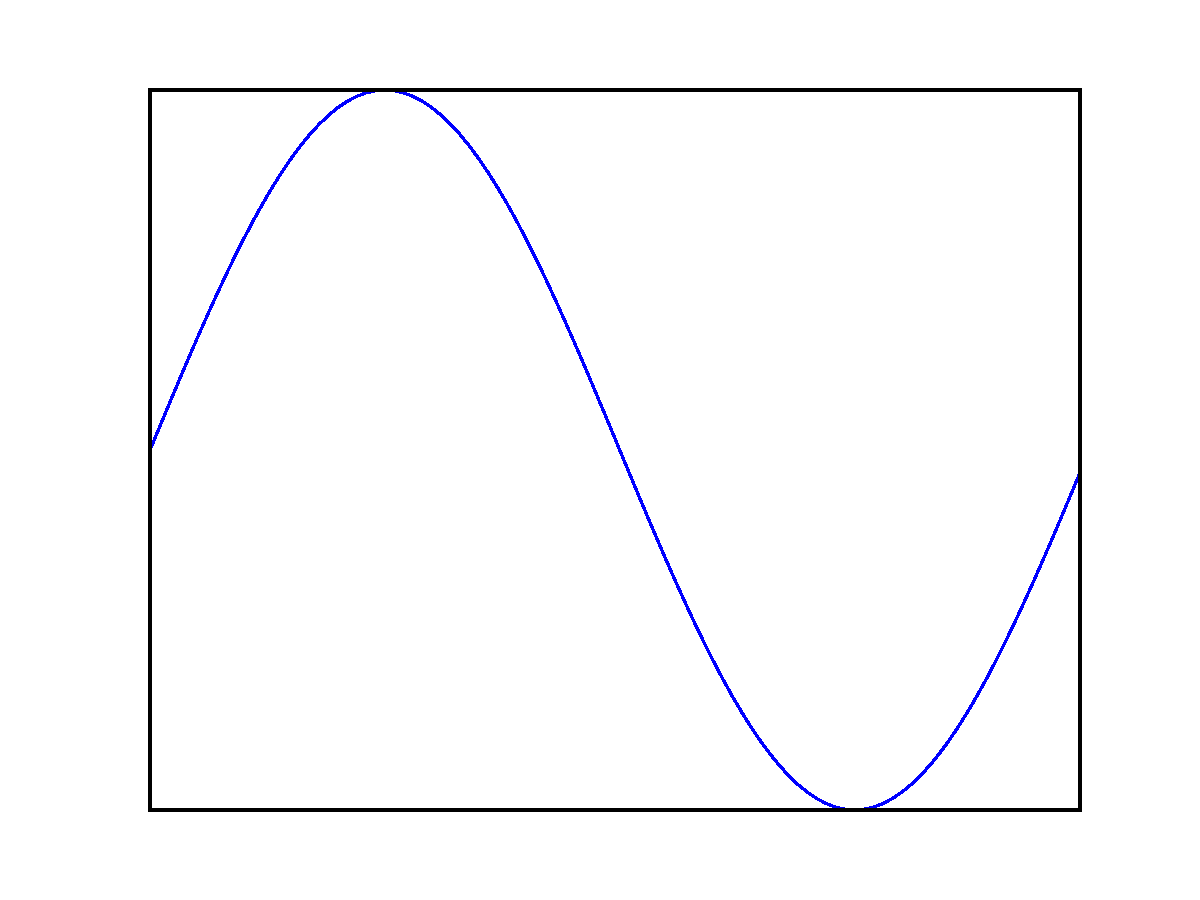
\includegraphics[scale=0.2]{figures/1d_manifold.pdf}
		}
		\end{subfloat}~
		\begin{subfloat}[$\mathbb{R}^2 \rightarrow \mathbb{R}^3$]{%
			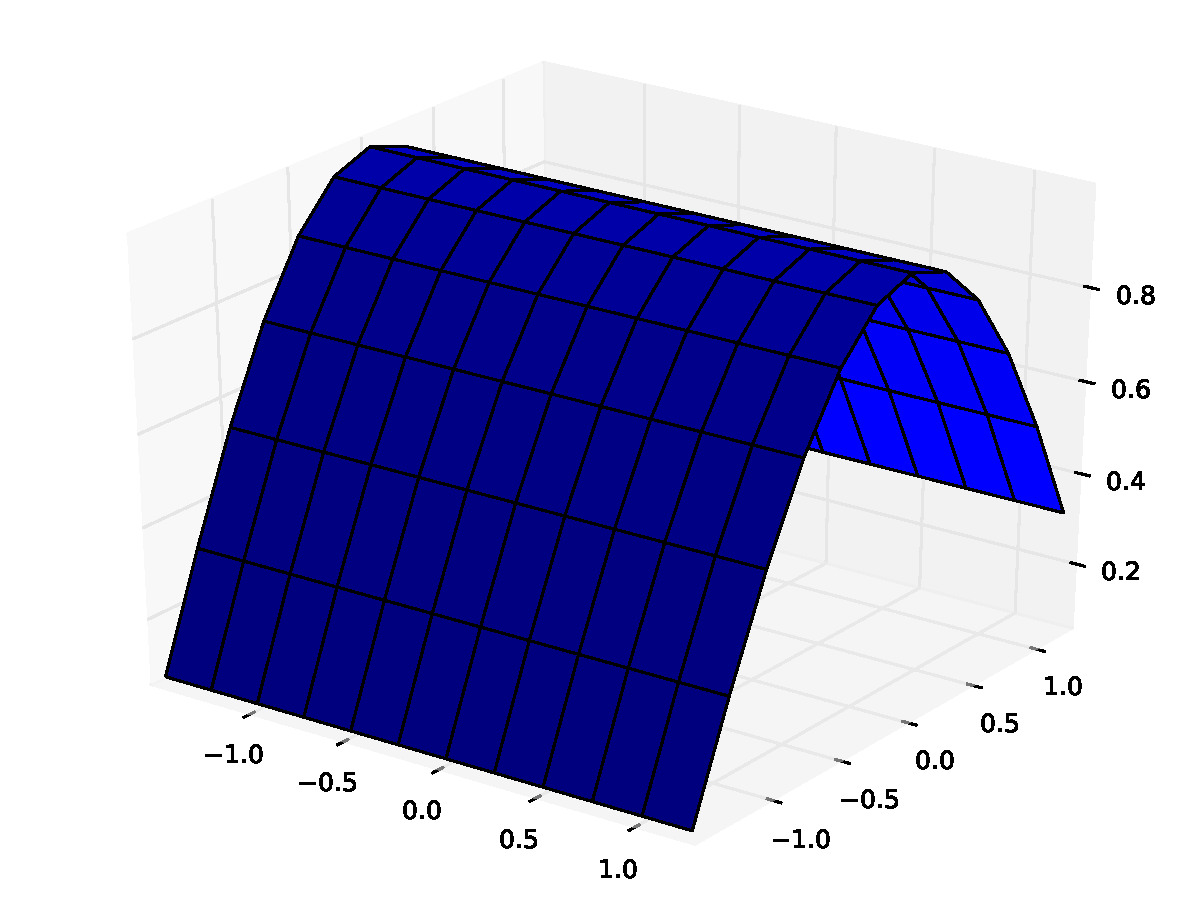
\includegraphics[scale=0.225]{figures/2d_manifold.pdf}
		}
		\end{subfloat}
	\end{center}

	\caption{Manifolds Embedded in Higher-Dimensional Space}
	\label{fig:manifolds}
\end{figure}

\section{Implications to Multi-dimensional Search}

Data sparsity becomes an issue for index structures which decompose the underlying data space. The Pyramid Tree uses a \textit{static} decomposition. Based on the initial boundary, exactly how the space is decomposed is determined. For some data, such as the synthetic data used in Chapter \ref{chap:design-and-implementaton}, this is not a problem. However, there cases where the lack of ability to \textit{adapt} the decomposition to the input data becomes problematic, which was the case with the astrophysics dataset since most points will be mapped to the same few buckets.

\begin{figure}
	\begin{center}
		\begin{subfloat}[Non-Continuous Embedding Decomposed with Pyramid Tree]{%
			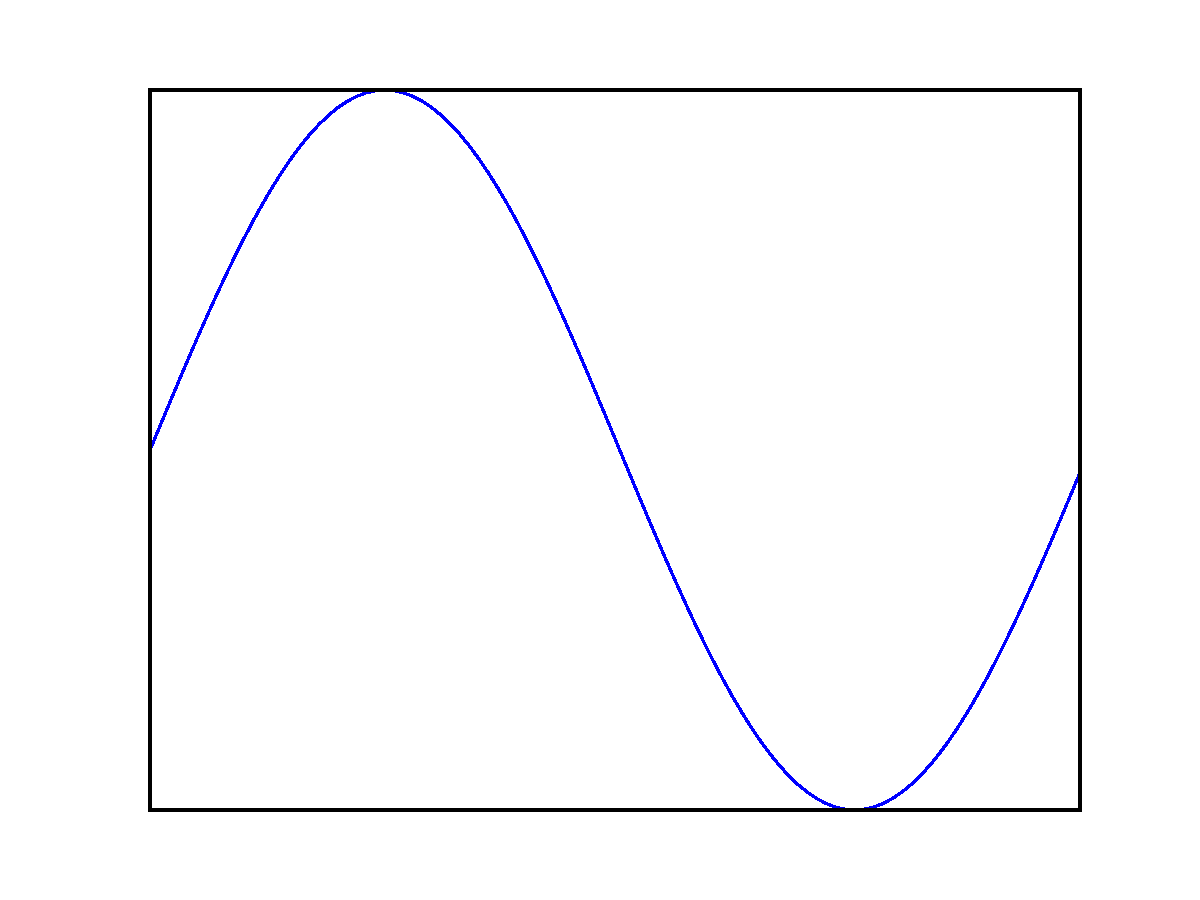
\includegraphics[scale=0.2]{figures/1d_manifold.pdf}%{figures/non-continuous-pyramid.pdf}
		}
		\end{subfloat}~
		\begin{subfloat}[Continuous Embedding Decomposed with Pyramid Tree]{%
			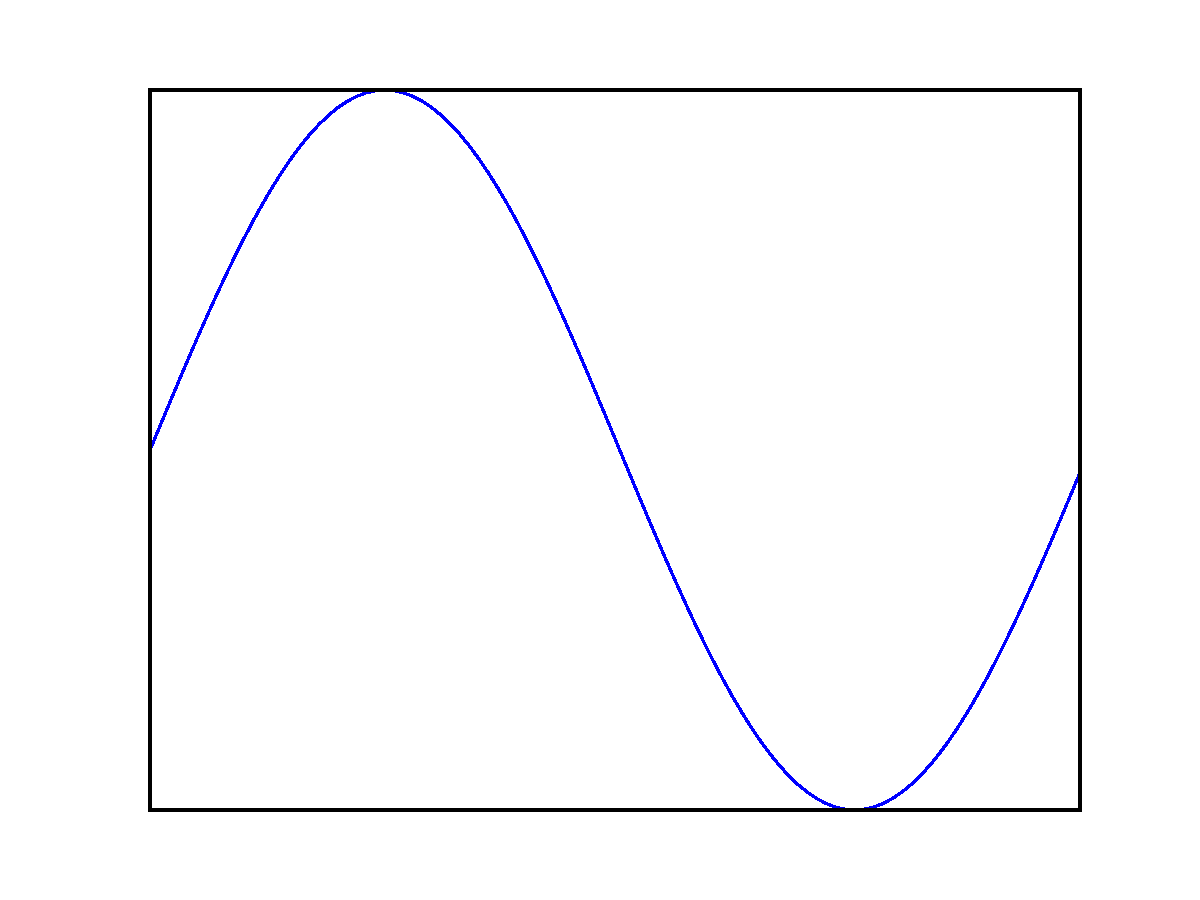
\includegraphics[scale=0.2]{figures/1d_manifold.pdf}%{figures/continuous-pyramid.pdf}
		}
		\end{subfloat}~
		\begin{subfloat}[Continuous Embedding Decomposed with Adaptive Octree]{%
			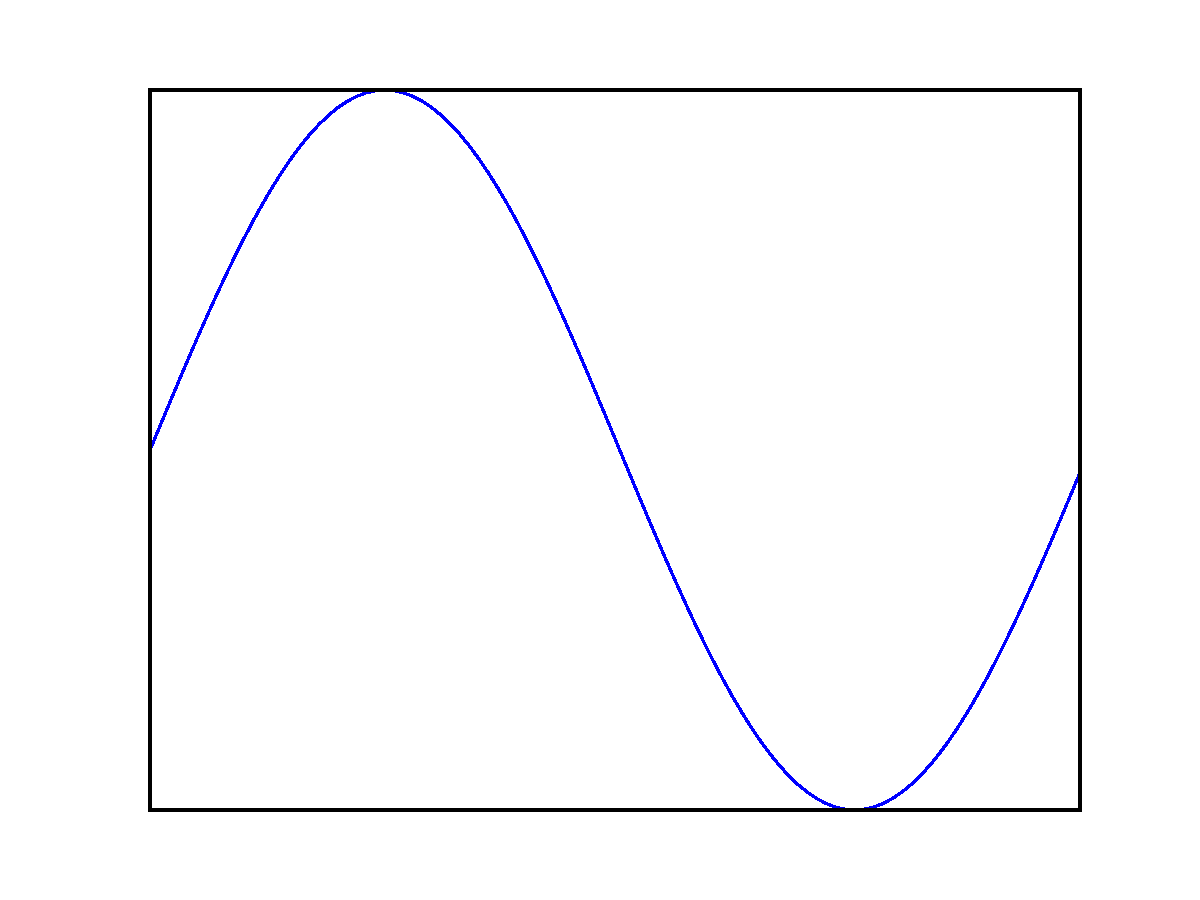
\includegraphics[scale=0.2]{figures/1d_manifold.pdf}%{figures/continuous-pyramid.pdf}
		}
		\end{subfloat}
	\end{center}

	\caption{Static and Adaptive Decomposition of Datasets}
	\label{fig:static-adaptive-decomposition}
\end{figure}

TODO: something about databases and different statistical distributions - PT WORKS WELL ON THAT FROM LIT BUT NOT THIS STUFF

Figure \ref{fig:non-continuous-embedding} shows a dataset computed using the mapping $f : \mathbb{R}^1 \rightarrow \mathbb{R}^2$. Unlike the astrophysics dataset, $f$ is not modelling continuous physical phenomenon and a such, the resulting dataset in $\mathbb{R}^2$ is not continuous (i.e. is not a curve). This would be the case for the synthetic data randomly generated for performance analysis previously. In this particular example,. 

Figure \ref{fig:continuous-embedding-pyramid} shows a continuous one-dimensional manifold. It is similar to the astrophysics dataset in that many points are aligned along some value close to the boundary. The Pyramid Tree ends up storing all the points in just threes buckets. Without the ability to adapt, the performance of the structure will rapidly degrade as more and more points are mapped to the same bucket. Figure \ref{fig:continuous-embedding-octree} shows an adaptive Octree decomposition, which adapts the decomposition by providing greater discrimination between points in regions that contain more points.

The point $kd$-tree can be seen as an adaptive index structure to some extent, since decomposition of the underlying data space depends on the values of the given points. This, along with its resilience to points aligned in strips close to boundaries, are some of the reasons its performance is vastly superior to the Pyramid Tree for the two scientific datasets.

\section{Suitability of Dimension Reduction Techniques}

The Pseudo-Pyramid Tree and Pyramid Tree both produce a static decomposition of the underlying data space through the use of dimension reduction. They do not adapt to the distribution of the input data by modifying the amount or size of bins. With dynamic data, where one does not know the distribution of the data in advance, these approaches are severely limited. This is shown by the empirical results from this project; the performance of these two structures on the real datasets is vastly inferior to the point $kd$-tree, a simple and well-established technique.

Adaptive variants of the Pyramid Tree exist, such as the Extended Pyramid-Technique \cite{pyramid-tree} and IMinMax($\theta$) \cite{iminmax}. However, the \textit{cost} of adapting such structures limits their usefulness. For example, the Extended Pyramid-Technique moves the centre of the data space to be the median point. Doing so means that the entire structure must be rebuild, because each stored point may be hashed to a different value after the data space is moved. For large $n$ this has a massive impact on performance. Suppose the structure stores a million points and then has to adapt -- a million points must be re-inserted. IMinMax($\theta$) was implemented in this project, but the performance was still poor despite it adapting to the dataset, due of the rebuilding procedure. For this reason, it has not been covered in detail in this report and the project did not explore adaptive dimension reduction techniques any further.

Despite the more adaptive point $kd$-tree performing worse on highly skewed data like the astrophysics dataset, the structure can still process the data reasonably quickly. No major optimisations were applied to the implementation and no additional exploration was performed the numerous $kd$-tree variants that have been developed.

The empirical performance timings has lead the author of this report to conclude that techniques which perform a static decomposition of the data space are \textit{not} suitable for dynamic data, unless one knows about the kinds of distributions that will be given in advance. The supplementary theoretical analysis performed in this chapter has shown that data generated by mapping continuous domains mapped to higher-dimensional ranges are especially a challenge for structures that cannot adapt, due to the highly clustered and skewed distributions of points that result from such a mapping. Since the cost of adapting dimension reduction technique is so high due to rebuilds being required, perhaps dimension reduction in general is not suitable for dynamic data.

Index structures which can adapt to different distributions of data \textit{as} points are inserted tend to require less computation and from initial experimentation with the point $kd$-tree, they appear to offer good performance. Further examples of such structures include the KDB-tree and splay quadtree (see Sections \ref{sec:recursive-partition-structures} and \ref{sec:history-sensitive-structures}).

\section{New Hypotheses}

Based on the empirical evidence from Chapter \ref{chap:design-and-implementation} and the theoretical evaluation from Chapter \ref{chap:technical-evaluation}, the hypothesis from Section \ref{sec:main-hypothesis} has been abandoned in favour of the following new hypothesis.

\paragraph{\textbf{HYPOTHESIS 1:}} Pyramid Tree is not a suitable index structure for higher-dimensional scientific datasets where there is a high amount of sparsity and large clusters of points at data space boundaries or aligned in strips along certain dimensions. TODO: mention attributes

\paragraph{\textbf{HYPOTHESIS 2:}} Dimension reduction or hash-based index structures cannot adapt well to dynamically changing distributions of data.

\paragraph{\textbf{HYPOTHESIS 3:}} Dynamic tree-based structures, which decompose the data space ,

\paragraph{}

Hypothesis 1 has been verified specifically for the astrophysics (and to a lesser extent, the hurricane Isabel dataset), but more research and analysis with other scientific datasets is required. Hypotheses 2 and 3 also require additional research to verify, but this is beyond the scope of this project. 

TODO: refer to future work section OR ACTUALLY HAVE FUTURE WORK HERE???
TODO: could have work on how to VERIFY HYPOTHESES HERE
\chapter{Project Evaluation}
\label{chap:project-evaluation}
\centerline{\rule{149mm}{.02in}}
\vspace{2cm}

This section will evaluate the project as whole, discussing its process and succes. Limitations of the project are discussed and proposals for future work in this field are also proposed.

\section{Process Evaluation}

TODO

\section{Objectives and Minimum Requirements}

Sections \ref{sec:objectives} and \ref{sec:requirements} lists the project's objectives and minimum requirements respectively. The minimum requirements were developed so that meeting them also meets the project's objectives. For brevity, the minimum requirements will be referred to by their numbers.

Requirement 1 was met by producing a literature review which has been placed in this report. The challenges of multi-dimensional search were summarised, most classes of index structures were discussed in some way and a taxonomy showing how index structures have affected each other was developed. The literature review itself was comprehensive

Requirement 2 was met by implementing the initial Pseudo-Pyramid Tree implementation, which was analysed at the end of Section \ref{sec:iteration1}. This requirement was largely exceeded, since a total of twelve implementations were developed for this project. Eight of these implementations being discussed and analysed with respect to both performance timings and their general behaviour (e.g. bucket size and balance factor). Due to time constraints, the remaining four structures could not be discussed and evaluated in detail. These are described in Appendix \ref{chap:additional-structures}.

Requirement 3 was met by optmising the Pseudo-Pyramid Tree hashing function both algorithmically and through SSE. Several implementations of the hash-based index structures were developed to reduce cache misses and computation. Several additional structures were also implemented to determine which provides the best performance for the target datasets. Therefore, this requirement was also exceeded.

Evaluation was present throughout the Chapters \ref{chap:design-and-implementation} and \ref{chap:technical-evaluation}, meaning Requirement 4 has been met. Again, the requirement was exceeded because three evaluations based on empirical performance timings were performed, along with a separate evaluation of the high-level algorithms deriving insight into what kind of index structures may be suitable for the project's target data.

Therefore, all the minimum requirements were met and exceeded to varying degrees. In particular, the amount of optimisations and index structures that were implemented and evaluation was much larger than intended. This was done to ensure the evaluation was a comprehensive as possible within the three months of the project.

\section{Deliverables}

The deliverables described in Section \ref{sec:deliverables} were all produced in the following ways:
\begin{enumerate}
	\item Source code of the evaluation framework and all implemented structures, along with documentation, accompanies this recursive-partition-structures
	\item A user manual describing the data formats and how to use select index structures is provided in Appendix \ref{chap:user-manual}
	\item An evaluation of the index structures was performed as part of Requirement 4
	\item Generated synthetic data can be re-produced using the data generators provided in the source code of deliverable 1
\end{enumerate}

\section{Limitations}

TODO

\section{Future Work}

TODO: verify hypotheses

 Structures similar to the $kd$-tree include the KDB-tree and splay quadtree (see Sections \ref{sec:recursive-partition-structures} and \ref{sec:history-sensitive-structures}).

\begin{itemize}
	\item Exploration of kd-tree variants
	\item Embedding or distance-based methods
	\item More exploration of adaptive dimension reduction techniques
	\item Parallel kd-trees, since they seem to perform well
\end{itemize}

\section{Conclusion}

TODO: general conclusion to project findings and stuff

The overall aim of the project was to implement one or more index structures and evaluate their performance with respective to high-dimensional datasets (i.e. $d > 10$). Using the astrophysics dataset as a test case, the evaluation went into much greater detail than initially expected. A greater number of index structures and optimisations were implemented than planning, resulting in a more comprehensive evaluation. Therefore, the project's aim has been met and exceeded.

Furthermore, the evaluation resulted in a conjecture and several hypotheses being made. Doing so has created a foundation for future work to be started. Considering the project has resulted in several index structures being implemented, which have been evaluated in detail, and provided a platform for future work, I would consider the project a success.

\addcontentsline{toc}{chapter}{\numberline { }Bibliography}
\bibliographystyle{unsrt}
\bibliography{refs}      % include the bibliography

\appendix                % include the appendices
\chapter{Personal Reflection}
\vspace{-0.75cm}
\centerline{\rule{149mm}{.02in}}
\vspace{0.75cm}

During my time in industry last year, I worked on several projects end-to-end. Each project provided their own unique challenges, which drove me to improve both my technical and professional skills to the level required to deliver. This project was no exception.

I will admit that, after returning to university with several projects under my belt, I was not expecting the final year project to be as difficult as I found it. I had experience with gathering requirements, deciding project scope and deliverables and communicating the motivation and progress of such projects to invested parties. What separated this project from others I have done was the heavy focus on independent research and the amount of critical thinking required to make the necessary decisions. Multi-dimensional search is a huge research area, much bigger than I had imagined. I started the project with very little knowledge on the field, so even just deciding the scope of the project required a significant amount of time and thought. Every decision required me to think carefully and objectively. Is this the right data to use? Is this the right structure to implement? Is this a fair and unbiased evaluation approach?

The project had many ups and downs. There were times everything seemed to go right and times I made the wrong decisions and was burnt by it. A lot of time at the start was spent planning all the work to be done throughout the three months of the project. Despite the time spent on the plan, many of this had to be changed or adapted on-the-fly to react to unexpected change. During the middle of the project, the core hypothesis driving my actions was disproved by the results of an evaluation. I had to react quickly and make sure I used the knowledge gained from the evaluation to steer the project in another direction, developing a new plan. I found this very challenging to do. Nevertheless, the project as a whole was a satisfying experience and I have definitely learnt from it.

\section{What I Have Learned}

I have learnt much from this project, but the especially valuable lessons were:
\begin{itemize}
	\item \textbf{Background Research} -- I have learnt how to dive into a field I have very little knowledge about, find relevant literature in a methodical way and synthesise that literature into higher-level insights about the field.
	\item \textbf{Risk Management} -- research projects generally involve high amounts of risks and I believe this project was no exception. This project's implementation phase in particular carried lots of risk -- a structure could take longer to implement than expected, may not perform as well as expected or I might even fail to find the necessary information to implement the structure (e.g. the Splay Quadtree). I had to become better at planning for risk and mitigating its effects to ensure the project continued running smoothly.
	\item \textbf{Methodical Evaluation} -- this is the first project that has required me to perform such an in-depth, rigorous evaluation. It required \textit{thinking} about what I am doing and why at all times and a systematic approach to support this thinking. The project has has improved my ability to do this, by methodically evaluating the results of experiments and deriving new insights.
	\item \textbf{Technical Skills} -- the sheer amount of algorithms reviewed, created and modified for this report has improved my algorithm design skills. Additionally, I have learnt how to write efficient code by considering cache coherency, memory management and how the underlying C/C++ code works.
\end{itemize}

\section{What I Would Do Differently}

The biggest mistake made in this project was not following a systematic and methodical approach. If a truly systematic approach was followed with the evaluation of the implementations, then the problems with the Pyramid Tree should have been caught some in the first two weeks of the Design and Implementation phase, not the fourth week like it was. The discovery was made too late in the project, making it difficult to steer the project in a different direction in time.

Further mistakes were made after this discovery. Rather than perform an in-depth evaluation into \textit{why} the Pyramid Tree had such bad performance straight away, other structures were explored. However, these were all other hash-based structures, which as shown in the final technical evaluation in this report, are likely to always perform poorly with the target datasets. I should have had the discipline to stop and think about the reason for the poor performance of the Pyramid Tree, rather than rushing into implementing other structures without considering the wider implications of the findings. By the time I had realised this, it was late into the project.

\section{Advice to Fellow Students}

The main advice I'd give to students who are yet to start their final year projects, or anyone starting any kind of project, is to \textbf{not be afraid of making the wrong decisions}. One has to have the courage to make decisions, since that's the only way to achieve the desired outcome. Nearly everything worth doing involves some measure of risk and has the possibility of failure. I would even argue that most ``right" decisions are found by making previously wrong decisions and understanding \textit{why} they were wrong. Such is the nature of the scientific method.

I started the implementation phase of my project with a hypothesis I wanted to prove. Early test results matched my hypothesis. When this happened, I could have simply stopped the evaluation there and deemed my hypothesis to be correct. However, not satisfied my evaluation was comprehensive enough, I continued to perform more and more tests and eventually found out my hypothesis turned out to be wrong. Initially, I was frustrated that I spent so much time implementing something which ended up proving the exact opposite of what I wanted to find. However, I realised that these results, even if it was not what I wanted to find, are valuable. Losing the fear of making wrong decisions/hypotheses allows one to maintain skepticism. Never try and fit the data to a hypothesis or have a biased interpretation. In fact, try as hard as possible to break hypotheses; rigorous skepticism is the only way one can be truly confident in their work and defend it against criticism from others.

Another piece of advice I have is to \textbf{always think of the bigger picture}. Always remember what the project is actually trying to achieve, \textit{why} this achievement is useful and where the current task fits into a greater context of the project and its domain. It is very easy to get caught up in small technical details about specific tools or implementations which do not move the project forward. Constantly re-evaluate where the project is, what work is currently being done and if that work is actually getting the project any closer to its goal. There were a couple of times where I spend days trying to implement certain functionality before taking a step back and re-evaluating the situation to determine if what I was implementing was truly worth the time investment. This is especially important since the project's timeframe is so short.

Finally, \textbf{be realistic about the project's goals}. Ambition causes people to force themselves into situations that will push them to learn more, which is good, but the project is short. Furthermore, large chunks of this short timeframe will be spent on background research and writing the mid-project/final reports. Therefore, students are not expected to develop the latest and greatest techniques/applications. It is getting experience in the \textit{process} which is the valuable part. The process of diving into a new field, identifying where a contribution can be made, making a commitment on what to deliver and following through with that commitment, managing the inevitable changes that will occur throughout. Embracing this process will allow the project go much smoother and induce less stress.

\section{Final Remarks}

While the end results were not as efficient as I had wanted, I hope someone will find use in the project's deliverables and findings for their own work in the future. I greatly enjoyed this project, even if I probably spent far too many evenings in the lab. I found myself becoming highly interested in multi-dimensional search and I have only scratched the surface of it. 

The project was challenging at times, but without those challenges it would not have been as satisfying to complete. While I would like to revisit the problem again someday, I believe think the project was repeatedly steered in the wrong directions due to poor decision making and lack of systematic approach. While I have learnt many lessons from this project, the result of this project leads me to believe I not cut out for research.
\chapter{Record of External Materials Used}
\centerline{\rule{149mm}{.02in}}
\vspace{2cm}

I developed all of the materials presented in this project myself.


\chapter{Ethical Issues}
\vspace{-0.75cm}
\centerline{\rule{149mm}{.02in}}
\vspace{0.75cm}

There are no ethical issues involved with this project, as no personal data is being used in either the design, implementation or evaluation of the solution. All data used for evaluation is either synthetic data generated specifically for this project or publicly available datasets.

\chapter{Supplementary Material}
\label{chap:supp-material}
\centerline{\rule{149mm}{.02in}}
\vspace{2cm}

TODO: intro to section

\begin{landscape}

	\null  % Empty line
	\nointerlineskip  % No skip for prev line
	\vfill
	\let\snewpage \newpage
	\let\newpage \relax
		\begin{figure}[H]
			\centering
			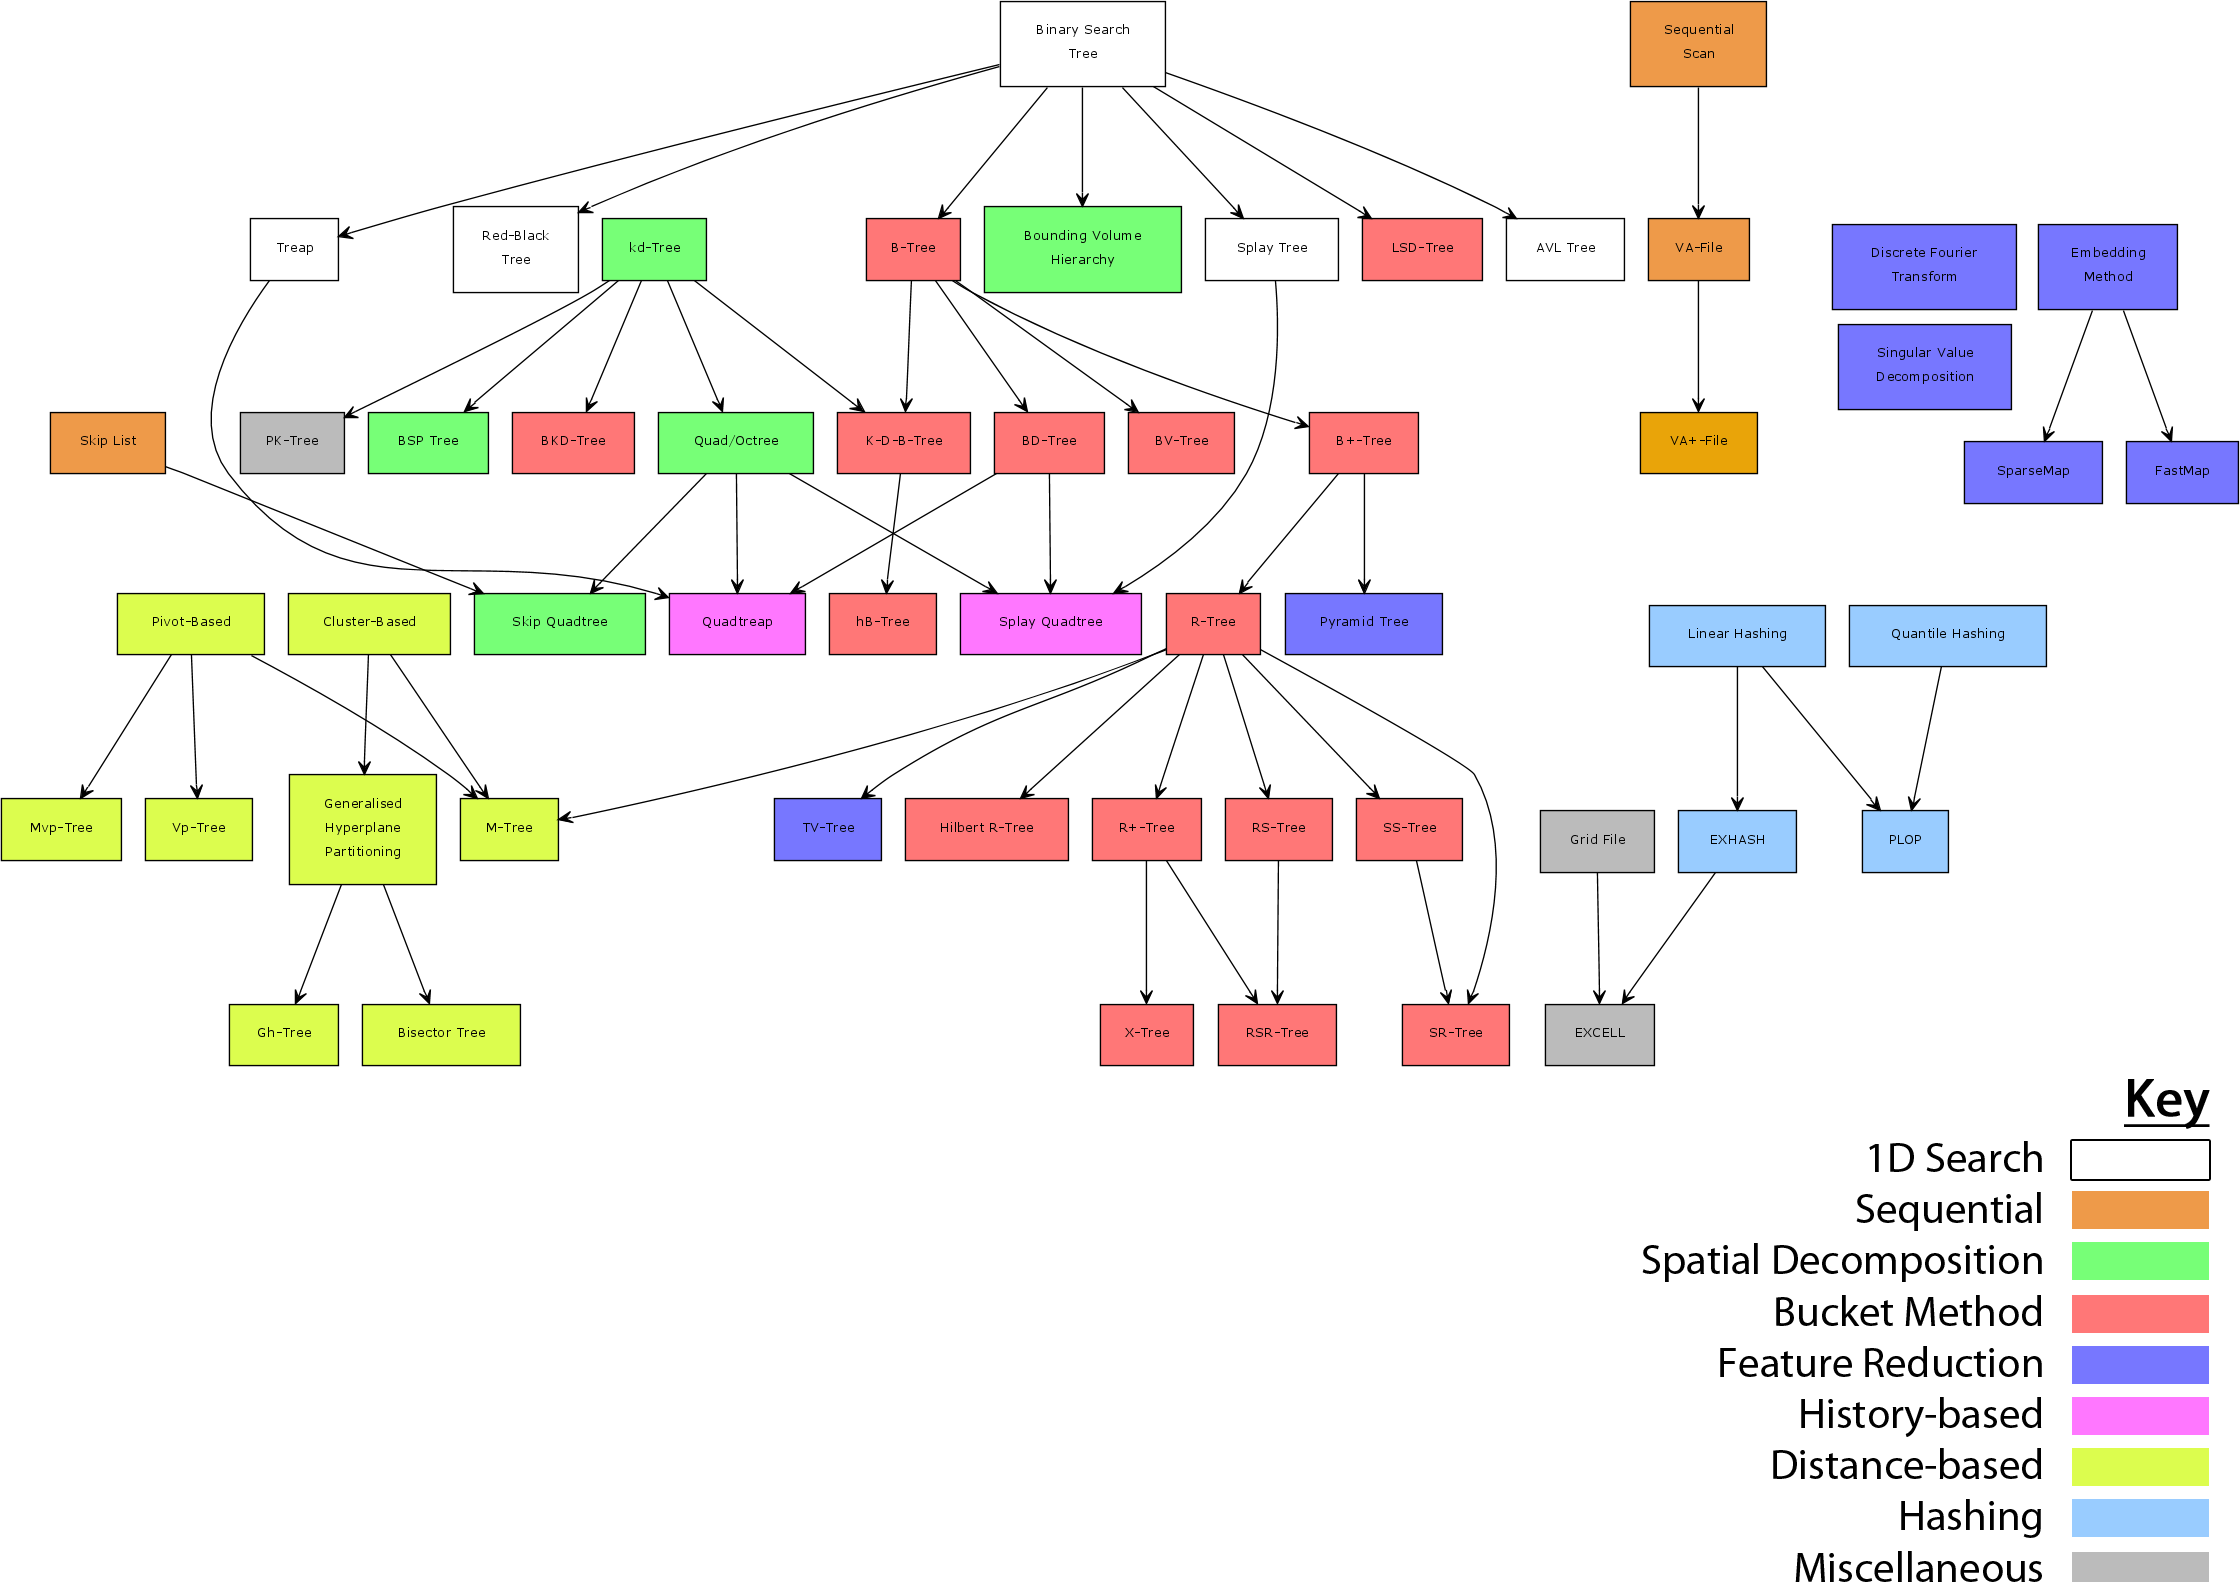
\includegraphics[scale=0.35]{figures/md_structure_taxonomy.png}
			\caption{Multi-dimensional Search Structure Taxonomy}
			\label{fig:structure-taxonomy}
		\end{figure}
	\let \newpage \snewpage
	\vfill 
	\break % page break

	\newpage

	\begin{table}
		\centering
		\begin{tabular}{|p{2.8cm}|p{5cm}|p{5cm}|p{5cm}|p{2cm}|}
			\hline
			\textbf{Index Structure} &
			\textbf{Memory Overhead} &
			\textbf{Bucket Method?} &
			\textbf{High-Dimensional Data} &
			\textbf{Complexity} \\
			\hline
			Sequential Scan & Low & No (but since data is stored contiguously, there are minimal I/O operations due to sequential access) & Often better than other structures with high $d$ (but significantly poorer performance with low $d$) & Low \\		
			B${}^{+}$-Tree & Low & Yes & One-dimensional & Low \\
			R-Tree & Moderate & Yes & Poor for $d > 10$ \cite{pyramid-tree} & Moderate \\
			Quadtree & Low with uniformly distributed data, high for skewed data due to unnecessary nodes caused by splitting sparse regions of data space & No & Poor because it tries to use balanced splits \cite{pyramid-tree} & Low \\
			Pyramid Tree & Low & Yes (based on B${}^{+}$-tree) & Good & High \\
			PK-Tree & Moderate & No (but uses similar method to reduce I/O operations) & Good & High \\
			Skip Quadtree & Moderate & No & Untested & Moderate \\
			Quadtreap & Low & No & Untested & Moderate \\
			Splay Quadtree & Moderate & No & Untested & Moderate \\
			\hline
		\end{tabular}
		\caption{Comparison of Dynamic Multi-Dimensional Structures}
		\label{tab:comparison}
	\end{table}

\end{landscape}

=ITERATION 1=
TODO: tables showing times for three operations w/ synthetic and clustered data (two tables)

TODO: plots for three operations w/ synthetic and clustered data (6 plots)

=ITERATION 2=
TODO: tables showing times for three operations w/ synthetic and clustered data (two tables)

TODO: plots not in main report (7 plots)
\chapter{Supplementary Evaluation Measures}
\label{chap:performance-timings}
\centerline{\rule{149mm}{.02in}}
\vspace{2cm}

This section contains tables and plots containing performance timings or other evaluation measures that are not vital to the overall evaluation and discussion in the main report. They are provided here for completeness.

\begin{landscape}

	\section{Iteration 1}
	\label{sec:appendix-perf1}

	Tables containing the execution times of each structure evaluated in iteration 1 for all synthetic datasets in provided in this section. When ``-" is shown instead of the number of seconds, it means that the performance test could not finish due to the machine running out of memory.

	\begin{table}[h]
		\centering
		\makebox[\textwidth][c]{%
			\begin{tabular}{|r|r|l|l|l|l|l|l|l|l|}
				\hline
				\multicolumn{2}{|c}{} & \multicolumn{8}{|c|}{\textbf{Dimensions}} \\
				\hline
				\textbf{Structure} & \textbf{Operation} & 1 & 2 & 3 & 5 & 10 & 50 & 100 & 200 \\
				\hline
	\multirow{3}{*}{Sequential Scan} & Delete & 0.470472 & 0.592127 & 0.697993 & 0.698381 & 0.628591 & 0.869429 & 1.481980 & 3.310680 \\
	& Insert & 0.084579 & 0.094937 & 0.085707 & 0.095868 & 0.111307 & 0.135492 & 0.144736 & 0.146832 \\ 
	& Point Query & 0.083401 & 0.089991 & 0.084615 & 0.094284 & 0.110552 & 0.134057 & 0.143772 & 0.143288 \\ 
	\hline
	\multirow{3}{*}{Octree} & Delete & 0.036083 & 0.002966 & 0.022031 & 0.010735 & 0.141340 & - & - & - \\
	& Insert & 0.003538 & 0.003241 & 0.003617 & 0.010450 & 0.266260 & - & - & - \\ 
	& Point Query & 0.002353 & 0.002051 & 0.002198 & 0.005085 & 0.087902 & - & - & - \\ 
	\hline
				\multirow{3}{*}{Rebuild Index PPT} & Delete & 0.018730 & 0.018783 & 0.018869 & 0.019018 & 0.019110 & 0.020654 & 0.022705 & 0.027272 \\
	& Insert & 0.002354 & 0.002281 & 0.002370 & 0.002437 & 0.002467 & 0.004444 & 0.006765 & 0.012032 \\ 
	& Point Query & 0.000356 & 0.000412 & 0.000470 & 0.000579 & 0.000741 & 0.002066 & 0.003858 & 0.007477 \\ 
	\hline
	\multirow{3}{*}{Bucket PPT} & Delete & 0.030306 & 0.001195 & 0.001240 & 0.001285 & 0.001448 & 0.002732 & 0.004719 & 0.008228 \\
	& Insert & 0.003278 & 0.003304 & 0.003396 & 0.003432 & 0.003546 & 0.004528 & 0.005974 & 0.008790 \\ 
	& Point Query & 0.000587 & 0.000637 & 0.000691 & 0.000767 & 0.000958 & 0.002089 & 0.003791 & 0.007132 \\ 
	\hline
	\multirow{3}{*}{Splay PPT} & Delete & 0.001615 & 0.001697 & 0.001796 & 0.001832 & 0.002074 & 0.003294 & 0.005372 & 0.009422 \\
	& Insert & 0.005308 & 0.005349 & 0.005434 & 0.005503 & 0.005368 & 0.006438 & 0.007978 & 0.010943 \\ 
	& Point Query & 0.001167 & 0.001215 & 0.001272 & 0.001320 & 0.001542 & 0.002722 & 0.004591 & 0.008136 \\ 
	\hline
			\end{tabular}
		}%

		\caption{Total Execution Time (in seconds) of Each Operation for Varying Number of Dimensions for Points in Uniform Distribution}
		\label{tab:perf1-dimensionality-uniform}
	\end{table}

	\begin{table}[h]
		\centering
		\makebox[\textwidth][c]{%
			\begin{tabular}{|r|r|l|l|l|l|l|l|l|l|}
				\hline
				\multicolumn{2}{|c}{} & \multicolumn{8}{|c|}{\textbf{Dimensions}} \\
				\hline
				\textbf{Structure} & \textbf{Operation} & 1 & 2 & 3 & 5 & 10 & 50 & 100 & 200 \\
				\hline
\multirow{3}{*}{Sequential Scan} & Delete & 0.472209 & 0.587695 & 0.698374 & 0.698280 & 0.628742 & 0.870596 & 1.470970 & 3.189490 \\
	& Insert & 0.084389 & 0.095311 & 0.091186 & 0.096900 & 0.111276 & 0.135272 & 0.142041 & 0.138340 \\ 
	& Point Query & 0.084033 & 0.090757 & 0.089855 & 0.095227 & 0.110525 & 0.134670 & 0.139539 & 0.131027 \\ 
	\hline
				\multirow{3}{*}{Rebuild Index PPT} & Delete & 0.018436 & 0.018667 & 0.018746 & 0.018938 & 0.019339 & 0.020980 & 0.023090 & 0.027601 \\
	& Insert & 0.002063 & 0.002185 & 0.002297 & 0.002191 & 0.002425 & 0.004455 & 0.006863 & 0.012370 \\ 
	& Point Query & 0.000401 & 0.000483 & 0.000601 & 0.000785 & 0.001088 & 0.002385 & 0.004057 & 0.007745 \\ 
	\hline
	\multirow{3}{*}{Octree} & Delete & 0.003181 & 0.002863 & 0.002899 & 0.004750 & 0.060280 & - & - & - \\
	& Insert & 0.003490 & 0.003123 & 0.003417 & 0.006512 & 0.096882 & - & - & - \\ 
	& Point Query & 0.002517 & 0.002092 & 0.002068 & 0.003469 & 0.038702 & - & - & - \\ 
	\hline
	\multirow{3}{*}{Bucket PPT} & Delete & 0.001151 & 0.001285 & 0.001400 & 0.001586 & 0.001798 & 0.003149 & 0.005718 & 0.010378 \\
	& Insert & 0.003048 & 0.003033 & 0.003047 & 0.002641 & 0.002733 & 0.004051 & 0.005955 & 0.009829 \\ 
	& Point Query & 0.000622 & 0.000711 & 0.000799 & 0.000980 & 0.001235 & 0.002473 & 0.004487 & 0.008423 \\ 
	\hline
	\multirow{3}{*}{Splay PPT} & Delete & 0.001666 & 0.001799 & 0.001966 & 0.002073 & 0.002207 & 0.003627 & 0.006075 & 0.010744 \\
	& Insert & 0.004809 & 0.004528 & 0.004295 & 0.003763 & 0.003639 & 0.005462 & 0.007504 & 0.011415 \\ 
	& Point Query & 0.001191 & 0.001263 & 0.001373 & 0.001454 & 0.001655 & 0.003052 & 0.005191 & 0.009122 \\ 
	\hline
			\end{tabular}
		}%

		\caption{Total Execution Time (in seconds) of Each Operation for Varying Number of Dimensions for Points in Skewed Distribution}
		\label{tab:perf1-dimensionality-skewed}
	\end{table}

	\begin{table}[h]
		\centering
		\makebox[\textwidth][c]{%
			\begin{tabular}{|r|r|l|l|l|l|l|l|l|l|}
				\hline
				\multicolumn{2}{|c}{} & \multicolumn{8}{|c|}{\textbf{Dimensions}} \\
				\hline
				\textbf{Structure} & \textbf{Operation} & 1 & 2 & 3 & 5 & 10 & 50 & 100 & 200 \\
				\hline
	\multirow{3}{*}{Sequential Scan} & Delete & 0.452688 & 0.587081 & 0.697896 & 0.698466 & 0.628546 & 0.891051 & 1.462300 & 3.001740 \\
	& Insert & 0.083242 & 0.094424 & 0.085648 & 0.096576 & 0.111202 & 0.132845 & 0.128193 & 0.152179 \\ 
	& Point Query & 0.082480 & 0.089000 & 0.084912 & 0.095301 & 0.110343 & 0.131766 & 0.127011 & 0.139105 \\ 
	\hline
				\multirow{3}{*}{Rebuild Index PPT} & Delete & 0.017734 & 0.018559 & 0.018705 & 0.031202 & 0.031609 & 0.036050 & 0.038830 & 0.043520 \\
	& Insert & 0.002046 & 0.002063 & 0.002034 & 0.013408 & 0.013477 & 0.015667 & 0.018618 & 0.024482 \\ 
	& Point Query & 0.000377 & 0.000478 & 0.000624 & 0.012120 & 0.012301 & 0.013848 & 0.015801 & 0.019471 \\ 
	\hline
	\multirow{3}{*}{Octree} & Delete & 0.002921 & 0.002943 & 0.003555 & 0.008215 & 0.196480 & - & - & - \\
	& Insert & 0.003374 & 0.003168 & 0.004207 & 0.008885 & 0.200285 & - & - & - \\ 
	& Point Query & 0.002290 & 0.002197 & 0.002620 & 0.006860 & 0.174983 & - & - & - \\ 
	\hline
	\multirow{3}{*}{Bucket PPT} & Delete & 0.001081 & 0.001228 & 0.001326 & 0.004807 & 0.005011 & 0.006451 & 0.008927 & 0.013484 \\
	& Insert & 0.003032 & 0.002788 & 0.002410 & 0.009184 & 0.009169 & 0.010462 & 0.012720 & 0.017194 \\ 
	& Point Query & 0.000578 & 0.000697 & 0.000762 & 0.007699 & 0.007923 & 0.009395 & 0.011409 & 0.015258 \\ 
	\hline
	\multirow{3}{*}{Splay PPT} & Delete & 0.001477 & 0.001544 & 0.001488 & 0.004813 & 0.005030 & 0.006421 & 0.008874 & 0.013484 \\
	& Insert & 0.004490 & 0.003715 & 0.003146 & 0.009693 & 0.009611 & 0.010749 & 0.013051 & 0.017751 \\ 
	& Point Query & 0.001035 & 0.001037 & 0.000952 & 0.007720 & 0.007979 & 0.009394 & 0.011464 & 0.015449 \\ 
	\hline
			\end{tabular}
		}%

		\caption{Total Execution Time (in seconds) of Each Operation for Varying Number of Dimensions for Points in Clustered Distribution}
		\label{tab:perf1-dimensionality-clustered}
	\end{table}
	
\begin{table}[h]
	\centering
	\makebox[\textwidth][c]{%
		\begin{tabular}{|r|r|l|l|l|}
			\hline
			\multicolumn{2}{|c}{} & \multicolumn{3}{|c|}{\textbf{Number of Points}} \\
			\hline
			\textbf{Structure} & \textbf{Operation} & 10000 & 100000 & 500000 \\
			\hline
\multirow{3}{*}{Sequential Scan} & Delete & 0.684460 & 69.043000 & 1767.620000 \\
& Insert & 0.124515 & 15.434500 & 603.073000 \\ 
& Point Query & 0.123733 & 14.959700 & 596.142000 \\ 
\hline
			\multirow{3}{*}{Rebuild Index PPT} & Delete & 0.019048 & 1.992800 & 50.793300 \\
& Insert & 0.002543 & 0.039762 & 0.214066 \\ 
& Point Query & 0.000808 & 0.015071 & 0.099620 \\ 
\hline
\multirow{3}{*}{Bucket PPT} & Delete & 0.001528 & 0.025504 & 0.168358 \\
& Insert & 0.003496 & 0.057898 & 0.322042 \\ 
& Point Query & 0.000988 & 0.015642 & 0.105091 \\ 
\hline
\multirow{3}{*}{Splay PPT} & Delete & 0.002118 & 0.039638 & 0.343901 \\
& Insert & 0.005708 & 0.087068 & 0.592703 \\ 
& Point Query & 0.001626 & 0.034237 & 0.315927 \\ 
\hline
		\end{tabular}
	}%

	\caption{Total Execution Time (in seconds) of Each Operation for Varying Number of Points in Uniformly Distributed Synthetic Dataset}
	\label{tab:perf1-size}
\end{table}

\end{landscape}

\begin{landscape}

	\section{Iteration 3}
	\label{sec:appendix-perf3}

	Tables containing the execution times of each structure evaluated in iteration 3 for all synthetic datasets in provided in this section.

	\begin{table}[h]
		\centering
		\makebox[\textwidth][c]{%
			\begin{tabular}{|r|r|l|l|l|l|l|l|l|l|}
				\hline
				\multicolumn{2}{|c}{} & \multicolumn{8}{|c|}{\textbf{Dimensions}} \\
				\hline
				\textbf{Structure} & \textbf{Operation} & 1 & 2 & 3 & 5 & 10 & 50 & 100 & 200 \\
				\hline
				\multirow{3}{*}{Bucket Hash Table} & Delete & 0.000962 & 0.001165 & 0.001359 & 0.001767 & 0.002753 & 0.010661 & 0.020123 & 0.039643 \\
	& Insert & 0.003657 & 0.003903 & 0.004099 & 0.004499 & 0.005349 & 0.013639 & 0.022934 & 0.042463 \\ 
	& Point Query & 0.000521 & 0.000813 & 0.000992 & 0.001394 & 0.002390 & 0.010282 & 0.019494 & 0.038578 \\ 
	\hline
	\multirow{3}{*}{$kd$-tree} & Delete & 0.002989 & 0.003472 & 0.003969 & 0.004823 & 0.005603 & 0.006942 & 0.007316 & 0.009964 \\
	& Insert & 0.002171 & 0.002204 & 0.002277 & 0.002390 & 0.002412 & 0.002957 & 0.003238 & 0.004987 \\ 
	& Point Query & 0.002018 & 0.002033 & 0.002113 & 0.002286 & 0.002388 & 0.003076 & 0.003868 & 0.006119 \\ 
	\hline
	\multirow{3}{*}{Bucket PPT} & Delete & 0.060140 & 0.001183 & 0.016044 & 0.004926 & 0.002860 & 0.003024 & 0.004981 & 0.008579 \\
	& Insert & 0.003387 & 0.003402 & 0.003371 & 0.003488 & 0.003901 & 0.005354 & 0.006898 & 0.009913 \\ 
	& Point Query & 0.000596 & 0.000650 & 0.000683 & 0.000741 & 0.000890 & 0.002223 & 0.003984 & 0.007371 \\ 
	\hline
	\multirow{3}{*}{Pyramid Tree} & Delete & 0.001028 & 0.001179 & 0.001287 & 0.001430 & 0.001613 & 0.003569 & 0.005926 & 0.010783 \\
	& Insert & 0.003283 & 0.003442 & 0.003448 & 0.003630 & 0.003856 & 0.005487 & 0.007401 & 0.011192 \\ 
	& Point Query & 0.000557 & 0.000663 & 0.000715 & 0.000881 & 0.001122 & 0.002896 & 0.005028 & 0.009483 \\ 
	\hline
			\end{tabular}
		}%

		\caption{Total Execution Time (in seconds) of Each Operation for Varying Number of Dimensions for Points in Uniform Distribution}
		\label{tab:perf3-dimensionality-uniform}
	\end{table}

	\begin{table}[h]
		\centering
		\makebox[\textwidth][c]{%
			\begin{tabular}{|r|r|l|l|l|l|l|l|l|l|}
				\hline
				\multicolumn{2}{|c}{} & \multicolumn{8}{|c|}{\textbf{Dimensions}} \\
				\hline
				\textbf{Structure} & \textbf{Operation} & 1 & 2 & 3 & 5 & 10 & 50 & 100 & 200 \\
				\hline
				\multirow{3}{*}{Bucket Hash Table} & Delete & 0.000950 & 0.001153 & 0.001398 & 0.001754 & 0.002715 & 0.010399 & 0.020252 & 0.040310 \\
	& Insert & 0.003520 & 0.003885 & 0.004107 & 0.004437 & 0.005318 & 0.013232 & 0.022708 & 0.042113 \\ 
	& Point Query & 0.000510 & 0.000789 & 0.001000 & 0.001382 & 0.002382 & 0.010002 & 0.019695 & 0.039192 \\ 
	\hline
	\multirow{3}{*}{$kd$-tree} & Delete & 0.002911 & 0.003400 & 0.003990 & 0.004584 & 0.005309 & 0.006993 & 0.007280 & 0.009264 \\
	& Insert & 0.002158 & 0.002190 & 0.002325 & 0.002356 & 0.002362 & 0.002729 & 0.003344 & 0.005076 \\ 
	& Point Query & 0.002072 & 0.002085 & 0.002198 & 0.002250 & 0.002320 & 0.002940 & 0.004033 & 0.006363 \\ 
	\hline
	\multirow{3}{*}{Bucket PPT} & Delete & 0.001129 & 0.001311 & 0.001404 & 0.001567 & 0.001715 & 0.003100 & 0.005837 & 0.011133 \\
	& Insert & 0.003103 & 0.003043 & 0.003121 & 0.002771 & 0.002762 & 0.004453 & 0.006723 & 0.010688 \\ 
	& Point Query & 0.000625 & 0.000750 & 0.000814 & 0.000982 & 0.001199 & 0.002469 & 0.004794 & 0.009071 \\ 
	\hline
	\multirow{3}{*}{Pyramid Tree} & Delete & 0.001038 & 0.001174 & 0.001341 & 0.001462 & 0.001752 & 0.003932 & 0.006805 & 0.012752 \\
	& Insert & 0.003096 & 0.003368 & 0.003466 & 0.003604 & 0.003888 & 0.005053 & 0.007492 & 0.012443 \\ 
	& Point Query & 0.000555 & 0.000635 & 0.000752 & 0.000890 & 0.001249 & 0.003232 & 0.005814 & 0.010997 \\ 
	\hline
			\end{tabular}
		}%

		\caption{Total Execution Time (in seconds) of Each Operation for Varying Number of Dimensions for Points in Skewed Distribution}
		\label{tab:perf3-dimensionality-skewed}
	\end{table}

	\begin{table}[h]
		\centering
		\makebox[\textwidth][c]{%
			\begin{tabular}{|r|r|l|l|l|l|l|l|l|l|}
				\hline
				\multicolumn{2}{|c}{} & \multicolumn{8}{|c|}{\textbf{Dimensions}} \\
				\hline
				\textbf{Structure} & \textbf{Operation} & 1 & 2 & 3 & 5 & 10 & 50 & 100 & 200 \\
				\hline
				\multirow{3}{*}{Bucket Hash Table} & Delete & 0.000927 & 0.001112 & 0.001354 & 0.001651 & 0.002513 & 0.009530 & 0.018395 & 0.036484 \\
	& Insert & 0.003368 & 0.003819 & 0.004049 & 0.004349 & 0.005112 & 0.012236 & 0.020933 & 0.038674 \\ 
	& Point Query & 0.000493 & 0.000753 & 0.000946 & 0.001285 & 0.002204 & 0.009126 & 0.017825 & 0.035381 \\ 
	\hline
	\multirow{3}{*}{$kd$-tree} & Delete & 0.003257 & 0.003522 & 0.003926 & 0.005384 & 0.007460 & 0.009404 & 0.011730 & 0.014420 \\
	& Insert & 0.002268 & 0.002168 & 0.002241 & 0.002390 & 0.002412 & 0.002506 & 0.003285 & 0.004643 \\ 
	& Point Query & 0.002142 & 0.002025 & 0.002081 & 0.002296 & 0.002349 & 0.002713 & 0.003940 & 0.005929 \\ 
	\hline
	\multirow{3}{*}{Bucket PPT} & Delete & 0.001069 & 0.001261 & 0.001352 & 0.004816 & 0.005001 & 0.006457 & 0.009281 & 0.013836 \\
	& Insert & 0.003049 & 0.002917 & 0.002505 & 0.009361 & 0.009485 & 0.010845 & 0.013384 & 0.017897 \\ 
	& Point Query & 0.000575 & 0.000690 & 0.000791 & 0.007716 & 0.007960 & 0.009414 & 0.011603 & 0.015418 \\ 
	\hline
	\multirow{3}{*}{Pyramid Tree} & Delete & 0.001016 & 0.001179 & 0.001375 & 0.001435 & 0.001683 & 0.003667 & 0.006479 & 0.011976 \\
	& Insert & 0.003041 & 0.003345 & 0.003504 & 0.003575 & 0.003980 & 0.005496 & 0.007778 & 0.012194 \\ 
	& Point Query & 0.000542 & 0.000637 & 0.000758 & 0.000871 & 0.001212 & 0.002997 & 0.005691 & 0.010567 \\ 
	\hline
			\end{tabular}
		}%

		\caption{Total Execution Time (in seconds) of Each Operation for Varying Number of Dimensions for Points in Clustered Distribution}
		\label{tab:perf3-dimensionality-clustered}
	\end{table}

	\begin{table}[h]
		\centering
		\makebox[\textwidth][c]{%
			\begin{tabular}{|r|r|l|l|l|l|}
				\hline
				\multicolumn{2}{|c}{} & \multicolumn{4}{|c|}{\textbf{Number of Points}} \\
				\hline
				\textbf{Structure} & \textbf{Operation} & 10000 & 100000 & 500000 & 1000000 \\
				\hline
				\multirow{3}{*}{Bucket Hash Table} & Delete & 0.003926 & 0.050295 & 0.277580 & 0.578340 \\
	& Insert & 0.006568 & 0.081556 & 0.463257 & 0.962260 \\ 
	& Point Query & 0.003515 & 0.043550 & 0.249102 & 0.516167 \\ 
	\hline
	\multirow{3}{*}{$kd$-tree} & Delete & 0.005552 & 0.144179 & 1.264420 & 2.967910 \\
	& Insert & 0.002401 & 0.062702 & 0.565952 & 1.367600 \\ 
	& Point Query & 0.002408 & 0.061273 & 0.537383 & 1.330470 \\ 
	\hline
	\multirow{3}{*}{Bucket PPT} & Delete & 0.001580 & 0.025124 & 0.164381 & 0.350934 \\
	& Insert & 0.003628 & 0.060662 & 0.326802 & 0.675884 \\ 
	& Point Query & 0.001059 & 0.016118 & 0.105968 & 0.245357 \\ 
	\hline
	\multirow{3}{*}{Pyramid Tree} & Delete & 0.002060 & 0.031297 & 0.211423 & 0.556193 \\
	& Insert & 0.004100 & 0.054527 & 0.379671 & 0.712960 \\ 
	& Point Query & 0.001554 & 0.025796 & 0.177153 & 0.446886 \\ 
	\hline
			\end{tabular}
		}%

		\caption{Total Execution Time (in seconds) of Each Operation for Varying Number of Points in Uniformly Distributed Synthetic Dataset}
		\label{tab:perf3-size}
	\end{table}

\end{landscape}
\chapter{Algorithms and Code Listings}
\label{chap:algs-and-code}
\vspace{-0.75cm}
\centerline{\rule{149mm}{.02in}}
\vspace{0.75cm}

This section contains high-level pseudo-code and low-level code listings of algorithms/techniques whose details were not deemed important enough to be in the main report.

\section{Algorithms}

\begin{algorithm}[H]
	\SetAlgoLined
	\SetKwInOut{Input}{input}\SetKwInOut{Output}{output}
	\SetKwFunction{hashPoint}{hashPoint} \SetKwFunction{hashFloat}{hashFloat}

 	\SetKwProg{funcHashPoint}{Algorithm}{}{}
  	\funcHashPoint{\hashPoint{$d, p$}} {
		\Input{$d$ = number of dimensions}
		\Input{$p_0, p_1, \dots, p_{d-1}$ = coordinates of point}
		\Output{$seed$ = integer representing hashed point}
		\Begin {
			$seed = 0$\;
			\For{$i = 0$ to $d - 1$} {
				$seed = seed \oplus \left(\hashFloat(p_i) + \texttt{0x9e3779b9} + (seed << 6) + (seed >> 2)\right)$
			}
			\KwRet{$seed$}
		}
	}

	\caption{Hashing Multi-Dimensional Point in Bucket Hash Table}
	\label{alg:point-hashing}
\end{algorithm}

\paragraph{\textbf{NOTE:}} \texttt{hashFloat} is a function which hashes an individual 32-bit floating point number and corresponds to the function \texttt{float\_hash\_impl2} in Listing \ref{lst:hash-float-function}.

\newpage

\section{Code Listings}

\begin{lstlisting}[label=lst:hash-float-function, caption=Code to Hash Single 32-bit Floating Point Value (Source code from file \texttt{boost/functional/hash/detail/hash\_float\_generic.hpp} in Boost Library 1.42.0)]
// Copyright 2005-2009 Daniel James.
// Distributed under the Boost Software License, Version 1.0. (See accompanying
// file LICENSE_1_0.txt or copy at http://www.boost.org/LICENSE_1_0.txt)

// A general purpose hash function for non-zero floating point values.

inline void hash_float_combine(std::size_t& seed, std::size_t value)
{
    seed ^= value + (seed<<6) + (seed>>2);
}

template <class T>
inline std::size_t float_hash_impl2(T v)
{
    boost::hash_detail::call_frexp<T> frexp;
    boost::hash_detail::call_ldexp<T> ldexp;

    int exp = 0;

    v = frexp(v, &exp);

    // A postive value is easier to hash, so combine the
    // sign with the exponent and use the absolute value.
    if(v < 0) {
        v = -v;
        exp += limits<T>::max_exponent -
            limits<T>::min_exponent;
    }

    // The result of frexp is always between 0.5 and 1, so its
    // top bit will always be 1. Subtract by 0.5 to remove that.
    v -= T(0.5);
    v = ldexp(v, limits<std::size_t>::digits + 1);
    std::size_t seed = static_cast<std::size_t>(v);
    v -= seed;

    // ceiling(digits(T) * log2(radix(T))/ digits(size_t)) - 1;
    std::size_t const length
        = (limits<T>::digits *
                boost::static_log2<limits<T>::radix>::value - 1)
        / limits<std::size_t>::digits;

    for(std::size_t i = 0; i != length; ++i)
    {
        v = ldexp(v, limits<std::size_t>::digits);
        std::size_t part = static_cast<std::size_t>(v);
        v -= part;
        hash_float_combine(seed, part);
    }

    hash_float_combine(seed, exp);

    return seed;
}
\end{lstlisting}
\chapter{Additional Index Structures}
\label{chap:additional-structures}
\vspace{-0.75cm}
\centerline{\rule{149mm}{.02in}}
\vspace{0.75cm}

This section describes index structures which were implemented during the project, but were not discussed or evaluated in the main report due to time constraints. Preliminary findings on the structures' performance is discussed.

\section{Multigrid}
\label{sec:multigrid}

The Multigrid decomposes the data space into a uniform grid by cutting each dimension into $B$ intervals. A cell is defined by the intervals of each dimension it is contained in. Formally, a cell $C = \lbrace c_0, c_1, \dots, c_{d - 1} \rbrace$, where $c_i$ is the interval the cell belongs to in dimension $i$. There are a total of $B^d$ cells. Figure \ref{fig:multigrid-decomposition} illustrates how the Multigrid decomposes 2D data space when $B = 5$. Each cell corresponds to a bucket in the Multigrid structure.

This structure is a hybrid of hash-based and tree-based structures. It is a tree where each leaf node is a bucket containing one or more points and non-leaves are hash tables. Each non-leaf hashes points to the interval in a specific dimension $i$ the point is contained in. The bucket a point is hashed to is another node of the Multigrid tree. This node is either another hash table, which hashes points based on which interval of dimension $i + 1$ they are inside, or a simple bucket.

The root node always hashes points to which interval of dimension 0 they are contained in. When these buckets exceed a certain capacity, say $M$, then the bucket is turned into a hash table which hash points to their interval in dimension 1. This is repeated until the last dimension, $d - 1$, is reached. At this point, there are no more dimensions to discriminate points with, so the buckets are not transformed into hash tables when their size exceeds $M$. 

In effect, this creates a tree where the maximum height is $d + 1$ and each non-leaf node has at most $B$ children that correspond to the $B$ intervals of the dimension it is discriminating against. All non-leaf nodes at level $i$ of the tree hash points to the interval of dimension $i$ they are stored in. The hashing function for dimension $i$ is given below:

\begin{equation}
	h_i(p) = \floor*{\frac{p_i - min_i}{max_i - min_i} \times B}
	\label{eq:multigrid-hash}
\end{equation}
where $p$ is a point and $min_i, max_i$ are the lower and upper boundaries of dimension $i$.

Figure \ref{fig:multigrid-root} shows a Multigrid tree with a single non-leaf node and its accompanying spatial decomposition in 2D. Notice how points are discriminated only using the value of the $x$ dimension. Figure \ref{fig:multigrid-multiple-levels} shows a Multigrid where some of the bucket sizes have exceeded $M$, which is 3 in this case. Notice how some intervals in the $x$ dimension have been sliced in the $y$ dimension now, allowing for greater discrimination.

Equation \ref{eq:multigrid-hash} can clearly be computed in constant time. Since there are at most $d + 1$ levels in the tree, at most $d$ instances of Equation \ref{eq:multigrid-hash} will be computed. It follows that retrieving the bucket a point is contained in takes $O(d)$ time. If points are uniformly distributed across the data space, then this structure will take $O(d)$ time for all operations.  However, it is possible for all the points in a dataset to be mapped to the same cell, making \texttt{insert}, \texttt{delete} and point query operations take O$(n)$ time.

For highly skewed datasets, most of the points will end up being mapped to the same few cells. This causes the structure to degenerate to Sequential Scan in a similar manner to the Pyramid Tree (see Section \ref{sec:implications-to-md-search}). Figure \ref{fig:multigrid-clustered} illustrates the core limitation. Despite both dimensions being used to discriminate between points, they are all get hashed to the same value as they are contained in the same cell.

\begin{figure}
	\begin{center}
		\begin{subfloat}[Multigrid Tree Decomposition\label{fig:multigrid-decomposition}]{%
			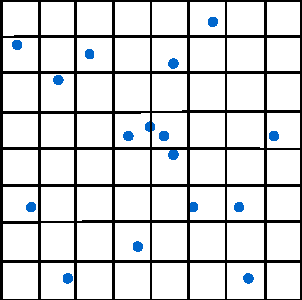
\includegraphics[scale=0.65]{figures/multigrid_decomposition.pdf}
		}
		\end{subfloat}~~~~~
		\begin{subfloat}[t][Multigrid Tree with Clustered Data\label{fig:multigrid-clustered}]{%
			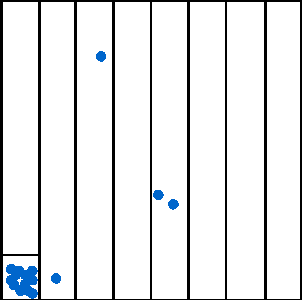
\includegraphics[scale=0.65]{figures/multigrid_clustered.pdf}
		}
		\end{subfloat}
	\end{center}

	\caption{Multigrid Decompositions}
	\label{fig:multigrid-decompositions}
\end{figure}

\begin{figure}
	\begin{center}
		\begin{subfloat}[Multigrid Tree with Minimum Height\label{fig:multigrid-root}]{%
			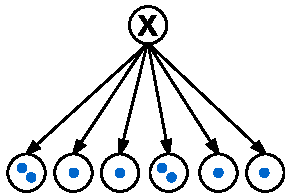
\includegraphics[scale=0.65]{figures/multigrid_root_tree.pdf}
			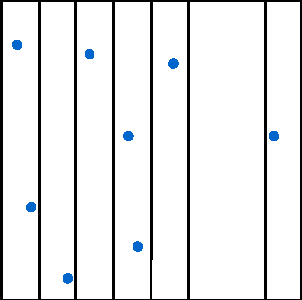
\includegraphics[scale=0.65]{figures/multigrid_root.pdf}
		}
		\end{subfloat}~~~~~
		\begin{subfloat}[Multigrid Tree with Maximum Height\label{fig:multigrid-multiple-levels}]{%
			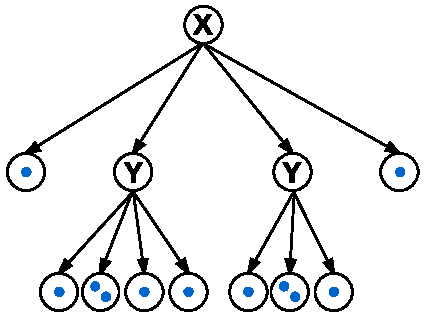
\includegraphics[scale=0.65]{figures/multigrid_levels_tree.pdf}
			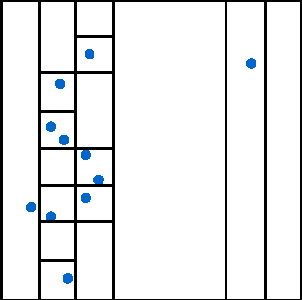
\includegraphics[scale=0.65]{figures/multigrid_levels.pdf}
		}
		\end{subfloat}
	\end{center}

	\caption{Multigrid Trees and their Respective Spatial Decompositions in 2D}
	\label{fig:multigrid-trees}
\end{figure}

\section{iMinMax($\theta$)}

iMinMax($\theta$) is an index structure similar to the Pyramid Tree, whose behaviour is affected by the parameter $\theta$ \cite{iminmax}. $\theta$ can be tuned to optimise the structure for different data distributions. Like the Pyramid Tree, it reduces points to a single dimension and applies a one-dimensional index structure to these values. To adapt to a dynamic distribution, the value of $\theta$ is tweaked, changing the hashing function. This means the structure must be rebuild every time $\theta$ is changed.

An implementation of this was developed by modifying the existing Bucket Pseudo-Pyramid Tree implementation (see Section \ref{sec:iteration1}). Preliminary tests revealed that the structure was only slightly faster than the Pyramid Tree for the astrophysics and hurricane Isabel datasets, regardless of which value was chosen for $\theta$. The majority of the structure's execution time was spent rebuilding the structure, supporting the claim that existing dimension reduction techniques will require rebuilding are not suitable for dynamic data (discussed in Section \ref{sec:implications-to-md-search}).

\section{Bucket $kd$-Tree}

Instead of storing a single point in every node of the tree, the \textbf{Bucket $kd$-Tree} stores multiple points in each node (termed a bucket), with the constraint that only leaf nodes store points. Non-leaf nodes serve to partition the data space, each cutting the space along a single dimension by some value (the cutting value). When the number of points in a leaf exceeds a certain number, say $M$, then a cutting dimension and value are determined, which is used to split a leaf into two. The left and right children nodes are leaves that contain the points from the split node that lie on one of the sides of the split.

To query or delete a point, the leaf containing the point is found, which is sequentially scanned to find the point. If the point is found, it is removed from the leaf. If the total number of points being stored in the modified leaf node and its sibling is less than $\frac{M}{4}$, then the two leaf nodes are \textit{merged} into their parent. The parent becomes a leaf node containing all the points stored in the two leaves.

Compared to the point $kd$-tree, the bucket $kd$-tree has more knowledge about the distribution of the points since multiple are stored in a bucket. With the point $kd$-tree, only one point at a time is used to determine the cutting dimension, so less knowledge about the distribution is used to perform a split. Knowing more about the distribution allows the bucket $kd$-tree to partition the data more effectively to construct a more balanced tree.

This structure was implemented as part of the project. The \textit{sliding midpoint} splitting rule was used to split full leaves, which is described in \cite{sliding-midpoint-split}. Preliminary results show that it reduced balance factor, but an inefficient implementation meant there were large constant factors that dominated performance. This made the structure slower than the point $kd$-tree implementation. More work optimising the implementation should be performed to assess its suitability for dynamic scientific datasets.
\chapter{mdsearch Documentation}
\label{chap:mdsearch}
\vspace{-0.75cm}
\centerline{\rule{149mm}{.02in}}
\vspace{0.75cm}

mdsearch is a small C++ library that implements a subset of the index structures discussed in this report. The library is available to download on an online Git repository \footnote{\url{https://github.com/DonaldWhyte/mdsearch}}. This library makes heavy use of template metaprogramming and inline functions to boost performance. As such, it is a header-only library. Each implemented index structure can be used by simply including its corresponding header file.

TODO: change bucket hash table to bit hash

Currently, the following index structures have been implemented:
\begin{itemize}
	\item \textbf{Pyramid Tree} -- see Section \ref{sec:pyramid-tree-detail} for more information
	\item \textbf{$kd$-Tree} -- see Section \ref{sec:kd-tree-detail} for more information
	\item \textbf{Bucket Hash Table} -- see Section \ref{sec:bit-hash} for more information
	\item \textbf{Multigrid} -- see Section \ref{sec:multigrid} for more information
\end{itemize}

\section{Dependencies}

mdsearch requires the following header-only Boost libraries
\begin{itemize}
	\item Boost.Unordered
	\item Boost.Functional/Hash
	\item Boost.Lexical\_Cast
\end{itemize}

\section{API}

Each index structure is represented as a class, which implements the three operations evaluated in the project. Therefore, each index structure class has the following methods:
\begin{itemize}
	\item \texttt{bool insert(point)} -- inserts unique point into the structure. Returns true if point insertion was successful and false if point is already being stored and has not been inserted.
	\item \texttt{bool remove(point)} -- deletes point from structure. Returns true if the point was found and deleted successful and false if the point was not found.
	\item \texttt{bool query(point)} -- returns true if point is being stored in structure and false otherwise.
\end{itemize}

Table \ref{tab:library-classes} describes the role of each class in the library. Figure \ref{fig:library-class-diagram} illustrates the inheritance and dependencies between these classes using a UML class diagram.

\begin{table}[H]
	\centering
	\begin{tabular}{|p{4.25cm}|p{9.5cm}|}
		\hline
		\textbf{Data Type} & \textbf{Description} \\
		\hline
		\texttt{Real} & Type of individual coordinate of point \\
		\texttt{RealList} & Re-sizeable array of \texttt{Real}s \\
		\texttt{HashType} & Type of discrete hash value used by hash-based structures \\
		\texttt{Point<D>} & Point with D dimensions \\
		\texttt{Boundary<D>} & Boundary in D-dimensional space \\
		\texttt{Dataset<D>} & Dataset containing D-dimension points, which can load points from files and compute the minimum bounding region containing every point \\
		\texttt{KDTree<D>} & $kd$-tree for D-dimensional space \\
		\texttt{Multigrid<D>} & Multigrid for D-dimensional space \\
		\texttt{HashStructure<D>} & Abstract class for hash-based structures, which follows the Bucket Pseudo-Pyramid Tree structure described in Section \ref{sec:iteration1} closely \\
		\texttt{PyramidTree<D>} & Pyramid Tree for D-dimensional space \\
		\texttt{BucketHashTable<D>} & Bucket Hash Table for D-dimensional space \\
		\hline
	\end{tabular}
	\caption{Descriptions of Each Type in mdsearch Library}
	\label{tab:library-classes}
\end{table}

\begin{figure}[H]
	\centering
	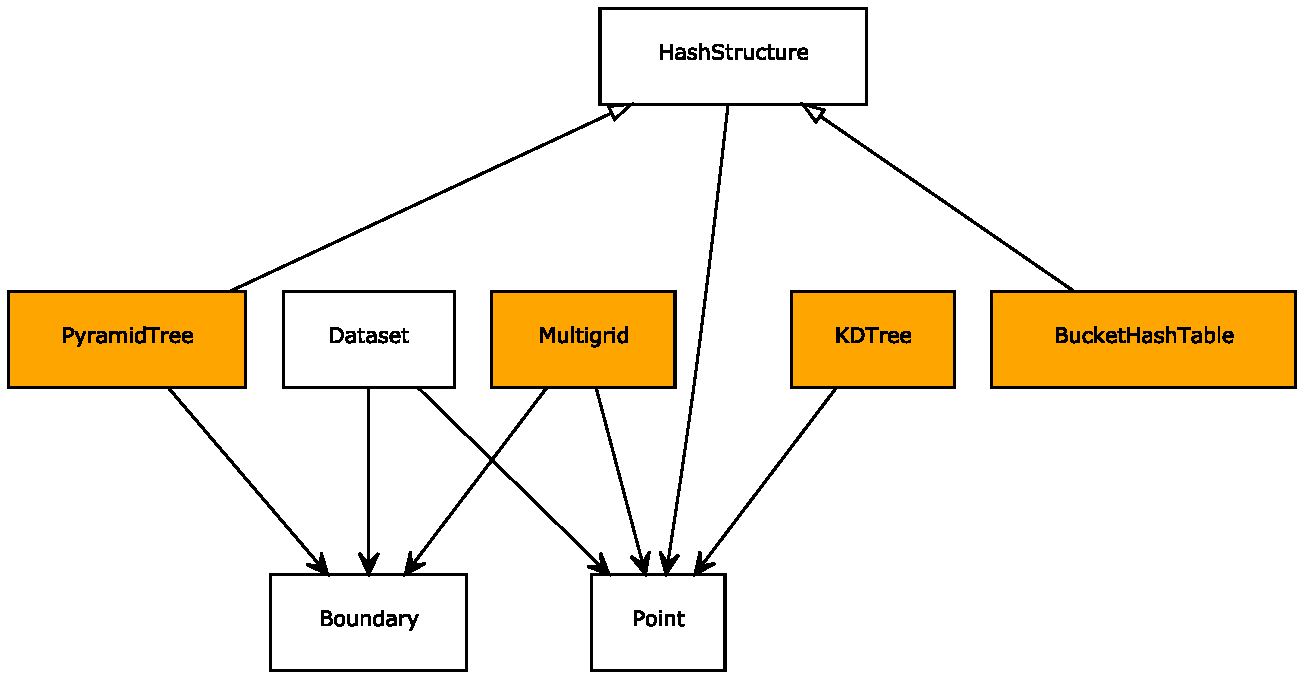
\includegraphics[scale=0.6]{figures/mdsearch_classes_uml.pdf}
	\caption{UML Class Diagram of mdsearch Library. Coloured Boxes Represent Index Structures.}
	\label{fig:library-class-diagram} 
\end{figure}

\section{Examples}

The library comes with a program that generates random points and performs a set of correctness tests on each index structure. This program is contained within the \texttt{test\_structures.cpp} file and as such ,

\end{document}
